%% set-up
\documentclass[a4paper,12pt,twoside,openany]{book}

%% define metadata
\def \booktitle {Viking Tales}
\def \authorname {Jennie Hall}
\def \illustrator {Victor R. Lambdin}
\def \keywords {folklore}
\def \licenseurl {
    https://www.gutenberg.org/wiki/Gutenberg:Permission_How-To}
\def \producers {
    Bryan Ness, Stephen Blundell and the Online Distributed Proofreading
    Team at \url{http://www.pgdp.net} (This file was produced from images
    generously made available by The Internet Archive/American
    Libraries.)}
\def \ebooknumber {24811}
\def \releasedate {March 12, 2008}

%% title page, info
\def \thetitlepage {
    
\includegraphics[width=8.1cm]{viking-tales/003}

    \vfill

    Copyright, 1902,\\
    By \scshape{Jennie Hall}

    
\includegraphics[width=2.7cm]{viking-tales/004}

    Made in U.S.A.
    \newpage

    \begin{figure}
        \centering
        
\includegraphics[width=4cm]{viking-tales/001}
        \\[5cm]
        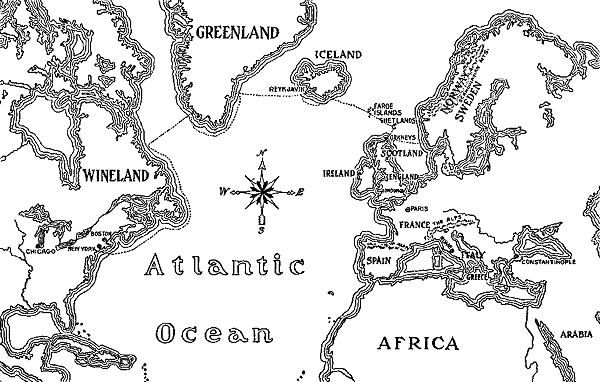
\includegraphics[width=\textwidth]{viking-tales/002}
        \caption{A map showing the journeys of the Vikings}
    \end{figure}
}
\def \bookinfo {
    Title: \booktitle \\
    Author: \authorname \\
    Illustrator: \illustrator \\
    Release Date: \releasedate \\
    eBook number: \ebooknumber \\
    Produced by \producers
}
\def \preface {}

%% style file containing template
\usepackage{../../template}

%% additional configurations
% remove chapter numbering
\renewcommand{\thechapter}{}
% remove "chapter"
\renewcommand{\chaptername}{\vspace{-30pt}}
% remove title of lof and adjust spacing
\renewcommand*\listfigurename{\vspace{-70pt}}
% remove figure numbering
\renewcommand{\thefigure}{}
% no caption label; italic and large font
\captionsetup{labelformat=empty,font={it,large}}
%%% sectsty options
\chapterfont{\mdseries\Huge\centering\scshape\lowercase}
\sectionfont{\mdseries\scshape\LARGE\centering\lowercase}
\partfont{\mdseries\Huge\itshape}
\parttitlefont{\mdseries\Huge\scshape\lowercase}
%%% tocloft options
% toc chapter number width
\setlength{\cftchapnumwidth}{0em}
% lof chapter number width
\setlength{\cftfignumwidth}{0em}
% lof font style
\renewcommand{\cftfigfont}{\itshape}
% part display in toc
\renewcommand{\cftpartfont}{\Large\scshape\hfill}

%% lettrine fonts
\input Carrickc.fd
\newcommand*\initfamily{\usefont{U}{Carrickc}{xl}{n}}
% set lettrine to use initial font and specified color
\renewcommand\LettrineFontHook{\initfamily}

%% new part figure
\def \partfig {
    \newpage
    \begin{figure}
        \noindent\rule{\textwidth}{.4pt}
        \vskip8pt
        \centering
        
\includegraphics[width=4cm]{viking-tales/001}
        \noindent\rule{\textwidth}{.4pt}
    \end{figure}
}

\def \thetableofcontents {
    \chapter*{
\includegraphics[width=9.3cm]{viking-tales/005}}
    % remove toc name and adjust spacing
    \renewcommand\contentsname{\vspace{-70pt}}
    \tableofcontents
    \chapter[A List of the Illustrations]{
        
\includegraphics[width=9.3cm]{viking-tales/006}}
    \listoffigures
}
%%%
\begin{document}

    \thefrontmatter
    \chapter*{Ivanhoe\\
    A Romance}

\begin{verse}
Now fitted the halter, now traversed the cart,\\
And often took leave,--but seemed loath to depart!\footnote{The motto
alludes to the Author returning to the stage
repeatedly after having taken leave.}\\!
\attrib{--Prior.}
\end{verse}

\chapter{Introduction to Ivanhoe}

\lettrine{T}{he Author} of the Waverley Novels had hitherto proceeded in
an unabated
course of popularity, and might, in his peculiar district of literature,
have been termed ``L'Enfant Gate'' of success. It was plain, however,
that frequent publication must finally wear out the public favour,
unless some mode could be devised to give an appearance of novelty to
subsequent productions. Scottish manners, Scottish dialect, and Scottish
characters of note, being those with which the author was most
intimately, and familiarly acquainted, were the groundwork upon which he
had hitherto relied for giving effect to his narrative. It was, however,
obvious, that this kind of interest must in the end occasion a degree of
sameness and repetition, if exclusively resorted to, and that the reader
was likely at length to adopt the language of Edwin, in Parnell's Tale:

``\,`Reverse the spell,' he cries, `And let it fairly now suffice. The
gambol has been shown.'\,''

Nothing can be more dangerous for the fame of a professor of the fine
arts, than to permit (if he can possibly prevent it) the character of a
mannerist to be attached to him, or that he should be supposed capable
of success only in a particular and limited style. The public are, in
general, very ready to adopt the opinion, that he who has pleased them
in one peculiar mode of composition, is, by means of that very talent,
rendered incapable of venturing upon other subjects. The effect of this
disinclination, on the part of the public, towards the artificers of
their pleasures, when they attempt to enlarge their means of amusing,
may be seen in the censures usually passed by vulgar criticism upon
actors or artists who venture to change the character of their efforts,
that, in so doing, they may enlarge the scale of their art.

There is some justice in this opinion, as there always is in such as
attain general currency. It may often happen on the stage, that an
actor, by possessing in a preeminent degree the external qualities
necessary to give effect to comedy, may be deprived of the right to
aspire to tragic excellence; and in painting or literary composition, an
artist or poet may be master exclusively of modes of thought, and powers
of expression, which confine him to a single course of subjects. But
much more frequently the same capacity which carries a man to popularity
in one department will obtain for him success in another, and that must
be more particularly the case in literary composition, than either in
acting or painting, because the adventurer in that department is not
impeded in his exertions by any peculiarity of features, or conformation
of person, proper for particular parts, or, by any peculiar mechanical
habits of using the pencil, limited to a particular class of subjects.

Whether this reasoning be correct or otherwise, the present author felt,
that, in confining himself to subjects purely Scottish, he was not only
likely to weary out the indulgence of his readers, but also greatly to
limit his own power of affording them pleasure. In a highly polished
country, where so much genius is monthly employed in catering for public
amusement, a fresh topic, such as he had himself had the happiness to
light upon, is the untasted spring of the desert;--

``Men bless their stars and call it luxury.''

But when men and horses, cattle, camels, and dromedaries, have poached
the spring into mud, it becomes loathsome to those who at first drank of
it with rapture; and he who had the merit of discovering it, if he would
preserve his reputation with the tribe, must display his talent by a
fresh discovery of untasted fountains.

If the author, who finds himself limited to a particular class of
subjects, endeavours to sustain his reputation by striving to add a
novelty of attraction to themes of the same character which have been
formerly successful under his management, there are manifest reasons
why, after a certain point, he is likely to fail. If the mine be not
wrought out, the strength and capacity of the miner become necessarily
exhausted. If he closely imitates the narratives which he has before
rendered successful, he is doomed to ``wonder that they please no
more.'' If he struggles to take a different view of the same class of
subjects, he speedily discovers that what is obvious, graceful, and
natural, has been exhausted; and, in order to obtain the indispensable
charm of novelty, he is forced upon caricature, and, to avoid being
trite, must become extravagant.

It is not, perhaps, necessary to enumerate so many reasons why the
author of the Scottish Novels, as they were then exclusively termed,
should be desirous to make an experiment on a subject purely English. It
was his purpose, at the same time, to have rendered the experiment as
complete as possible, by bringing the intended work before the public as
the effort of a new candidate for their favour, in order that no degree
of prejudice, whether favourable or the reverse, might attach to it, as
a new production of the Author of Waverley; but this intention was
afterwards departed from, for reasons to be hereafter mentioned.

The period of the narrative adopted was the reign of Richard I., not
only as abounding with characters whose very names were sure to attract
general attention, but as affording a striking contrast betwixt the
Saxons, by whom the soil was cultivated, and the Normans, who still
reigned in it as conquerors, reluctant to mix with the vanquished, or
acknowledge themselves of the same stock. The idea of this contrast was
taken from the ingenious and unfortunate Logan's tragedy of Runnamede,
in which, about the same period of history, the author had seen the
Saxon and Norman barons opposed to each other on different sides of the
stage. He does not recollect that there was any attempt to contrast the
two races in their habits and sentiments; and indeed it was obvious,
that history was violated by introducing the Saxons still existing as a
high-minded and martial race of nobles.

They did, however, survive as a people, and some of the ancient Saxon
families possessed wealth and power, although they were exceptions to
the humble condition of the race in general. It seemed to the author,
that the existence of the two races in the same country, the vanquished
distinguished by their plain, homely, blunt manners, and the free spirit
infused by their ancient institutions and laws; the victors, by the high
spirit of military fame, personal adventure, and whatever could
distinguish them as the Flower of Chivalry, might, intermixed with other
characters belonging to the same time and country, interest the reader
by the contrast, if the author should not fail on his part.

Scotland, however, had been of late used so exclusively as the scene of
what is called Historical Romance, that the preliminary letter of Mr
Laurence Templeton became in some measure necessary. To this, as to an
Introduction, the reader is referred, as expressing author's purpose and
opinions in undertaking this species of composition, under the necessary
reservation, that he is far from thinking he has attained the point at
which he aimed.

It is scarcely necessary to add, that there was no idea or wish to pass
off the supposed Mr Templeton as a real person. But a kind of
continuation of the Tales of my Landlord had been recently attempted by
a stranger, and it was supposed this Dedicatory Epistle might pass for
some imitation of the same kind, and thus putting enquirers upon a false
scent, induce them to believe they had before them the work of some new
candidate for their favour.

After a considerable part of the work had been finished and printed, the
Publishers, who pretended to discern in it a germ of popularity,
remonstrated strenuously against its appearing as an absolutely
anonymous production, and contended that it should have the advantage of
being announced as by the Author of Waverley. The author did not make
any obstinate opposition, for he began to be of opinion with Dr Wheeler,
in Miss Edgeworth's excellent tale of ``Maneuvering,'' that ``Trick upon
Trick'' might be too much for the patience of an indulgent public, and
might be reasonably considered as trifling with their favour.

The book, therefore, appeared as an avowed continuation of the Waverley
Novels; and it would be ungrateful not to acknowledge, that it met with
the same favourable reception as its predecessors.

Such annotations as may be useful to assist the reader in comprehending
the characters of the Jew, the Templar, the Captain of the mercenaries,
or Free Companions, as they were called, and others proper to the
period, are added, but with a sparing hand, since sufficient information
on these subjects is to be found in general history.

An incident in the tale, which had the good fortune to find favour in
the eyes of many readers, is more directly borrowed from the stores of
old romance. I mean the meeting of the King with Friar Tuck at the cell
of that buxom hermit. The general tone of the story belongs to all ranks
and all countries, which emulate each other in describing the rambles of
a disguised sovereign, who, going in search of information or amusement,
into the lower ranks of life, meets with adventures diverting to the
reader or hearer, from the contrast betwixt the monarch's outward
appearance, and his real character. The Eastern tale-teller has for his
theme the disguised expeditions of Haroun Alraschid with his faithful
attendants, Mesrour and Giafar, through the midnight streets of Bagdad;
and Scottish tradition dwells upon the similar exploits of James V.,
distinguished during such excursions by the travelling name of the
Goodman of Ballengeigh, as the Commander of the Faithful, when he
desired to be incognito, was known by that of Il Bondocani. The French
minstrels are not silent on so popular a theme. There must have been a
Norman original of the Scottish metrical romance of Rauf Colziar, in
which Charlemagne is introduced as the unknown guest of a
charcoal-man.\footnote{This very curious poem, long a desideratum
in Scottish
literature, and given up as irrecoverably lost, was lately brought to
light by the researches of Dr Irvine of the Advocates' Library, and has
been reprinted by Mr David Laing, Edinburgh.}

It seems to have been the original of other poems of the kind.

In merry England there is no end of popular ballads on this theme. The
poem of John the Reeve, or Steward, mentioned by Bishop Percy, in the
Reliques of English Poetry,\footnote{Vol. ii. p.~167.} is said to have
turned on such an
incident; and we have besides, the King and the Tanner of Tamworth, the
King and the Miller of Mansfield, and others on the same topic. But the
peculiar tale of this nature to which the author of Ivanhoe has to
acknowledge an obligation, is more ancient by two centuries than any of
these last mentioned.

It was first communicated to the public in that curious record of
ancient literature, which has been accumulated by the combined exertions
of Sir Egerton Brydges. and Mr Hazlewood, in the periodical work
entitled the British Bibliographer. From thence it has been transferred
by the Reverend Charles Henry Hartsborne, M.A., editor of a very curious
volume, entitled ``Ancient Metrical Tales, printed chiefly from original
sources, 1829.'' Mr Hartshorne gives no other authority for the present
fragment, except the article in the Bibliographer, where it is entitled
the Kyng and the Hermite. A short abstract of its contents will show its
similarity to the meeting of King Richard and Friar Tuck.

King Edward (we are not told which among the monarchs of that name, but,
from his temper and habits, we may suppose Edward IV.) sets forth with
his court to a gallant hunting-match in Sherwood Forest, in which, as is
not unusual for princes in romance, he falls in with a deer of
extraordinary size and swiftness, and pursues it closely, till he has
outstripped his whole retinue, tired out hounds and horse, and finds
himself alone under the gloom of an extensive forest, upon which night
is descending. Under the apprehensions natural to a situation so
uncomfortable, the king recollects that he has heard how poor men, when
apprehensive of a bad nights lodging, pray to Saint Julian, who, in the
Romish calendar, stands Quarter-Master-General to all forlorn travellers
that render him due homage. Edward puts up his orisons accordingly, and
by the guidance, doubtless, of the good Saint, reaches a small path,
conducting him to a chapel in the forest, having a hermit's cell in its
close vicinity. The King hears the reverend man, with a companion of his
solitude, telling his beads within, and meekly requests of him quarters
for the night. ``I have no accommodation for such a lord as ye be,''
said the Hermit. ``I live here in the wilderness upon roots and rinds,
and may not receive into my dwelling even the poorest wretch that lives,
unless it were to save his life.'' The King enquires the way to the next
town, and, understanding it is by a road which he cannot find without
difficulty, even if he had daylight to befriend him, he declares, that
with or without the Hermit's consent, he is determined to be his guest
that night. He is admitted accordingly, not without a hint from the
Recluse, that were he himself out of his priestly weeds, he would care
little for his threats of using violence, and that he gives way to him
not out of intimidation, but simply to avoid scandal.

The King is admitted into the cell--two bundles of straw are shaken down
for his accommodation, and he comforts himself that he is now under
shelter, and that

\begin{verse}
``A night will soon be gone.''\\!
\end{verse}

Other wants, however, arise. The guest becomes clamorous for supper,
observing,

\begin{verse}
``For certainly, as I you say,\\
I ne had never so sorry a day,\\
That I ne had a merry night.''\\!
\end{verse}

But this indication of his taste for good cheer, joined to the
annunciation of his being a follower of the Court, who had lost himself
at the great hunting-match, cannot induce the niggard Hermit to produce
better fare than bread and cheese, for which his guest showed little
appetite; and ``thin drink,'' which was even less acceptable. At length
the King presses his host on a point to which he had more than once
alluded, without obtaining a satisfactory reply:

\begin{verse}
``Then said the King, 'by God's grace,\\
Thou wert in a merry place,\\
To shoot should thou here\\
When the foresters go to rest,\\
Sometyme thou might have of the best,\\
All of the wild deer;\\
I wold hold it for no scathe,\\
Though thou hadst bow and arrows baith,\\
Althoff thou best a Frere.'\,''\\!
\end{verse}

The Hermit, in return, expresses his apprehension that his guest means
to drag him into some confession of offence against the forest laws,
which, being betrayed to the King, might cost him his life. Edward
answers by fresh assurances of secrecy, and again urges on him the
necessity of procuring some venison. The Hermit replies, by once more
insisting on the duties incumbent upon him as a churchman, and continues
to affirm himself free from all such breaches of order:

\begin{verse}
``Many day I have here been,\\
And flesh-meat I eat never,\\
But milk of the kye;\\
Warm thee well, and go to sleep,\\
And I will lap thee with my cope,\\
Softly to lye.''\\!
\end{verse}

It would seem that the manuscript is here imperfect, for we do not find
the reasons which finally induce the curtal Friar to amend the King's
cheer. But acknowledging his guest to be such a ``good fellow'' as has
seldom graced his board, the holy man at length produces the best his
cell affords. Two candles are placed on a table, white bread and baked
pasties are displayed by the light, besides choice of venison, both salt
and fresh, from which they select collops. ``I might have eaten my bread
dry,'' said the King, ``had I not pressed thee on the score of archery,
but now have I dined like a prince--if we had but drink enow.''

This too is afforded by the hospitable anchorite, who dispatches an
assistant to fetch a pot of four gallons from a secret corner near his
bed, and the whole three set in to serious drinking. This amusement is
superintended by the Friar, according to the recurrence of certain
fustian words, to be repeated by every compotator in turn before he
drank--a species of High Jinks, as it were, by which they regulated
their potations, as toasts were given in latter times. The one toper
says ``fusty bandias'', to which the other is obliged to reply, ``strike
pantnere'', and the Friar passes many jests on the King's want of
memory, who sometimes forgets the words of action. The night is spent in
this jolly pastime. Before his departure in the morning, the King
invites his reverend host to Court, promises, at least, to requite his
hospitality, and expresses himself much pleased with his entertainment.
The jolly Hermit at length agrees to venture thither, and to enquire for
Jack Fletcher, which is the name assumed by the King. After the Hermit
has shown Edward some feats of archery, the joyous pair separate. The
King rides home, and rejoins his retinue. As the romance is imperfect,
we are not acquainted how the discovery takes place; but it is probably
much in the same manner as in other narratives turning on the same
subject, where the host, apprehensive of death for having trespassed on
the respect due to his Sovereign, while incognito, is agreeably
surprised by receiving honours and reward.

In Mr Hartshorne's collection, there is a romance on the same
foundation, called King Edward and the Shepherd,\footnote{Like the Hermit,
the Shepherd makes havock amongst the
King's game; but by means of a sling, not of a bow; like the Hermit,
too, he has his peculiar phrases of compotation, the sign and
countersign being Passelodion and Berafriend. One can scarce conceive
what humour our ancestors found in this species of gibberish; but ``I
warrant it proved an excuse for the glass.''}
which, considered as illustrating manners, is still more curious than
the King and the Hermit; but it is foreign to the present purpose. The
reader has here the original legend from which the incident in the
romance is derived; and the identifying the irregular Eremite with the
Friar Tuck of Robin Hood's story, was an obvious expedient.

The name of Ivanhoe was suggested by an old rhyme. All novelists have
had occasion at some time or other to wish with Falstaff, that they knew
where a commodity of good names was to be had. On such an occasion the
author chanced to call to memory a rhyme recording three names of the
manors forfeited by the ancestor of the celebrated Hampden, for striking
the Black Prince a blow with his racket, when they quarrelled at tennis:

\begin{verse}
``Tring, Wing, and Ivanhoe,\\
For striking of a blow,\\
Hampden did forego,\\
And glad he could escape so.''\\!
\end{verse}

The word suited the author's purpose in two material respects,--for,
first, it had an ancient English sound; and secondly, it conveyed no
indication whatever of the nature of the story. He presumes to hold this
last quality to be of no small importance. What is called a taking
title, serves the direct interest of the bookseller or publisher, who by
this means sometimes sells an edition while it is yet passing the press.
But if the author permits an over degree of attention to be drawn to his
work ere it has appeared, he places himself in the embarrassing
condition of having excited a degree of expectation which, if he proves
unable to satisfy, is an error fatal to his literary reputation.
Besides, when we meet such a title as the Gunpowder Plot, or any other
connected with general history, each reader, before he has seen the
book, has formed to himself some particular idea of the sort of manner
in which the story is to be conducted, and the nature of the amusement
which he is to derive from it. In this he is probably disappointed, and
in that case may be naturally disposed to visit upon the author or the
work, the unpleasant feelings thus excited. In such a case the literary
adventurer is censured, not for having missed the mark at which he
himself aimed, but for not having shot off his shaft in a direction he
never thought of.

On the footing of unreserved communication which the Author has
established with the reader, he may here add the trifling circumstance,
that a roll of Norman warriors, occurring in the Auchinleck Manuscript,
gave him the formidable name of Front-de-Boeuf.

Ivanhoe was highly successful upon its appearance, and may be said to
have procured for its author the freedom of the Rules, since he has ever
since been permitted to exercise his powers of fictitious composition in
England, as well as Scotland.

The character of the fair Jewess found so much favour in the eyes of
some fair readers, that the writer was censured, because, when arranging
the fates of the characters of the drama, he had not assigned the hand
of Wilfred to Rebecca, rather than the less interesting Rowena. But, not
to mention that the prejudices of the age rendered such an union almost
impossible, the author may, in passing, observe, that he thinks a
character of a highly virtuous and lofty stamp, is degraded rather than
exalted by an attempt to reward virtue with temporal prosperity. Such is
not the recompense which Providence has deemed worthy of suffering
merit, and it is a dangerous and fatal doctrine to teach young persons,
the most common readers of romance, that rectitude of conduct and of
principle are either naturally allied with, or adequately rewarded by,
the gratification of our passions, or attainment of our wishes. In a
word, if a virtuous and self-denied character is dismissed with temporal
wealth, greatness, rank, or the indulgence of such a rashly formed or
ill assorted passion as that of Rebecca for Ivanhoe, the reader will be
apt to say, verily Virtue has had its reward. But a glance on the great
picture of life will show, that the duties of self-denial, and the
sacrifice of passion to principle, are seldom thus remunerated; and that
the internal consciousness of their high-minded discharge of duty,
produces on their own reflections a more adequate recompense, in the
form of that peace which the world cannot give or take away.

\noindent Abbotsford, 1st September, 1830.

\chapter{Dedicatory Epistle}

\MakeLowercase{\textsc{TO}}

\noindent\MakeLowercase{\textsc{THE REV. DR DRYASDUST, F.A.S.}}

\noindent\MakeLowercase{\textsc{Residing in the Castle-Gate, York.}}

\lettrine{M}{uch} esteemed and dear Sir,
\vskip2\baselineskip

It is scarcely necessary to mention the various and concurring reasons
which induce me to place your name at the head of the following work.
Yet the chief of these reasons may perhaps be refuted by the
imperfections of the performance. Could I have hoped to render it worthy
of your patronage, the public would at once have seen the propriety of
inscribing a work designed to illustrate the domestic antiquities of
England, and particularly of our Saxon forefathers, to the learned
author of the Essays upon the Horn of King Ulphus, and on the Lands
bestowed by him upon the patrimony of St Peter. I am conscious, however,
that the slight, unsatisfactory, and trivial manner, in which the result
of my antiquarian researches has been recorded in the following pages,
takes the work from under that class which bears the proud motto,
``Detur digniori''. On the contrary, I fear I shall incur the censure of
presumption in placing the venerable name of Dr Jonas Dryasdust at the
head of a publication, which the more grave antiquary will perhaps class
with the idle novels and romances of the day. I am anxious to vindicate
myself from such a charge; for although I might trust to your friendship
for an apology in your eyes, yet I would not willingly stand conviction
in those of the public of so grave a crime, as my fears lead me to
anticipate my being charged with.

I must therefore remind you, that when we first talked over together
that class of productions, in one of which the private and family
affairs of your learned northern friend, Mr Oldbuck of Monkbarns, were
so unjustifiably exposed to the public, some discussion occurred between
us concerning the cause of the popularity these works have attained in
this idle age, which, whatever other merit they possess, must be
admitted to be hastily written, and in violation of every rule assigned
to the epopeia. It seemed then to be your opinion, that the charm lay
entirely in the art with which the unknown author had availed himself,
like a second M'Pherson, of the antiquarian stores which lay scattered
around him, supplying his own indolence or poverty of invention, by the
incidents which had actually taken place in his country at no distant
period, by introducing real characters, and scarcely suppressing real
names. It was not above sixty or seventy years, you observed, since the
whole north of Scotland was under a state of government nearly as simple
and as patriarchal as those of our good allies the Mohawks and Iroquois.
Admitting that the author cannot himself be supposed to have witnessed
those times, he must have lived, you observed, among persons who had
acted and suffered in them; and even within these thirty years, such an
infinite change has taken place in the manners of Scotland, that men
look back upon the habits of society proper to their immediate
ancestors, as we do on those of the reign of Queen Anne, or even the
period of the Revolution. Having thus materials of every kind lying
strewed around him, there was little, you observed, to embarrass the
author, but the difficulty of choice. It was no wonder, therefore, that,
having begun to work a mine so plentiful, he should have derived from
his works fully more credit and profit than the facility of his labours
merited.

Admitting (as I could not deny) the general truth of these conclusions,
I cannot but think it strange that no attempt has been made to excite an
interest for the traditions and manners of Old England, similiar to that
which has been obtained in behalf of those of our poorer and less
celebrated neighbours. The Kendal green, though its date is more
ancient, ought surely to be as dear to our feelings, as the variegated
tartans of the north. The name of Robin Hood, if duly conjured with,
should raise a spirit as soon as that of Rob Roy; and the patriots of
England deserve no less their renown in our modern circles, than the
Bruces and Wallaces of Caledonia. If the scenery of the south be less
romantic and sublime than that of the northern mountains, it must be
allowed to possess in the same proportion superior softness and beauty;
and upon the whole, we feel ourselves entitled to exclaim with the
patriotic Syrian--``Are not Pharphar and Abana, rivers of Damascus,
better than all the rivers of Israel?''

Your objections to such an attempt, my dear Doctor, were, you may
remember, two-fold. You insisted upon the advantages which the Scotsman
possessed, from the very recent existence of that state of society in
which his scene was to be laid. Many now alive, you remarked, well
remembered persons who had not only seen the celebrated Roy M'Gregor,
but had feasted, and even fought with him. All those minute
circumstances belonging to private life and domestic character, all that
gives verisimilitude to a narrative, and individuality to the persons
introduced, is still known and remembered in Scotland; whereas in
England, civilisation has been so long complete, that our ideas of our
ancestors are only to be gleaned from musty records and chronicles, the
authors of which seem perversely to have conspired to suppress in their
narratives all interesting details, in order to find room for flowers of
monkish eloquence, or trite reflections upon morals. To match an English
and a Scottish author in the rival task of embodying and reviving the
traditions of their respective countries, would be, you alleged, in the
highest degree unequal and unjust. The Scottish magician, you said, was,
like Lucan's witch, at liberty to walk over the recent field of battle,
and to select for the subject of resuscitation by his sorceries, a body
whose limbs had recently quivered with existence, and whose throat had
but just uttered the last note of agony. Such a subject even the
powerful Erictho was compelled to select, as alone capable of being
reanimated even by ``her'' potent magic--

\begin{verse}
----gelidas leto scrutata medullas,\\
Pulmonis rigidi stantes sine vulnere fibras\\
Invenit, et vocem defuncto in corpore quaerit.\\!
\end{verse}

The English author, on the other hand, without supposing him less of a
conjuror than the Northern Warlock, can, you observed, only have the
liberty of selecting his subject amidst the dust of antiquity, where
nothing was to be found but dry, sapless, mouldering, and disjointed
bones, such as those which filled the valley of Jehoshaphat. You
expressed, besides, your apprehension, that the unpatriotic prejudices
of my countrymen would not allow fair play to such a work as that of
which I endeavoured to demonstrate the probable success. And this, you
said, was not entirely owing to the more general prejudice in favour of
that which is foreign, but that it rested partly upon improbabilities,
arising out of the circumstances in which the English reader is placed.
If you describe to him a set of wild manners, and a state of primitive
society existing in the Highlands of Scotland, he is much disposed to
acquiesce in the truth of what is asserted. And reason good. If he be of
the ordinary class of readers, he has either never seen those remote
districts at all, or he has wandered through those desolate regions in
the course of a summer tour, eating bad dinners, sleeping on truckle
beds, stalking from desolation to desolation, and fully prepared to
believe the strangest things that could be told him of a people, wild
and extravagant enough to be attached to scenery so extraordinary. But
the same worthy person, when placed in his own snug parlour, and
surrounded by all the comforts of an Englishman's fireside, is not half
so much disposed to believe that his own ancestors led a very different
life from himself; that the shattered tower, which now forms a vista
from his window, once held a baron who would have hung him up at his own
door without any form of trial; that the hinds, by whom his little
pet-farm is managed, a few centuries ago would have been his slaves; and
that the complete influence of feudal tyranny once extended over the
neighbouring village, where the attorney is now a man of more importance
than the lord of the manor.

While I own the force of these objections, I must confess, at the same
time, that they do not appear to me to be altogether insurmountable. The
scantiness of materials is indeed a formidable difficulty; but no one
knows better than Dr Dryasdust, that to those deeply read in antiquity,
hints concerning the private life of our ancestors lie scattered through
the pages of our various historians, bearing, indeed, a slender
proportion to the other matters of which they treat, but still, when
collected together, sufficient to throw considerable light upon the
``vie prive'' of our forefathers; indeed, I am convinced, that however I
myself may fail in the ensuing attempt, yet, with more labour in
collecting, or more skill in using, the materials within his reach,
illustrated as they have been by the labours of Dr Henry, of the late Mr
Strutt, and, above all, of Mr Sharon Turner, an abler hand would have
been successful; and therefore I protest, beforehand, against any
argument which may be founded on the failure of the present experiment.

On the other hand, I have already said, that if any thing like a true
picture of old English manners could be drawn, I would trust to the
good-nature and good sense of my countrymen for insuring its favourable
reception.

Having thus replied, to the best of my power, to the first class of your
objections, or at least having shown my resolution to overleap the
barriers which your prudence has raised, I will be brief in noticing
that which is more peculiar to myself. It seems to be your opinion, that
the very office of an antiquary, employed in grave, and, as the vulgar
will sometimes allege, in toilsome and minute research, must be
considered as incapacitating him from successfully compounding a tale of
this sort. But permit me to say, my dear Doctor, that this objection is
rather formal than substantial. It is true, that such slight
compositions might not suit the severer genius of our friend Mr Oldbuck.
Yet Horace Walpole wrote a goblin tale which has thrilled through many a
bosom; and George Ellis could transfer all the playful fascination of a
humour, as delightful as it was uncommon, into his Abridgement of the
Ancient Metrical Romances. So that, however I may have occasion to rue
my present audacity, I have at least the most respectable precedents in
my favour.

Still the severer antiquary may think, that, by thus intermingling
fiction with truth, I am polluting the well of history with modern
inventions, and impressing upon the rising generation false ideas of the
age which I describe. I cannot but in some sense admit the force of this
reasoning, which I yet hope to traverse by the following considerations.

It is true, that I neither can, nor do pretend, to the observation of
complete accuracy, even in matters of outward costume, much less in the
more important points of language and manners. But the same motive which
prevents my writing the dialogue of the piece in Anglo-Saxon or in
Norman-French, and which prohibits my sending forth to the public this
essay printed with the types of Caxton or Wynken de Worde, prevents my
attempting to confine myself within the limits of the period in which my
story is laid. It is necessary, for exciting interest of any kind, that
the subject assumed should be, as it were, translated into the manners,
as well as the language, of the age we live in. No fascination has ever
been attached to Oriental literature, equal to that produced by Mr
Galland's first translation of the Arabian Tales; in which, retaining on
the one hand the splendour of Eastern costume, and on the other the
wildness of Eastern fiction, he mixed these with just so much ordinary
feeling and expression, as rendered them interesting and intelligible,
while he abridged the long-winded narratives, curtailed the monotonous
reflections, and rejected the endless repetitions of the Arabian
original. The tales, therefore, though less purely Oriental than in
their first concoction, were eminently better fitted for the European
market, and obtained an unrivalled degree of public favour, which they
certainly would never have gained had not the manners and style been in
some degree familiarized to the feelings and habits of the western
reader.

In point of justice, therefore, to the multitudes who will, I trust,
devour this book with avidity, I have so far explained our ancient
manners in modern language, and so far detailed the characters and
sentiments of my persons, that the modern reader will not find himself,
I should hope, much trammelled by the repulsive dryness of mere
antiquity. In this, I respectfully contend, I have in no respect
exceeded the fair license due to the author of a fictitious composition.
The late ingenious Mr Strutt, in his romance of
Queen-Hoo-Hall,\footnote{The author had revised this posthumous work
of Mr Strutt. See General Preface to the present edition, Vol I. p.~65.}
acted upon another principle; and in distinguishing between what was
ancient and modern, forgot, as it appears to me, that extensive neutral
ground, the large proportion, that is, of manners and sentiments which
are common to us and to our ancestors, having been handed down unaltered
from them to us, or which, arising out of the principles of our common
nature, must have existed alike in either state of society. In this
manner, a man of talent, and of great antiquarian erudition, limited the
popularity of his work, by excluding from it every thing which was not
sufficiently obsolete to be altogether forgotten and unintelligible.

The license which I would here vindicate, is so necessary to the
execution of my plan, that I will crave your patience while I illustrate
my argument a little farther.

He who first opens Chaucer, or any other ancient poet, is so much struck
with the obsolete spelling, multiplied consonants, and antiquated
appearance of the language, that he is apt to lay the work down in
despair, as encrusted too deep with the rust of antiquity, to permit his
judging of its merits or tasting its beauties. But if some intelligent
and accomplished friend points out to him, that the difficulties by
which he is startled are more in appearance than reality, if, by reading
aloud to him, or by reducing the ordinary words to the modern
orthography, he satisfies his proselyte that only about one-tenth part
of the words employed are in fact obsolete, the novice may be easily
persuaded to approach the ``well of English undefiled,'' with the
certainty that a slender degree of patience will enable him to to enjoy
both the humour and the pathos with which old Geoffrey delighted the age
of Cressy and of Poictiers.

To pursue this a little farther. If our neophyte, strong in the new-born
love of antiquity, were to undertake to imitate what he had learnt to
admire, it must be allowed he would act very injudiciously, if he were
to select from the Glossary the obsolete words which it contains, and
employ those exclusively of all phrases and vocables retained in modern
days. This was the error of the unfortunate Chatterton. In order to give
his language the appearance of antiquity, he rejected every word that
was modern, and produced a dialect entirely different from any that had
ever been spoken in Great Britain. He who would imitate an ancient
language with success, must attend rather to its grammatical character,
turn of expression, and mode of arrangement, than labour to collect
extraordinary and antiquated terms, which, as I have already averred, do
not in ancient authors approach the number of words still in use, though
perhaps somewhat altered in sense and spelling, in the proportion of one
to ten.

What I have applied to language, is still more justly applicable to
sentiments and manners. The passions, the sources from which these must
spring in all their modifications, are generally the same in all ranks
and conditions, all countries and ages; and it follows, as a matter of
course, that the opinions, habits of thinking, and actions, however
influenced by the peculiar state of society, must still, upon the whole,
bear a strong resemblance to each other. Our ancestors were not more
distinct from us, surely, than Jews are from Christians; they had
``eyes, hands, organs, dimensions, senses, affections, passions;'' were
``fed with the same food, hurt with the same weapons, subject to the
same diseases, warmed and cooled by the same winter and summer,'' as
ourselves. The tenor, therefore, of their affections and feelings, must
have borne the same general proportion to our own.

It follows, therefore, that of the materials which an author has to use
in a romance, or fictitious composition, such as I have ventured to
attempt, he will find that a great proportion, both of language and
manners, is as proper to the present time as to those in which he has
laid his time of action. The freedom of choice which this allows him, is
therefore much greater, and the difficulty of his task much more
diminished, than at first appears. To take an illustration from a sister
art, the antiquarian details may be said to represent the peculiar
features of a landscape under delineation of the pencil. His feudal
tower must arise in due majesty; the figures which he introduces must
have the costume and character of their age; the piece must represent
the peculiar features of the scene which he has chosen for his subject,
with all its appropriate elevation of rock, or precipitate descent of
cataract. His general colouring, too, must be copied from Nature: The
sky must be clouded or serene, according to the climate, and the general
tints must be those which prevail in a natural landscape. So far the
painter is bound down by the rules of his art, to a precise imitation of
the features of Nature; but it is not required that he should descend to
copy all her more minute features, or represent with absolute exactness
the very herbs, flowers, and trees, with which the spot is decorated.
These, as well as all the more minute points of light and shadow, are
attributes proper to scenery in general, natural to each situation, and
subject to the artist's disposal, as his taste or pleasure may dictate.

It is true, that this license is confined in either case within
legitimate bounds. The painter must introduce no ornament inconsistent
with the climate or country of his landscape; he must not plant cypress
trees upon Inch-Merrin, or Scottish firs among the ruins of Persepolis;
and the author lies under a corresponding restraint. However far he may
venture in a more full detail of passions and feelings, than is to be
found in the ancient compositions which he imitates, he must introduce
nothing inconsistent with the manners of the age; his knights, squires,
grooms, and yeomen, may be more fully drawn than in the hard, dry
delineations of an ancient illuminated manuscript, but the character and
costume of the age must remain inviolate; they must be the same figures,
drawn by a better pencil, or, to speak more modestly, executed in an age
when the principles of art were better understood. His language must not
be exclusively obsolete and unintelligible; but he should admit, if
possible, no word or turn of phraseology betraying an origin directly
modern. It is one thing to make use of the language and sentiments which
are common to ourselves and our forefathers, and it is another to invest
them with the sentiments and dialect exclusively proper to their
descendants.

This, my dear friend, I have found the most difficult part of my task;
and, to speak frankly, I hardly expect to satisfy your less partial
judgment, and more extensive knowledge of such subjects, since I have
hardly been able to please my own.

I am conscious that I shall be found still more faulty in the tone of
keeping and costume, by those who may be disposed rigidly to examine my
Tale, with reference to the manners of the exact period in which my
actors flourished: It may be, that I have introduced little which can
positively be termed modern; but, on the other hand, it is extremely
probable that I may have confused the manners of two or three centuries,
and introduced, during the reign of Richard the First, circumstances
appropriated to a period either considerably earlier, or a good deal
later than that era. It is my comfort, that errors of this kind will
escape the general class of readers, and that I may share in the
ill-deserved applause of those architects, who, in their modern Gothic,
do not hesitate to introduce, without rule or method, ornaments proper
to different styles and to different periods of the art. Those whose
extensive researches have given them the means of judging my
backslidings with more severity, will probably be lenient in proportion
to their knowledge of the difficulty of my task. My honest and neglected
friend, Ingulphus, has furnished me with many a valuable hint; but the
light afforded by the Monk of Croydon, and Geoffrey de Vinsauff, is
dimmed by such a conglomeration of uninteresting and unintelligible
matter, that we gladly fly for relief to the delightful pages of the
gallant Froissart, although he flourished at a period so much more
remote from the date of my history. If, therefore, my dear friend, you
have generosity enough to pardon the presumptuous attempt, to frame for
myself a minstrel coronet, partly out of the pearls of pure antiquity,
and partly from the Bristol stones and paste, with which I have
endeavoured to imitate them, I am convinced your opinion of the
difficulty of the task will reconcile you to the imperfect manner of its
execution.

Of my materials I have but little to say. They may be chiefly found in
the singular Anglo-Norman MS., which Sir Arthur Wardour preserves with
such jealous care in the third drawer of his oaken cabinet, scarcely
allowing any one to touch it, and being himself not able to read one
syllable of its contents. I should never have got his consent, on my
visit to Scotland, to read in those precious pages for so many hours,
had I not promised to designate it by some emphatic mode of printing, as
\{The Wardour Manuscript\}; giving it, thereby, an individuality as
important as the Bannatyne MS., the Auchinleck MS., and any other
monument of the patience of a Gothic scrivener. I have sent, for your
private consideration, a list of the contents of this curious piece,
which I shall perhaps subjoin, with your approbation, to the third
volume of my Tale, in case the printer's devil should continue impatient
for copy, when the whole of my narrative has been imposed.

Adieu, my dear friend; I have said enough to explain, if not to
vindicate, the attempt which I have made, and which, in spite of your
doubts, and my own incapacity, I am still willing to believe has not
been altogether made in vain.

I hope you are now well recovered from your spring fit of the gout, and
shall be happy if the advice of your learned physician should recommend
a tour to these parts. Several curiosities have been lately dug up near
the wall, as well as at the ancient station of Habitancum. Talking of
the latter, I suppose you have long since heard the news, that a sulky
churlish boor has destroyed the ancient statue, or rather bas-relief,
popularly called Robin of Redesdale. It seems Robin's fame attracted
more visitants than was consistent with the growth of the heather, upon
a moor worth a shilling an acre. Reverend as you write yourself, be
revengeful for once, and pray with me that he may be visited with such a
fit of the stone, as if he had all the fragments of poor Robin in that
region of his viscera where the disease holds its seat. Tell this not in
Gath, lest the Scots rejoice that they have at length found a parallel
instance among their neighbours, to that barbarous deed which demolished
Arthur's Oven. But there is no end to lamentation, when we betake
ourselves to such subjects. My respectful compliments attend Miss
Dryasdust; I endeavoured to match the spectacles agreeable to her
commission, during my late journey to London, and hope she has received
them safe, and found them satisfactory. I send this by the blind
carrier, so that probably it may be some time upon its
journey.\footnote{This anticipation proved but too true, as my learned
correspondent did not receive my letter until a twelvemonth after it was
written. I mention this circumstance, that a gentleman attached to the
cause of learning, who now holds the principal control of the
post-office, may consider whether by some mitigation of the present
enormous rates, some favour might not be shown to the correspondents of
the principal Literary and Antiquarian Societies. I understand, indeed,
that this experiment was once tried, but that the mail-coach having
broke down under the weight of packages addressed to members of the
Society of Antiquaries, it was relinquished as a hazardous experiment.
Surely, however it would be possible to build these vehicles in a form
more substantial, stronger in the perch, and broader in the wheels, so
as to support the weight of Antiquarian learning; when, if they should
be found to travel more slowly, they would be not the less agreeable to
quiet travellers like myself.--L. T.}

The last news which I hear from Edinburgh is, that the gentleman who
fills the situation of Secretary to the Society of Antiquaries of
Scotland,\footnote{Mr Skene of Rubislaw is here intimated, to whose taste
and skill the author is indebted for a series of etchings, exhibiting
the various localities alluded to in these novels.} is the best amateur
draftsman in that kingdom, and
that much is expected from his skill and zeal in delineating those
specimens of national antiquity, which are either mouldering under the
slow touch of time, or swept away by modern taste, with the same besom
of destruction which John Knox used at the Reformation. Once more adieu;
``vale tandem, non immemor mei''. Believe me to be,

\noindent Reverend, and very dear Sir,

\noindent Your most faithful humble Servant.

\noindent Laurence Templeton.

\noindent Toppingwold, near Egremont, Cumberland, Nov.~17, 1817.

    \cleardoublepage
    \part[In Norway]{
    
\includegraphics[width=5.3cm]{viking-tales/008}\\[1cm]
    In Norway
    \partfig}
    \chapter[The Baby]{
    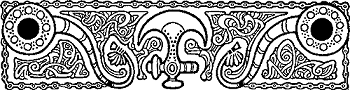
\includegraphics[width=9.3cm]{viking-tales/009}\\
    The Baby}

\lettrine{K}{ing Halfdan} lived in Norway long ago. One morning his
queen said to him:
\vskip\baselineskip
``I had a strange dream last night. I thought that I stood in the grass
before my bower.\footnote{See note about house on page~\pageref{house}.}
I pulled a thorn from my dress. As I held it in my fingers, it grew into
a tall tree. The trunk was thick and red as blood, but the lower limbs
were fair and green, and the highest ones were white. I thought that the
branches of this great tree spread so far that they covered all Norway
and even more.''

``A strange dream,'' said King Halfdan. ``Dreams are the messengers of
the gods. I wonder what they would tell us,'' and he stroked his beard
in thought.

Some time after that a serving-woman came into the feast hall where King
Halfdan was. She carried a little white bundle in her arms.

``My lord,'' she said, ``a little son is just born to you.''

``Ha!'' cried the king, and he jumped up from the high seat and hastened
forward until he stood before the woman.

``Show him to me!'' he shouted, and there was joy in his voice.

The serving-woman put down her bundle on the ground and turned back the
cloth. There was a little naked baby. The king looked at it carefully.

``It is a goodly youngster,'' he said, and smiled. ``Bring Ivar and
Thorstein.''\footnote{See note about names on page~\pageref{names}.}

They were captains of the king's soldiers. Soon they came.

``Stand as witnesses,'' Halfdan said.

Then he lifted the baby in his arms, while the old serving-woman brought
a silver bowl of water. The king dipped his hand into it and sprinkled
the baby, saying:

``I own this baby for my son. He shall be called Harald. My naming gift
to him is ten pounds of gold.''

Then the woman carried the baby back to the queen's room.

\begin{figure}[ht]
    \centering
    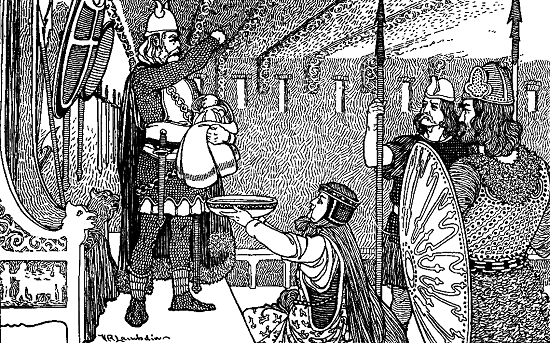
\includegraphics[width=14.6cm]{viking-tales/010}
    \caption{``I own this baby for my son. He shall be called Harald''}
\end{figure}

``My lord owns him for his son,'' she said. ``And no wonder! He is
perfect in every limb.''

The queen looked at him and smiled and remembered her dream and thought:

``That great tree! Can it be this little baby of mine?''

\begin{figure}[hb]
    \centering
    \vskip8pt
    
\includegraphics[width=2.7cm]{viking-tales/011}
\end{figure}

    \chapter[The Tooth Thrall]{
    
\includegraphics[width=9.3cm]{viking-tales/012}\\
    The Tooth Thrall}

\lettrine{W}{hen} Harald was seven months old he cut his first tooth.
Then his father said:
\vskip\baselineskip
``All the young of my herds, lambs and calves and colts, that have been
born since this baby was born I this day give to him. I also give to him
this thrall, Olaf. These are my tooth-gifts to my son.''

The boy grew fast, for as soon as he could walk about he was out of
doors most of the time. He ran in the woods and climbed the hills and
waded in the creek. He was much with his tooth thrall, for the king had
said to Olaf:

``Be ever at his call.''

Now this Olaf was full of stories, and Harald liked to hear them.

``Come out to Aegir's Rock, Olaf, and tell me stories,'' he said almost
every day.

So they started off across the hills. The man wore a long, loose coat of
white wool, belted at the waist with a strap. He had on coarse shoes and
leather leggings. Around his neck was an iron collar welded together so
that it could not come off. On it were strange marks, called runes, that
said:

``Olaf, thrall of Halfdan.''

But Harald's clothes were gay. A cape of gray velvet hung from his
shoulders. It was fastened over his breast with great gold buckles. When
it waved in the wind, a scarlet lining flashed out, and the bottom of a
little scarlet jacket showed. His feet and legs were covered with gray
woolen tights. Gold lacings wound around his legs from his shoes to his
knees. A band of gold held down his long, yellow hair.

It was a wild country that these two were walking over. They were
climbing steep, rough hills. Some of them seemed made all of rock, with
a little earth lying in spots. Great rocks hung out from them, with
trees growing in their cracks. Some big pieces had broken off and rolled
down the hill.

``Thor broke them,'' Olaf said. ``He rides through the sky and hurls his
hammer at clouds and at mountains. That makes the thunder and the
lightning and cracks the hills. His hammer never misses its aim, and it
always comes back to his hand and is eager to go again.''

When they reached the top of the hill they looked back. Far below was a
soft, green valley. In front of it the sea came up into the land and
made a fiord. On each side of the fiord high walls of rock stood up and
made the water black with shadow. All around the valley were high hills
with dark pines on them. Far off were the mountains. In the valley were
Halfdan's houses around their square yard.

``How little our houses look down there!'' Harald said. ``But I can
almost--yes, I can see the red dragon on the roof of the feast hall. Do
you remember when I climbed up and sat on his head, Olaf?''

He laughed and kicked his heels and ran on.

\begin{figure}
    \centering
    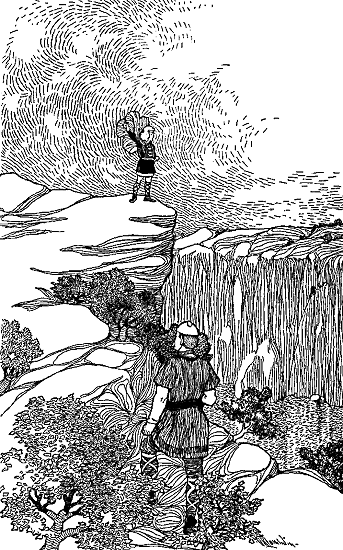
\includegraphics[width=9.1cm]{viking-tales/013}
    \caption{
        ``He threw back his cape and drew a little dagger from his
        belt''}
\end{figure}

At last they came to Aegir's Rock and walked up on its flat top. Harald
went to the edge and looked over. A ragged wall of rock reached down,
and two hundred feet below was the black water of the fiord. Olaf
watched him for a while, then he said:

``No whitening of your cheek, Harald? Good! A boy that can face the fall
of Aegir's Rock will not be afraid to face the war flash when he is a
man.''

``Ho, I am not afraid of the war flash now,'' cried Harald.

He threw back his cape and drew a little dagger from his belt.

``See!'' he cried; ``does this not flash like a sword? And I am not
afraid. But after all, this is a baby thing! When I am eight years old I
will have a sword, a sharp tooth of war.''

He swung his dagger as though it were a long sword. Then he ran and sat
on a rock by Olaf.

``Why is this Aegir's Rock?'' he asked.

``You know that Asgard is up in the sky,'' Olaf said. ``It is a wonderful
city where the golden houses of the gods are in the golden grove. A high
wall runs all around it. In the house of Odin, the All-father, there is
a great feast hall larger than the whole earth. Its name is Valhalla. It
has five hundred doors. The rafters are spears. The roof is thatched
with shields. Armor lies on the benches. In the high seat sits Odin, a
golden helmet on his head, a spear in his hand. Two wolves lie at his
feet. At his right hand and his left sit all the gods and goddesses, and
around the hall sit thousands and thousands of men, all the brave ones
that have ever died.

``Now it is good to be in Valhalla; for there is mead there better than
men can brew, and it never runs out. And there are skalds that sing
wonderful songs that men never heard. And before the doors of Valhalla
is a great meadow where the warriors fight every day and get glorious
and sweet wounds and give many. And all night they feast, and their
wounds heal. But none may go to Valhalla except warriors that have died
bravely in battle. Men who die from sickness go with women and children
and cowards to Niflheim. There Hela, who is queen, always sneers at
them, and a terrible cold takes hold of their bones, and they sit down
and freeze.

``Years ago Aegir was a great warrior. Aegir the Big-handed, they called
him. In many a battle his sword had sung, and he had sent many warriors
to Valhalla. Many swords had bit into his flesh and left marks there,
but never a one had struck him to death. So his hair grew white and his
arms thin. There was peace in that country then, and Aegir sorrowed,
saying:

`\,``I am old. Battles are still. Must I die in bed like a woman? Shall I
not see Valhalla?'

``Now thus did Odin say long ago:

`\,``If a man is old and is come near death and cannot die in fight, let
him find death in some brave way and he shall feast with me in
Valhalla.'

``So one day Aegir came to this rock.

`\,``A deed to win Valhalla!' he cried.

``Then he drew his sword and flashed it over his head and held his
shield high above him, and leaped out into the air and died in the water
of the fiord.''

``Ho!'' cried Harald, jumping to his feet. ``I think that Odin stood up
before his high seat and welcomed that man gladly when he walked through
the door of Valhalla.''

``So the songs say,'' replied Olaf, ``for skalds still sing of that deed
all over Norway.''

\begin{figure}[hb]
    \centering
    \vskip8pt
    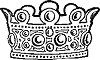
\includegraphics[width=2.7cm]{viking-tales/014}
\end{figure}

    \chapter[Olaf's Farm]{
    
\includegraphics[width=9.3cm]{viking-tales/015}\\
    Olaf's Farm}

\lettrine{A}{t} another time Harald asked:
\vskip2\baselineskip
``What is your country, Olaf? Have you always been a thrall?''

The thrall's eyes flashed.

``When you are a man,'' he said, ``and go a-viking to Denmark, ask men
whether they ever heard of Olaf the Crafty. There, far off, is my
country, across the water. My father was Gudbrand the Big. Two hundred
warriors feasted in his hall and followed him to battle. Ten sons sat at
meat with him, and I was the youngest. One day he said:

`\,``You are all grown to be men. There is not elbow-room here for so many
chiefs. The eldest of you shall have my farm when I die. The rest of
you, off a-viking!'

``He had three ships. These he gave to three of my brothers. But I stayed
that spring and built me a boat. I made her for only twenty oars because
I thought few men would follow me; for I was young, fifteen years old. I
made her in the likeness of a dragon. At the prow I carved the head with
open mouth and forked tongue thrust out. I painted the eyes red for
anger.

`\,``There, stand so!' I said, `and glare and hiss at my foes.'

``In the stern I curved the tail up almost as high as the head. There I
put the pilot's seat and a strong tiller for the rudder. On the breast
and sides I carved the dragon's scales. Then I painted it all black and
on the tip of every scale I put gold. I called her `Waverunner.' There
she sat on the rollers, as fair a ship as I ever saw.

``The night that it was finished I went to my father's feast. After the
meats were eaten and the mead-horns came round, I stood up from my bench
and raised my drinking-horn\footnote{See note about drinking-horns on
page~\pageref{drinking-horns}.} high and spoke with a great voice:

`\,``This is my vow: I will sail to Norway and I will harry the coast and
fill my boat with riches. Then I will get me a farm and will winter in
that land. Now who will follow me?'

`\,``He is but a boy,' the men said. `He has opened his mouth wider than he
can do.'

``But others jumped to their feet with their mead-horns in their hands.
Thirty men, one after another, raised their horns and said:

`\,``I will follow this lad, and I will not turn back so long as he and I
live!'

``On the next morning we got into my dragon and started. I sat high in
the pilot's seat. As our boat flashed down the rollers into the water I
made this song and sang it:

\begin{quote}
`\,``The dragon runs.\\
Where will she steer?\\
Where swords will sing,\\
Where spears will bite,\\
Where I shall laugh.'
\end{quote}

``So we harried the coast of Norway. We ate at many men's tables
uninvited. Many men we found overburdened with gold. Then I said:

`\,``My dragon's belly is never full,' and on board went the gold.

``Oh! it is better to live on the sea and let other men raise your crops
and cook your meals. A house smells of smoke, a ship smells of frolic.
From a house you see a sooty roof, from a ship you see Valhalla.

``Up and down the water we went to get much wealth and much frolic. After
a while my men said:

`\,``What of the farm, Olaf?'

`\,``Not yet,' I answered. `Viking is better for summer. When the ice
comes, and our dragon cannot play, then we will get our farm and sit
down.'

``At last the winter came, and I said to my men:

`\,``Now for the farm. I have my eye on one up the coast a way in King
Halfdan's country.'

``So we set off for it. We landed late at night and pulled our boat up on
shore and walked quietly to the house. It was rather a wealthy farm, for
there were stables and a storehouse and a smithy at the sides of the
house. There was but one door to the house. We went to it, and I struck
it with my spear.

\begin{figure}
    \centering
    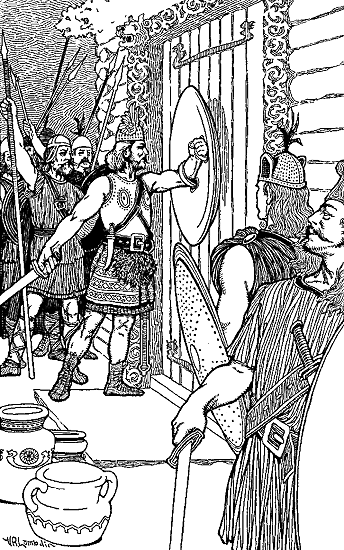
\includegraphics[width=9.1cm]{viking-tales/016}
    \caption{
        ``I struck my shield against the door so that it made a great
        clanging''}
\end{figure}

`\,``Hello! Ho! Hello!' I shouted, and my men made a great din.

``At last some one from inside said:

`\,``Who calls?'

`\,``I call,' I answered. `Open! or you will think it Thor who calls,' and
I struck my shield against the door so that it made a great clanging.

``The door opened only a little, but I pushed it wide and leaped into the
room. It was so dark that I could see nothing but a few sparks on the
hearth. I stood with my back to the wall; for I wanted no sword reaching
out of the dark for me.

`\,``Now start up the fire,' I said.

`\,``Come, come!' I called, when no one obeyed. `A fire! This is cold
welcome for your guests.'

``My men laughed.

`\,``Yes, a stingy host! He acts as though he had not expected us.'

``But now the farmer was blowing on the coals and putting on fresh wood.
Soon it blazed up, and we could see about us. We were in a little feast
hall,\footnote{See note about feast hall on page~\pageref{feast-hall}.}
with its fire down the middle of it. There were benches for twenty men
along each side. The farmer crouched by the fire, afraid to move. On a
bench in a far corner were a dozen people huddled together.

`\,``Ho, thralls!' I called to them. `Bring in the table. We are hungry.'

``Off they ran through a door at the back of the hall. My men came in and
lay down by the fire and warmed themselves, but I set two of them as
guards at the door.

`\,``Well, friend farmer,' laughed one, `why such a long face? Do you not
think we shall be merry company?'

`\,``We came only to cheer you,' said another. `What man wants to spend the
winter with no guests?'

`\,``Ah!' another then cried out, sitting up. `Here comes something that
will be a welcome guest to my stomach.'

``The thralls were bringing in a great pot of meat. They set up a crane
over the fire and hung the pot upon it, and we sat and watched it boil
while we joked. At last the supper began. The farmer sat gloomily on the
bench and would not eat, and you cannot wonder; for he saw us putting
potfuls of his good beef and basket-loads of bread into our big mouths.
When the tables were taken out and the mead-horns came round, I stood up
and raised my horn and said to the farmer:

`\,``You would not eat with us. You cannot say no to half of my ale. I
drink this to your health.'

``Then I drank half of the hornful and sent the rest across the fire to
the farmer. He took it and smiled, saying:

`\,``Since it is to my health, I will drink it. I thought that all this
night's work would be my death.'

`\,``Oh, do not fear that!' I laughed, `for a dead man sets no tables.'

``So we drank and all grew merrier. At last I stood up and said:

`\,``I like this little taste of your hospitality, friend farmer. I have
decided to accept more of it.'

``My men roared with laughter.

`\,``Come,' they cried, `thank him for that, farmer. Did you ever have such
a lordly guest before?'

``I went on:

`\,``Now there is no fun in having guests unless they keep you company and
make you merry. So I will give out this law: that my men shall never
leave you alone. Hakon there shall be your constant companion, friend
farmer. He shall not leave you day or night, whether you are working or
playing or sleeping. Leif and Grim shall be the same kind of friends to
your two sons.'

``I named nine others and said:

`\,``And these shall follow your thralls in the same way. Now, am I not
careful to make your time go merrily?'

``So I set guards over every one in that house. Not once all that winter
did they stir out of sight of some of us. So no tales got out to the
neighbors. Besides, it was a lonely place, and by good luck no one came
that way. Oh! that was fat and easy living.

``Well, after we had been there for a long time, Hakon came in to the
feast one night and said:

`\,``I heard a cuckoo to-day!'

`\,``It is the call to go a-viking,' I said.

``All my men put their hands to their mouths and shouted. Their eyes
danced. Big Thorleif stood up and stretched himself.

`\,``I am stiff with long sitting,' he said. `I itch for a fight.'

``I turned to the farmer.

`\,``This is our last feast with you,' I said.

`\,``Well,' he laughed, `this has been the busiest winter I ever spent, and
the merriest. May good luck go with you!'

`\,``By the beard of Odin!' I cried; `you have taken our joke like a man.'

``My men pounded the table with their fists.

`\,``By the hammer of Thor!' shouted Grim. `Here is no stingy coward. He is
a man fit to carry my drinking-horn, the horn of a sea-rover and a
sword-swinger. Here, friend, take it,' and he thrust it into the
farmer's hand. `May you drink heart's-ease from it for many years. And
with it I leave you a name, Sif the Friendly. I shall hope to drink with
you sometime in Valhalla.'

``Then all my men poured around that farmer and clapped him on the
shoulder and piled things upon him, saying:

`\,``Here is a ring for Sif the Friendly.'

`\,``And here is a bracelet.'

`\,``A sword would not be ashamed to hang at your side.'

``I took five great bracelets of gold from our treasure chest and gave
them to him.

``The old man's eyes opened wide at all these things, and at the same
time he laughed.

`\,``May Odin send me such guests every winter!' he said.

``Early next morning we shook hands with our host and boarded the
`Waverunner' and sailed off.

`\,``Where shall we go?' my men asked.

`\,``Let the gods decide,' I said, and tossed up my spear.

``When it fell on the deck it pointed up-shore, so I steered in that
direction. That is the best way to decide, for the spear will always
point somewhere, and one thing is as good as another. That time it
pointed us into your father's ships. They closed in battle with us and
killed my men and sunk my ship and dragged me off a prisoner. They were
three against one, or they might have tasted something more bitter at
our hands. They took me before King Halfdan.

`\,``Here,' they said, `is a rascal who has been harrying our coasts. We
sunk his ship and men, but him we brought to you.'

`\,``A robber viking?' said the king, and scowled at me.

``I threw back my head and laughed.

`\,``Yes. And with all your fingers it took you a year to catch me.'

``The king frowned more angrily.

`\,``Saucy, too?' he said. `Well, thieves must die. Take him out, Thorkel,
and let him taste your sword.'

``Your mother, the queen, was standing by. Now she put her hand on his
arm and smiled and said:

`\,``He is only a lad. Let him live. And would he not be a good gift for
our baby?'

``Your father thought a moment, then looked at your mother and smiled.

`\,``Soft heart!' he said gently to her; then to Thorkel, `Well, let him
go, Thorkel!'

``Then he turned to me again, frowning.

`\,``But, young sharp-tongue, now that we have caught you we will put you
into a trap that you cannot get out of. Weld an iron collar on his
neck.'

``So I lived and now am your tooth thrall. Well, it is the luck of war.
But by the chair of Odin, I kept my vow!''

``Yes!'' cried Harald, jumping to his feet. ``And had a joke into the
bargain. Ah! sometime I will make a brave vow like that.''

\begin{figure}[hb]
    \centering
    \vskip8pt
    
\includegraphics[width=2.7cm]{viking-tales/017}
\end{figure}

    \section[Olaf's Fight with Havard]{
    
\includegraphics[width=9.3cm]{viking-tales/018}\\
    Olaf's Fight with Havard}

\lettrine{A}{t} another time Harald said:
\vskip2\baselineskip
``Tell me of a fight, Olaf. I want to hear about the music of swords.''

Olaf's eyes blazed.

``I will tell you of our fight with King Havard,'' he said.

``One dark night we had landed at a farm. We left our `Waverunner' in the
water with three men to guard her. The rest of us went into the house.
The farmer met us at the door, but he died by Thorkel's sword. The
others we shut into their beds.\footnote{See note about beds on
page~\pageref{beds}.} The door at each end of the hall we had barred on
the inside so that nobody could surprise us. We were busy going through
the cupboards and shouting at our good luck. But suddenly we heard a
shout outside:

```Thor and Havard!'

``Then there was a great beating at the doors.

```He has two hundred fighters with him,' said Grim; `for we saw his
ships last night. Thirty against two hundred! We shall all drink in
Valhalla to-night.'

```Well,' I cried, `Odin shall have no unwilling guest in me.'

```Nor in me,' cried Hakon.

```Nor in me,' shouted Thorkel.

``And that shout went all around, and we drew out our swords and caught
up our shields.

```Hot work is ahead of us,' said Hakon. `Besides, we must leave none of
this mead for Havard. Lend a hand, some one.'

``Then he and another pulled out a great tub that sat on the floor of the
cupboard.

```I drink to Valhalla to-night,' cried Thorkel the Thirsty, and he
plunged his horn deep into the tub.

``When he brought it up, his sleeve was dripping and the sweet mead was
running over from the horn.

```Sloven!' cried Hakon, and he struck Thorkel with his fist and knocked
him over into the cupboard.

``He fell against the wooden wall at the back, and a carved panel swung
open behind him. He dropped down head first. In a minute he put his head
out of the hole again. We all stood staring.

```I think it is a secret passage,' he said.

```We will try it,' I answered in a whisper. `Throw dirt on the fire. It
must be dark.'

``So we dug up dirt from the earth floor and smothered the fire. All this
time there was a terrible shouting and hammering at the doors, but they
were of heavy logs and stood.

```I with four more will guard this door,' I said, pointing to the east
end.

``Immediately four men stepped to my side.

```And I will guard the other,' Hakon said, and four went with him.

```The rest of you, down the hole!' I said. `Close the door after you. If
luck is with us we will meet at the ships. Now Thor and our good swords
help us! Quick! The doors are giving way.'

``So we ten men stood at the doors and held back the king's soldiers. It
was dark in the room, and the people out of doors could not tell how
many were inside. Few were eager to be the first in.

```Thirty swords are waiting in there to eat up the first man,' we heard
some one say.

``We chuckled at that.

``But the king stood in the very doorway and fought. Our five swords held
him back for a long time, but at last he pushed in, and his men poured
after him. We ran back and hid behind some tubs in a dark corner. The
king's men went groping about and calling, but they did not find us. The
room was full of shouting and running and sword-clashing; for in the
dark and the noise the men could not tell their own soldiers. More than
one fell by his friend's sword. When it was less crowded about the
doorway, I whispered:

```Follow me in double line. We will make for the ships. Keep close
together.'

``So that double line of men, with swords swinging from both sides, ran
out through the dark. Swords struck out at us, and we struck back. Men
ran after us shouting, but our legs were as good as theirs. But I and
Hakon and one other were all that reached the ship. There we saw our
`Waverunner' with sail up and bow pointing to open sea. We swam out to
her and climbed aboard. Then the men swung the sail to the wind, and we
moved off. Even as we went, a spear whizzed through the air, and Hakon
fell dead; for the king and all his men were running to the shore.

```After them!' they were shouting.

``Then we heard the king call to the men in his boats lying out in the
water:

```Row to shore and take us in.'

``Thorkel was standing by my side. At that he laughed and said:

```They do not answer. He left but a handful to guard his ships. They
tasted our swords. And we went aboard and broke the oars and threw the
sails into the water. It will be slow going for Havard to-night.'

\begin{figure}
    \centering
    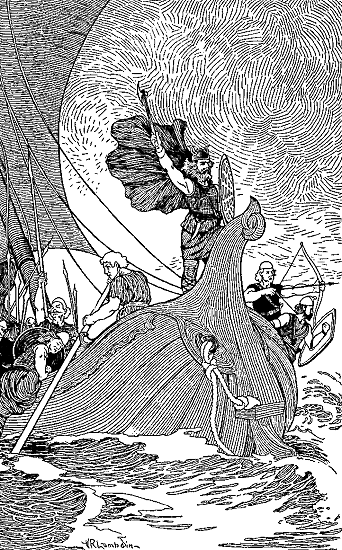
\includegraphics[width=9.1cm]{viking-tales/019}
    \caption{``Then he turned to the shore and sang out loudly''}
\end{figure}

``Then he turned to the shore and sang out loudly:

\begin{quote}
```King Havard's ships are dead:\\
Olaf's dragon flies.\\
King Havard stamps the shore:\\
Olaf skims the waves.\\
King Havard shakes his fist.\\
Olaf turns and laughs.'
\end{quote}

``That was the end of our meeting with King Havard.''

\begin{figure}
    \centering
    \vskip8pt
    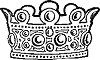
\includegraphics[width=2.7cm]{viking-tales/014}
\end{figure}

    \chapter[Foes'-fear]{
    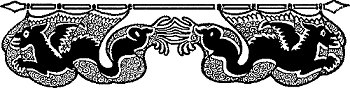
\includegraphics[width=9.3cm]{viking-tales/020}\\
    Foes'-fear}

\lettrine{E}{very} day the boy Harald heard some such story of war or of
the gods, until he could see Thor riding among the storm-clouds and
throwing his hammer, until he knew that a brave man has many wounds, but
never a one on his back. Many nights he dreamed that he himself walked
into Valhalla, and that all the heroes stood up and shouted:

``Welcome! Harald Halfdanson!''

``Ah! the bite of the sword is sweeter than the kiss of your mother,''
he said to Olaf one day. ``When shall I stand in the prow of a dragon
and feast on the fight? I am hungry to see the world. Ivar the Far-goer
tells me of the strange countries he has seen. Ah! we vikings are great
folk. There is no water that has not licked our boats' sides. This cape
of mine came in a viking boat from France. These cloak-pins came from a
far country called Greece. In my father's house are golden cups from
Rome, away on the southern sea. Every land pours rich things into our
treasure-chest. Ivar has been to a strange country where it is all sand
and is very hot. The people call their country Arabia. They have never
heard of Thor or Odin. Ivar brought beautiful striped cloth from there,
and wonderful, sweet-smelling waters. Oh! when shall the white horses of
the sea lead me out to strange lands and glorious battles?''

But Harald did something besides listen to stories. Every morning he was
up at sunrise and went with a thrall to feed the hunting dogs. Thorstein
taught him to swim in the rough waters of the fiord. Often he went with
the men a-hunting in the woods and learned to ride a horse and pull a
bow and throw a lance. Ivar taught him to play the harp and to make up
songs. He went much to the smithy, where the warriors mended their
helmets and made their spears and swords of iron and bronze. At first he
only watched the men or worked the bellows, but soon he could handle the
tongs and hold the red-hot iron, and after a long time he learned to use
the hammer and to shape metal. One day he made himself a spear-head. It
was two feet long and sharp on both edges. While the iron was hot he
beat into it some runes. When the men in the smithy saw the runes they
opened their eyes wide and looked at the boy, for few Norsemen could
read.

``What does it say?'' they asked.

``It is the name of my spear-point, and it says, `Foes'-fear,''' Harald
said. ``But now for a handle.''

It was winter and the snow was very deep. So Harald put on his skees and
started for a wood that was back from shore. Down the mountains he went,
twenty, thirty feet at a slide, leaping over chasms a hundred feet
across. In his scarlet cloak he looked like a flash of fire. The wind
shot past him howling. His eyes danced at the fun.

``It is like flying,'' he thought and laughed. ``I am an eagle. Now I
soar,'' as he leaped over a frozen river.

He saw a slender ash growing on top of a high rock.

``That is the handle for `Foes'-fear,''' he said.

The rock stood up like a ragged tower, but he did not stop because of
the steep climb. He threw off his skees and thrust his hands and feet
into holes of the rock and drew himself up. He tore his jacket and cut
his leather leggings and scratched his face and bruised his hands, but
at last he was on the top. Soon he had chopped down the tree and had cut
a straight pole ten feet long and as big around as his arm. He went
down, sliding and jumping and tearing himself on the sharp stones. With
a last leap he landed near his skees. As he did so a lean wolf jumped
and snapped at him, snarling. Harald shouted and swung his pole. The
wolf dodged, but quickly jumped again and caught the boy's arm between
his sharp teeth. Harald thought of the spear-point in his belt. In a
wink he had it out and was striking with it. He drove it into the wolf's
neck and threw him back on the snow, dead.

``You are the first to feel the tooth of `Foes'-fear,''' he said, ``but
I think you will not be the last.''

\begin{figure}
    \centering
    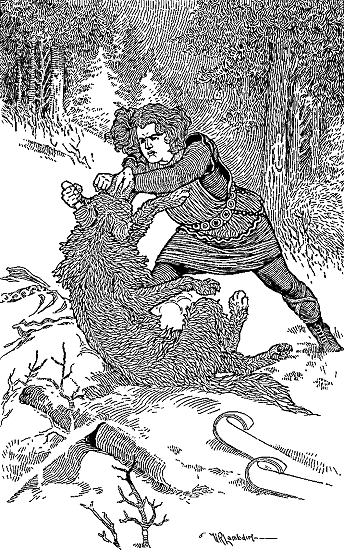
\includegraphics[width=9.1cm]{viking-tales/021}
    \caption{``He drove it into the wolf's neck''}
\end{figure}

Then without thinking of his torn arm he put on his skees and went
leaping home. He went straight to the smithy and smoothed his pole and
drove it into the haft of the spear-point. He hammered out a gold band
and put it around the joining place. He made nails with beautiful heads
and drove them into the pole in different places.

``If it is heavy it will strike hard,'' he said.

Then he weighed the spear in his hand and found the balancing point and
put another gold band there to mark it.

Thorstein came in while he was working.

``A good spear,'' he said.

Then he saw the torn sleeve and the red wound beneath.

``Hello!'' he cried. ``Your first wound?''

``Oh, it is only a wolf-scratch,'' Harald answered.

``By Thor!'' cried Thorstein, ``I see that you are ready for better
wounds. You bear this like a warrior.''

``I think it will not be my last,'' Harald said.

    \section[Harald is King]{
    
\includegraphics[width=9.3cm]{viking-tales/022}\\
    Harald is King}

\lettrine{N}{ow} when Harald was ten years old his father, King Halfdan,
died. An old book that tells about Harald says that then ``he was the
biggest of all men, the strongest, and the fairest to look upon.'' That
about a boy ten years old! But boys grew fast in those days for they were
out of doors all the time, running, swimming, leaping on skees, and
hunting in the forest. All that makes big, manly boys.

So now King Halfdan was dead and buried, and Harald was to be king. But
first he must drink his father's funeral ale.

``Take down the gay tapestries that hang in the feast hall,'' he said to
the thralls. ``Put up black and gray ones. Strew the floor with pine
branches. Brew twenty tubs of fresh ale and mead. Scour every dish until
it shines.''

Then Harald sent messengers all over that country to his kinsmen and
friends.

``Bid them come in three months' time to drink my father's funeral
ale,'' he said. ``Tell them that no one shall go away empty-handed.''

So in three months men came riding up at every hour. Some came in boats.
But many had ridden far through mountains, swimming rivers; for there
were few roads or bridges in Norway. On account of that hard ride no
women came to the feast.

At nine o'clock in the night the feast began. The men came walking in at
the west end of the hall.\footnote{See note about feast hall on
page~\pageref{feast-hall}.} The great bonfires down the middle of the
room were flashing light on everything. The clean smell of this
wood-smoke and of the pine branches on the floor was pleasant to the
guests. Down each side of the hall stretched long, backless benches, with
room for three hundred men. In the middle of each side rose the high
seat, a great carved chair on a platform. All along behind the benches
were the black and gray draperies. Here hung the shields of the guests;
for every man, when he was given his place, turned and hung his shield
behind him and set his tall spear by it. So on each wall there was a long
row of gay shields, red and green and yellow, and all shining with gold
or bronze trimmings. And higher up there was another row of gleaming
spear-points. Above the hall the rafters were carved and gaily painted,
so that dragons seemed to be crawling across, or eagles seemed to be
swooping down.

The guests walked in laughing and talking with their big voices so that
the rafters rang. They made the hall look all the brighter with their
clothes of scarlet and blue and green, with their flashing golden
bracelets and head-bands and sword-scabbards, with their flying hair of
red or yellow.

Across the east end of the hall was a bench. When the men were all in,
the queen, Harald's mother, and the women who lived with her, walked in
through the east door and sat upon this bench.

Then thralls came running in and set up the long tables\footnote{See note
about tables on page~\pageref{tables}.} before the benches. Other thralls
ran in with large steaming kettles of meat. They put big pieces of this
meat into platters of wood and set it before the men. They had a few
dishes of silver. These they put before the guests at the middle of the
tables; for the great people sat here near the high seats.

When the meat came, the talking stopped; for Norsemen ate only twice a
day, and these men had had long rides and were hungry. Three or four
persons ate from one platter and drank from the same big bowl of milk.
They had no forks, so they ate from their fingers and threw the bones
under the table among the pine branches. Sometimes they took knives from
their belts to cut the meat.

When the guests sat back satisfied, Harald called to the thralls:

``Carry out the tables.''

So they did and brought in two great tubs of mead and set one at each
end of the hall. Then the queen stood up and called some of her women.
They went to the mead tubs. They took the horns, when the thralls had
filled them, and carried them to the men with some merry word. Perhaps
one woman said as she handed a man his horn:

``This horn has no feet to be set down upon. You must drink it at one
draught.''

Perhaps another said:

``Mead loves a merry face.''

The women were beautiful, moving about the hall. The queen wore a
trailing dress of blue velvet with long flowing sleeves. She had a short
apron of striped Arabian silk with gold fringe along the bottom. From
her shoulders hung a long train of scarlet wool embroidered in gold.
White linen covered her head. Her long yellow hair was pulled around at
the sides and over her breast and was fastened under the belt of her
apron. As she walked, her train made a pleasant rustle among the pine
branches. She was tall and straight and strong. Some of her younger
women wore no linen on their heads and had their white arms bare, with
bracelets shining on them. They, too, were tall and strong.

All the time men were calling across the fire to one another asking news
or telling jokes and laughing.

An old man, Harald's uncle, sat in the high seat on the north side. That
was the place of honor. But the high seat on the south side was empty;
for that was the king's seat. Harald sat on the steps before it.

The feast went merrily until long after midnight. Then the thralls took
some of the guests to the guest house to sleep, and some to the beds
around the sides of the feast hall. But some men lay down on the benches
and drew their cloaks over themselves.

On the next night there was another feast. Still Harald sat on the step
before the high seat. But when the tables were gone and the horns were
going around, he stood up and raised high a horn of ale and said loudly:

``This horn of memory I drink in honor of my father, Halfdan, son of
Gudrod, who sits now in Valhalla. And I vow that I will grind my
father's foes under my heel.''

Then he drank the ale and sat down in the king's high seat, while all
the men stood up and raised their horns and shouted:

``King Harald!''

And some cried:

``That was a brave vow.''

\begin{figure}
    \centering
    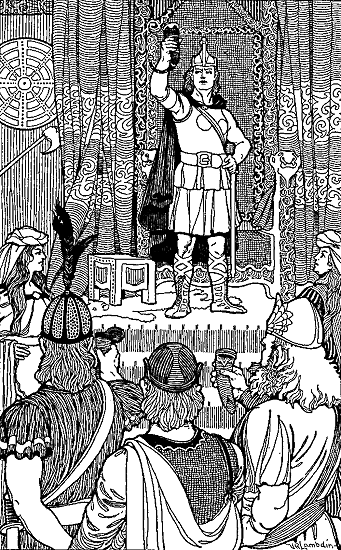
\includegraphics[width=9.1cm]{viking-tales/023}
    \caption{``I vow that I will grind my father's foes under my heel''}
\end{figure}

And Harald's uncle called out:

``A health to King Harald!''

And they all drank it.

Then a man stood up and said:

``Hear my song of King Halfdan!'' for this man was a skald.

``Yes, the song!'' shouted the men, and Harald nodded his head.

So the skald took down his great harp from the wall behind him and went
and stood before Harald. The bottom of the harp rested on the floor, but
the top reached as high as the skald's shoulders. The brass frame shone
in the light. The strings were some of gold and some of silver. The man
struck them with his hand and sang of King Halfdan, of his battles, of
his strong arm and good sword, of his death, and of how men loved him.

When he had finished, King Harald took a bracelet from his arm and gave
it to him, saying:

``Take this as thanks for your good song.''

The guests stayed the next day and at night there was another feast.
When the mead horns were going around, King Harald stood up and spoke:

``I said that no man should go away empty-handed from drinking my
father's funeral ale.''

He beckoned the thralls, and they brought in a great treasure-chest and
set it down by the high seat. King Harald opened it and took out rich
gifts--capes and sword-belts and beautiful cloth and bracelets and gold
cloak-pins. These he sent about the hall and gave something to every
man. The guests wondered at the richness of his gifts.

``This young king has an open hand,'' they said, ``and deep
treasure-chests.''

After breakfast the next morning the guests went out and stood by their
horses ready to go, but before they mounted, thralls brought a horn of
mead to each man. That was called the stirrup-horn, because after they
drank it the men put their feet to the stirrups and sprang upon their
horses and started. King Harald and his people rode a little way with
them.

All men said that that was the richest funeral feast that ever was held.

    \section[Harald's Battle]{
    
\includegraphics[width=9.3cm]{viking-tales/024}\\
    Harald's Battle}

\lettrine{N}{ow} King Halfdan had many foes. When he was alive they were
afraid to make war upon him, for he was a mighty warrior. But when Harald
became king, they said:

``He is but a lad. We will fight with him and take his land.''

So they began to make ready. King Harald heard of this and he laughed
and said:

``Good! `Foes'-fear' is thirsty, and my legs are stiff with much
sitting.''

He called three men to him. To one he gave an arrow, saying:

``Run and carry this arrow north. Give it into the hands of the master
of the next farm, and say that all men are to meet here within two weeks
from this day. They must come ready for war and mounted on horses. Say
also that if a man does not obey this call, or if he receives this arrow
and does not carry it on to his next neighbor, he shall be outlawed from
this country, and his land shall be taken from him.''

He gave arrows to the other two men and told them to run south and east
with the same message.

So all through King Harald's country men were soon busy mending helmets
and polishing swords and making shields. There was blazing of forges and
clanging of anvils all through the land.

On the day set, the fields about King Harald's house were full of men
and horses. After breakfast a horn blew. Every man snatched his weapons
and jumped upon his horse. Men of the same neighborhood stood together,
and their chief led them. They waited for the starting horn. This did
not look like our army. There were no uniforms. Some men wore helmets,
some did not. Some wore coats of mail, but others wore only their
jackets and tights of bright-colored wool. But at each man's left side
hung a great shield. Over his right shoulder went his sword-belt and
held his long sword under his left hand. Above most men's heads shone
the points of their tall spears. Some men carried axes in their belts.
Some carried bows and arrows. Many had ram's horns hanging from their
necks.

King Harald rode at the front of his army with his standard-bearer
beside him. Chain-armor covered the king's body. A red cloak was thrown
over his shoulders. On his head was a gold helmet with a dragon standing
up from it. He carried a round shield on his left arm. The king had made
that shield himself. It was of brass. The rivets were of silver, with
strangely shaped heads. On the back of Harald's horse was a red cloth
trimmed with the fur of ermine.

King Harald looked up at his standard and laughed aloud.

``Oh, War-lover,'' he cried, ``you and I ride out on a gay journey.''

A horn blew again and the army started. The men shouted as they went,
and blew their ram's horns.

``Now we shall taste something better than even King Harald's ale,''
shouted one.

Another rose in his stirrups and sniffed the air.

``Ah! I smell a battle,'' he cried. ``It is sweeter than those strange
waters of Arabia.''

So the army went merrily through the land. They carried no tents, they
had no provision wagons.

``The sky is a good enough tent for a soldier,'' said the Norsemen.
``Why carry provisions when they lie in the farms beside you?''

After two days King Harald saw another army on the hills.

``Thorstein,'' he shouted, ``up with the white shield and go tell King
Haki to choose his battle-field. We will wait but an hour. I am eager
for the frolic.''

So Thorstein raised a white shield on his spear as a sign that he came
on an errand of peace. He rode near King Haki, but he could not wait
until he came close before he shouted out his message and then turned
and rode back.

``Tell your boy king that we will not hang back,'' Haki called after
Thorstein.

King Harald's men waited on the hillside and watched the other army
across the valley. They saw King Haki point and saw twenty men ride off
as he pointed. They stopped in a patch of hazel and hewed with their
axes.

``They are getting the hazels,'' said Thorstein.

``Audun,'' said King Harald to a man near him, ``stay close to my
standard all day. You must see the best of the fight. I want to hear a
song about it after it is over.''

This Audun was the skald who sang at the drinking of King Halfdan's
funeral ale.

King Haki's men rode down into the valley. They drove down stakes all
about a great field. They tied the hazel twigs to the stakes in a
string. But they left an open space toward King Harald's army and one
toward King Haki's. Then a man raised a white shield and galloped toward
King Harald.

``We are ready!'' he shouted.

At the same time King Haki raised a red shield. King Harald's men put
their shields before their mouths and shouted into them. It made a great
roaring war-cry.

``Up with the war shield!'' shouted King Harald. ``Horns blow!''

There was a blowing of horns on both sides. The two armies galloped down
into the field and ran together. The fight had begun.

All that day long swords were flashing, spears flying, men shouting, men
falling from their horses, swords clashing against shields.

``Victory flashes from that dragon,'' Harald's men said, pointing to the
king's helmet. ``No one stands before it.''

And, surely, before night came, King Haki fell dead under
``Foes'-fear.'' When he fell, a great shout went up from his warriors,
and they turned and fled. King Harald's men chased them far, but during
the night came back to camp. Many brought swords and helmets and
bracelets or silver-trimmed saddles and bridles with them.

``Here is what we got from the foe,'' they said.

The next morning King Harald spoke to his men:

``Let us go about and find our dead.''

\begin{figure}
    \centering
    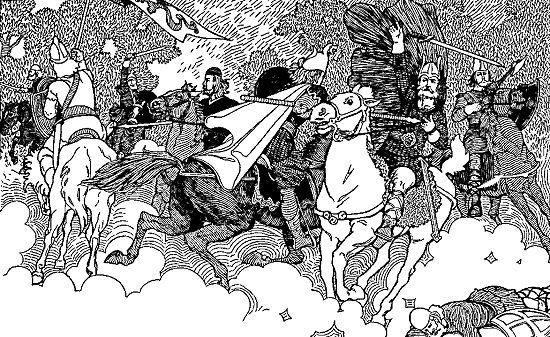
\includegraphics[width=14.6cm]{viking-tales/025}
    \caption{``King Haki fell dead under `Foes'-fear'''}
\end{figure}

So they went over all the battle-field. They put every man on his shield
and carried him and laid him on a hill-top. They hung his sword over his
shoulder and laid his spear by his side. So they laid all the dead
together there on the hill-top. Then King Harald said, looking about:

``This is a good place to lie. It looks far over the country. The sound
of the sea reaches it. The wind sweeps here. It is a good grave for
Norsemen and Vikings. But it is a long road and a rough road to Valhalla
that these men must travel. Let the nearest kinsman of each man come and
tie on his hell-shoes. Tie them fast, for they will need them much on
that hard road.''

So friends tied shoes on the dead men's feet. Then King Harald said:

``Now let us make the mound.''

Every man set to work with what tools he had and heaped earth over the
dead until a great mound stood up. They piled stones on the top. On one
of these stones King Harald made runes telling how these men had died.

After that was done King Harald said:

``Now set up the pole, Thorstein. Let every man bring to that pole all
that he took from the foe.''

So they did, and there was a great hill of things around it. Harald
divided it into piles.

``This pile we will give to Thor in thanks for the victory,'' he said.
``This pile is mine because I am king. Here are the piles for the
chiefs, and these things go to the other men of the army.''

So every man went away from that battle richer than he was before, and
Thor looked down from Valhalla upon his full temple and was pleased.

The next morning King Harald led his army back. But on the way he met
other foes and had many battles and did not lose one. The kings either
died in battle or ran away, and Harald had their lands.

``He has kept his vow,'' men said, ``and ground his father's foes under
his heel.''

So King Harald sat in peace for a while.

    \chapter[Gyda's Saucy Message]{
    
\includegraphics[width=9.3cm]{viking-tales/026}\\
    Gyda's Saucy Message}

\lettrine{N}{ow} Harald heard men talk of Gyda, the daughter of King
Eric.
\vskip2\baselineskip
``She is very beautiful,'' they said, ``but she is very proud, too. She
can both read and make runes. No other woman in the world knows so much
about herbs as she does. She can cure any sickness. And she is proud of
all this!''

Now when King Harald heard that, he thought to himself:

``Fair and proud. I like them both. I will have her for my wife.''

So he called his uncle, Guthorm, and said:

``Take rich gifts and go to Gyda's foster-father\footnote{See note about
foster-father on page~\pageref{foster-father}.} and tell him that I will
marry Gyda.''

So Guthorm and his men came to that house and they told the king's
message to the foster-father. Gyda was standing near, weaving a rich
cloak. She heard the speech. She came up and said, holding her head high
and curling her lip:

``I will not waste myself on a king of so few people. Norway is a
strange country. There is a little king here and a little king
there--hundreds of them scattered about. Now in Denmark there is but one
great king over the whole land. And it is so in Sweden. Is no one brave
enough to make all of Norway his own?''

She laughed a scornful laugh and walked away. The men stood with open
mouths and stared after her. Could it be that she had sent that saucy
message to King Harald? They looked at her foster-father. He was
chuckling in his beard and said nothing to them. They started out of the
house in anger. When they were at the door, Gyda came up to them again
and said:

``Give this message to your King Harald for me: I will not be his wife
unless he puts all of Norway under him for my sake.''

\begin{figure}[ht]
    \centering
    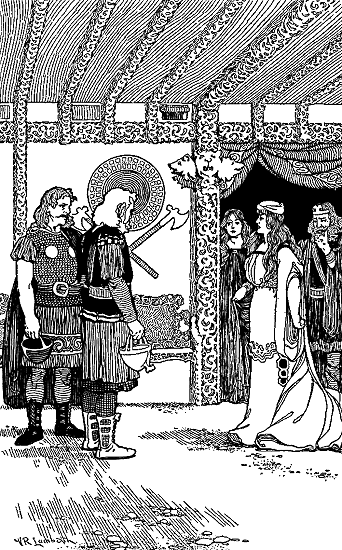
\includegraphics[width=9.1cm]{viking-tales/027}
    \caption{``I will not be his wife unless he puts all of Norway under
        him for my sake''}
\end{figure}

So Guthorm and his men rode homeward across the country. They did not
talk. They were all thinking. At last one said:

``How shall we give this message to the king?''

``I have been thinking of that,'' Guthorm said; ``his anger is no little
thing.''

It was late when they rode into the king's yard; for they had ridden
slowly, trying to make some plan for softening the message, but they had
thought of none.

``I see light through the wind's-eyes of the feast hall,'' one said.

``Yes, the king keeps feast,'' Guthorm said. ``We must give our message
before all his guests.''

So they went in with very heavy hearts. There sat King Harald in the
high seat. The benches on both sides were full of men. The tables had
been taken out, and the mead-horns were going round.

``Oh, ho!'' cried King Harald. ``Our messengers! What news?''

Then Guthorm said:

``This Gyda is a bold and saucy girl, King Harald. My tongue refuses to
give her message.''

The king stamped his foot.

``Out with it!'' he cried. ``What does she say?''

``She says that she will not marry so little a king,'' Guthorm answered.

Harald jumped to his feet. His face flushed red. Guthorm stretched out
his hand.

``They are not my words, O King; they are the words of a silly girl.''

``Is there any more?'' the king shouted. ``Go on!''

``She said: `There is one king in Denmark and one king in Sweden. Is
there no man brave enough to make himself king of all Norway? Tell King
Harald that I will not marry him unless he puts all of Norway under him
for my sake.'\,''

The guests sat speechless, staring at Guthorm. All at once the king
broke into a roar of laughter.

``By the hammer of Thor!'' he cried, ``that is a good message. I thank
you, Gyda. Did you hear it, friends? King of all Norway! Why, we are all
stupids. Why did we not think of that?''

Then he raised his horn high.

``Now hear my vow. I say that I will not cut my hair or comb it until I
am king of all Norway. That I will be or I will die.''

Then he drank off the horn of mead, and while he drank it, all the men
in the hall stood up and waved their swords and shouted and shouted.
That old hall in all its two hundred years of feasts had not heard such
a noise before.

``Ah, Harald!'' Guthorm cried, ``surely Thor in Valhalla smiled when he
heard that vow.''

The men sat all night talking of that wonderful vow.

On the very next day King Harald sent out his war-arrows. Soon a great
army was gathered. They marched through the country north and south and
east and west, burning houses and fighting battles as they went. People
fled before them, some to their own kings, some inland to the deep woods
and hid there. But some went to King Harald and said:

``We will be your men.''

``Then take the oath, and I will be friends with you,'' he said.

The men took off their swords and laid them down and came one by one and
knelt before the king. They put their heads between his knees and said:

``From this day, Harald Halfdanson, I am your man. I will serve you in
war. For my land I will pay you taxes. I will be faithful to you as my
king.''

Then Harald said:

``I am your king, and I will be faithful to you.''

Many kings took that oath and thousands of common men. Of all the
battles that Harald fought, he did not lose one.

Now for a long time the king's hair and beard had not been combed or
cut. They stood out around his head in a great bushy mat of yellow. At a
feast one day when the jokes were going round, Harald's uncle said:

``Harald, I will give you a new name. After this you shall be called
Harald Shockhead. As my naming gift I give you this drinking-horn.''

``It is a good name,'' laughed all the men.

After that all people called him Harald Shockhead.

During these wars, whenever King Harald got a country for his own, this
is what he did. He said:

``All the marshland and the woodland where no people live is mine. For
his farm every man shall pay me taxes.''

Over every country he put some brave, wise man and called him Earl. He
said to the earls:

``You shall collect the taxes and pay them to me. But some you shall
keep for yourselves. You shall punish any man who steals or murders or
does any wicked thing. When your people are in trouble they shall come
to you, and you shall set the thing right. You must keep peace in the
land. I will not have my people troubled with robber vikings.''

The earls did all these things as best they could; for they were good
strong men. The farmers were happy. They said:

``We can work on our farms with peace now. Before King Harald came,
something was always wrong. The vikings would come and steal our gold
and our grain and burn our houses, or the king would call us to war.
Those little kings are always fighting. It is better under King
Harald.''

But the chiefs, who liked to fight and go a-viking, hated King Harald
and his new ways. One of these chiefs was Solfi. He was a king's son.
Harald had killed his father in battle. Solfi had been in that battle.
At the end of it he fled away with two hundred men and got into ships.

``We will make that Shockhead smart,'' he said.

So they harried the coast of King Harald's country. They filled their
ships with gold. They ate other men's meals. They burned farmhouses
behind them. The people cried out to the earls for help. So the earls
had out their ships all the time trying to catch Solfi, but he was too
clever for them.

In the spring he went to a certain king, Audbiorn, and said to him:

``Now, there are two things that we can do. We can become this Shockhead
Harald's thralls, we can kneel before him and put our heads between his
knees. Or else we can fight. My father thought it better to die in
battle than to be any man's thrall. How is it? Will you join with my
cousin Arnvid and me against this young Shockhead?''

``Yes, I will do it,'' said the king.

\begin{figure}[hb]
    \centering
    \vskip8pt
    
\includegraphics[width=2.7cm]{viking-tales/011}
\end{figure}

    \chapter[The Sea Fight]{
    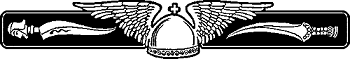
\includegraphics[width=9.3cm]{viking-tales/028}\\
    The Sea Fight}

\lettrine{M}{any} men felt as Solfi did. So when King Audbiorn and King
Arnvid sent out their war arrows, a great host gathered. All men came by
sea. Two hundred ships lay at anchor in the fiord, looking like strange
swimming animals because of their high carved prows and bright paint.
There were red and gold dragons with long necks and curved tails.
Sea-horses reared out of the water. Green and gold snakes coiled up.
Sea-hawks sat with spread wings ready to fly. And among all these curved
necks stood up the tall, straight masts with the long yardarms swinging
across them holding the looped-up sails.

When the starting horn blew, and their sails were let down, it was like
the spreading of hundreds of curious flags. Some were striped black and
yellow or blue and gold. Some were white with a black raven or a brown
bear embroidered on them, or blue with a white sea-hawk, or black with a
gold sun. Some were edged with fur. As the wind filled the gaudy sails,
and the ships moved off, the men waved their hands to the women on shore
and sang:

\begin{quote}
``To the sea! To the sea!\\
The wind in our sail,\\
The sea in our face,\\
And the smell of the fight.\\
After ship meets ship,\\
In the quarrel of swords\\
King Harald shall lie\\
In the caves under sea\\
And Norsemen shall laugh.''
\end{quote}

In the prow stood men leaning forward and sniffing the salt air with
joy. Some were talking of King Harald.

``Yesterday he had a hard fight,'' they said. ``To-day he will be lying
still, dressing his wounds and mending his ships. We shall take him by
surprise.''

They sailed near the coast. Solfi in his ``Sea-hawk'' was ahead leading
the way. Suddenly men saw his sail veer and his oars flash out. He had
quickly turned his boat and was rowing back. He came close to King
Arnvid and called:

``He is there, ahead. His boats are ready in line of battle. The fox has
not been asleep.''

King Arnvid blew his horn. Slowly his boats came into line with his
``Sea-stag'' in the middle. Again he blew his horn. Cables were thrown
across from one prow to the next, and all the ships were tied together
so that their sides touched. Then the men set their sails again and they
went past a tongue of land into a broad fiord. There lay the long line
of King Harald's ships with their fierce heads grinning and mocking at
the newcomers. Back of those prows was what looked like a long wall with
spots of green and red and blue and yellow and shining gold. It was the
locked shields of the men in the bows, and over every shield looked
fierce blue eyes. Higher up and farther back was another wall of
shields; for on the half deck in the stern of every ship stood the
captain with his shield-guard of a dozen men.

Arnvid's people had furled their sails and were taking down the masts,
but the ships were still drifting on with the wind. The horn blew, and
quickly every man sprang to his place in bow and stern. All were leaning
forward with clenched teeth and widespread nostrils. They were clutching
their naked swords in their hands. Their flashing eyes looked over their
shields.

Soon King Arnvid's ships crashed into Harald's line, and immediately the
men in the bows began to swing their swords at one another. The soldiers
of the shield-guard on the high decks began to throw darts and stones
and to shoot arrows into the ships opposite them.

So in every ship showers of stones and arrows were falling, and many men
died under them or got broken arms or legs. Spears were hurled from deck
to deck and many of them bit deep into men's bodies. In every bow men
slashed with their swords at the foes in the opposite ship. Some jumped
upon the gunwale to get nearer or hung from the prow-head. Some even
leaped into the enemy's boat.

King Harald's ship lay prow to prow with King Arnvid's. The battle had
been going on for an hour. King Harald was still in the stern on the
deck. There was a dent in his helmet where a great stone had struck.
There was a gash in his shoulder where a spear had cut. But he was still
fighting and laughed as he worked.

``Wolf meets wolf to-day,'' he said. ``But things are going badly in the
prow,'' he cried. ``Ivar fallen, Thorstein wounded, a dozen men lying in
the bottom of the boat!''

He leaped down from the deck and ran along the gunwale, shouting as he
went:

``Harald and victory!''

So he came to the bow and stood swinging his sword as fast as he
breathed. Every time it hit a man of Arnvid's men. Harald's own warriors
cheered, seeing him.

``Harald and victory!'' they shouted, and went to work again with good
heart.

Slowly King Arnvid's men fell back before Harald's biting sword. Then
Harald's men threw a great hook into that boat and pulled it alongside
and still pushed King Arnvid's people back.

``Come on! Follow me!'' cried Harald.

Then he leaped into King Arnvid's boat, and his warriors followed him.

``He comes like a mad wolf,'' King Arnvid's men said, and they turned
and ran back below the deck.

Then Arnvid himself leaped down and stood with his sword raised.

``Can this young Shockhead make cowards of you all?'' he cried.

But Harald's sword struck him, and he fell dead. Then a big, bloody
viking of King Arnvid leaped upon the edge of the ship and stood there.
He held his drinking-horn and his sword high in his hands.

``Ran\footnote{See note about Ran on page~\pageref{ran}.} and not you,
Shockhead, shall have them and me!'' he cried, and leaped laughing into
the water and was drowned.

Many other warriors chose the same death on that terrible day.

\begin{figure}[ht]
    \centering
    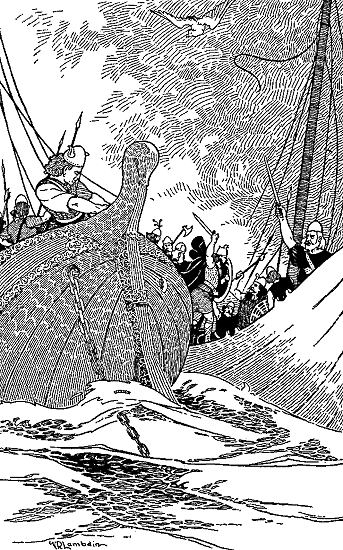
\includegraphics[width=9.1cm]{viking-tales/029}
    \caption{``Then he leaped into King Arnvid's boat''}
\end{figure}

All along the line of boats men fought for hours. In some places the
cables had been cut, and the boats had drifted apart. Ships lay
scattered about two by two, fighting. May boats sank, many men died,
some fled away in their ships, and at the end King Harald had won the
battle. So he had King Arnvid's country and King Audbiorn's country.
Many men took the oath and became his friends. All people were talking
of his wonderful battles.

\begin{figure}[hb]
    \centering
    \vskip8pt
    
\includegraphics[width=2.7cm]{viking-tales/017}
\end{figure}

    \section[King Harald's Wedding]{
    
\includegraphics[width=9.3cm]{viking-tales/030}\\
    King Harald's Wedding}

\lettrine{I}{t} had taken King Harald ten years to fight so many battles.
And all that time he had not cut his hair or combed it. Now he was
feasting one day at an earl's house. Many people were there.

``How is it, friends?'' Harald said. ``Have I kept my vow?''

His friends answered:

``You have kept your vow. There is no king but you in all Norway.''

``Then I think I will cut my hair,'' the king laughed.

So he went and bathed and put on fresh clothes. Then the earl cut his
hair and beard and combed them and put a gold band about his head. Then
he looked at him and said:

``It is beautiful, smooth, and yellow.''

And all people wondered at the beauty of the king's hair.

``I will give you a new name,'' the earl said. ``You shall no longer be
called Shockhead. You shall be called Harald Hairfair.''

``It is a good name,'' everybody cried.

Then Harald said:

``But I have another thing to do now. Guthorm, you shall take the same
message to Gyda that you gave ten years ago.''

So Guthorm went and brought back this answer from Gyda:

``I will marry the king of all Norway.''

So when the wedding time came, Harald rode across the country to the
home of Gyda's father, Eric. Many men followed him. They were all richly
dressed in velvet and gold.

For three nights they feasted at Eric's house. On the next night Gyda
sat on the cross-bench with her women. A long veil of white linen
covered her face and head and hung down to the ground. After the
mead-horns had been brought in, Eric stood up from his high seat and
went down and stood before King Harald.

``Will you marry Gyda now?'' he asked.

\begin{figure}
    \centering
    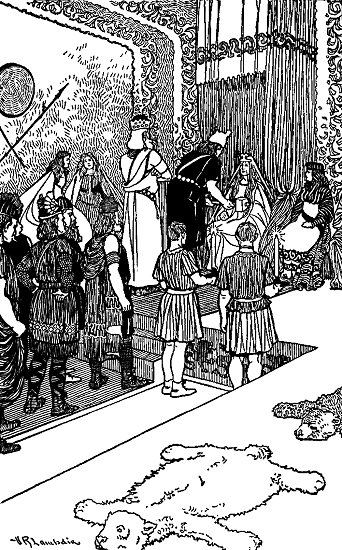
\includegraphics[width=9.1cm]{viking-tales/031}
    \caption{``I, Harald, King of Norway, take you Gyda, for my wife''}
\end{figure}

Harald jumped to his feet and laughed.

``Yes,'' he said. ``I have waited long enough.''

Then he stepped down from his high seat and stood by Eric. They walked
about the hall. Before them walked thralls carrying candles. Behind them
walked many of King Harald's great earls. Three times they walked around
the hall. The third time they stopped before the cross-bench. King
Harald and Eric stepped upon the platform, where the cross-bench was.

Eric gave a holy hammer to Harald, and it was like the hammer of Thor.
Harald put it upon Gyda's lap, saying:

``With this holy hammer of Thor's, I, Harald, King of Norway, take you,
Gyda, for my wife.''

Then he took a bunch of keys and tied it to Gyda's girdle, saying:

``This is the sign that you are mistress of my house.''

After that, Eric called out loudly:

``Now, are Harald, King of Norway, and Gyda, daughter of Eric, man and
wife.''

Then thralls brought meat and drink in golden dishes. They were about to
serve it to Gyda for the bride's feast, but Harald took the dish from
them and said:

``No, I will serve my bride.''

So he knelt and held the platter. When he did that his men shouted. Then
they talked among themselves, saying:

``Surely Harald never knelt before. It is always other people who kneel
to him.''

When the bride had tasted the food and touched the mead-horn to her lips
she stood up and walked from the hall. All her women followed her, but
the men stayed and feasted long.

On the next morning at breakfast Gyda sat by Harald's side. Soon the
king rose and said:

``Father-in-law, our horses stand ready in the yard. Work is waiting for
me at home and on the sea. Lead out the bride.''

So Eric took Gyda by the hand and led her out of the hall. Harald
followed close. When they passed through the door Eric said:

``With this hand I lead my daughter out of my house and give her to you,
Harald, son of Halfdan, to be your wife. May all the gods make you
happy!''

Harald led his bride to the horse and lifted her up and set her behind
his saddle and said:

``Now this Gyda is my wife.''

Then they drank the stirrup-horn and rode off.

``Everything comes to King Harald,'' his men said; ``wife and land and
crown and victory in battle. He is a lucky man.''

\begin{figure}[hb]
    \centering
    \vskip8pt
    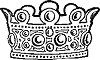
\includegraphics[width=2.7cm]{viking-tales/014}
\end{figure}

    \chapter[King Harald Goes West-Over-Seas]{
    
\includegraphics[width=9.3cm]{viking-tales/032}\\
    King Harald Goes West-Over-Seas}

\lettrine{N}{ow} many men hated King Harald. Many a man said:
\vskip2\baselineskip
``Why should he put himself up for king of all of us? He is no better
than I am. Am I not a king's son as well as he? And are not many of us
kings' sons? I will not kneel before him and promise to be his man. I
will not pay him taxes. I will not have his earl sitting over me. The
good old days have gone. This Norway has become a prison. I will go away
and find some other place.''

So hundreds of men sailed away. Some went to France and got land and
lived there. Big Rolf-go-afoot and all his men sailed up the great
French River and won a battle against the French king himself. There was
no way to stop the flashing of his battle-axes but to give him what he
wanted. So the king made Rolf a duke, gave him broad lands and gave him
the king's own daughter for wife. Rolf called his country Normandy, for
old Norway. He ruled it well and was a great lord, and his sons' sons
after him were kings of England.

Other Norsemen went to Ireland and England and Scotland. They drew up
their boats on the river banks. The people ran away before them and
gathered into great armies that marched back to meet the vikings in
battle. Sometimes the Norsemen lost, but oftener they won, so that they
got land and lived in those countries. Their houses sat in these strange
lands like warriors' camps, and the Norsemen went among their new
neighbors with hanging swords and spears in hand, ever ready for fight.

There are many islands north of Scotland. They are called the Orkneys
and the Shetlands. They have many good harbors for ships. They are
little and rocky and bare of trees. Wild sea-birds scream around them.
On some of them a man can stand in the middle and see the ocean all
about him. Now the vikings sailed to these islands and were pleased.

\begin{figure}
    \centering
    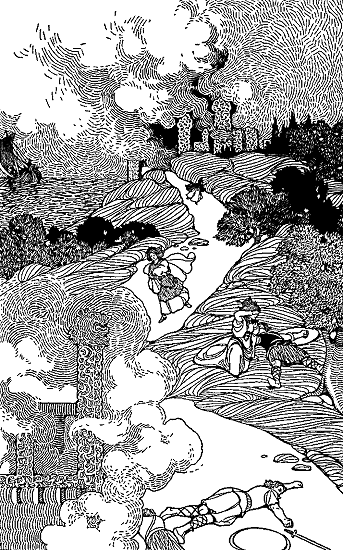
\includegraphics[width=9.1cm]{viking-tales/033}
    \caption{``In Norway they left burning houses and weeping women''}
\end{figure}

``It is like being always in a boat,'' they said. ``This shall be our
home.''

So it went until all the lands round about were covered with vikings.
Norse carved and painted houses brightened the hillsides. Viking ships
sailed all the seas and made harbor in every river. Norsemen's thralls
plowed the soil and planted crops and herded cattle, and gold flowed
into their masters' treasure-chests. Norse warriors walked up and down
the land, and no man dared to say them nay.

These men did not forget Norway. In the summers they sailed back there
and harried the coast. They took gold and grain and beautiful cloth back
to their homes. In Norway they left burning houses and weeping women.

Every summer King Harald had out his ships and men and hunted these
vikings. There are many little islands about Norway. They have crags and
caves and deep woods. Here the vikings hid when they saw King Harald's
ships coming. But Harald ran his boat into every creek and fiord and
hunted in every cave and through all the woods and among the crags. He
caught many men, but most of them got away and went home laughing at
Harald. Then they came back the next summer and did the same deeds over
again. At last King Harald said:

``There is but one thing to do. I must sail to these western islands and
whip these robbers in their own homes.''

So he went with a great number of ships. He found as brave men as he had
brought from Norway. These vikings had brought their old courage to
their new homes. King Harald's fine ships were scarred by viking stones
and scorched by viking fire. The shields of Harald's warriors had dents
from viking blows. Many of those men carried viking scars all their
lives. And many of King Harald's warriors walked the long, hard road to
Valhalla, and feasted there with some of these very vikings that had
died in King Harald's battles. But after many hard fights on land and
sea, after many men had died and many had fled away to other lands, King
Harald won, and he made the men that were yet in the islands take the
oath, and he left his earls to rule over them. Then he went back to
Norway.

``He has done more than he vowed to do,'' people said. ``He has not only
whipped the vikings, but he has got a new kingdom west-over-seas.''

Then they talked of that dream that his mother had.

``King Harald was that great tree,'' they said. ``The trunk was red with
the blood of his many battles, but higher up the limbs were fair and
green like this good time of peace. The topmost branches were white
because Harald will live to be an old man. Just as that tree spread out
until all of Norway was in its shade, and even more lands, so Harald is
king of all this country and of the western islands. The many branches
of that tree are the many sons of Harald, who shall be earls and kings
in Norway, and their sons after them, for hundreds of years.''


    \cleardoublepage
    \part[West-Over-Seas]{
        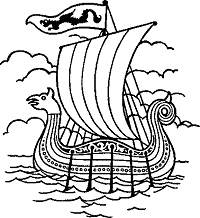
\includegraphics[width=5.3cm]{viking-tales/034}\\[1cm]
        West-Over-Seas
        \partfig}
    \section[Homes in Iceland]{
    
\includegraphics[width=9.3cm]{viking-tales/035}\\
    Homes in Iceland}

\lettrine{M}{en} had been feasting in Ingolf's house. But there was no
laughing and no shouting of jokes. Ingolf sat in his high seat frowning
and gloomy. His head hung on his breast. He was staring into the fire.
Now he raised his head and looked about the hall.

``Comrades,'' he said, ``what shall we do? Herstein and Holmstein died
by our swords. Their kinsmen hunger to kill us. Besides, when Harald
hears of our deed, there will not be a safe place in Norway for us. He
will never let a man fight out an honest quarrel. Where shall we go?''

A man stood up from the bench.

``We have friends in the Shetlands,'' he said. ``Let us find homes
there.''

Then Leif, in the high seat opposite Ingolf, stood up.

``No, not the Shetlands, my foster-brother.\footnote{See note about
foster-brothers on page~\pageref{foster-brothers}.} They are crowded
already. Besides, Harald will not long keep his hands off them. Then they
will be no better than Norway. England and Ireland and Scotland are old.
My eyes ache for something new. What of that far island that Floki found?
It is empty. We could choose our land from the whole country. There is
good fishing. There are green valleys. And Butter Thorolf says that
butter drops from every weed. There are mountains and deserts where we
may find adventure. I say, let us steer for Iceland!''

When he stopped, many of the men shouted:

``Yes! Iceland!''

But an old man stood up.

``We have all laughed at that tale of Butter Thorolf's,'' he said. ``But
Floki himself said that the sea about the island is full of ice that
pushes upon the land, that no ship can live in that water in the winter,
that great mountains of ice cover the island. Did not all his cattle die
there of hunger and cold, and did he not come back to Norway cursing
Iceland?''

``Oh, Sighvat, you are old and fearful,'' called out Leif, and he
laughed.

Then he stretched himself up and threw back his head.

``Are we afraid of ice? Have we not seen angry water before? I have been
hungry, but I have never died of it. Surely if there are fish in the sea
and grass in the valleys, we can live there. I should like to stand on a
hill and look around on a wide land and think, `This is all ours,' and
out upon a rough sea and think, `Far off there are our foes and they
dare not come over to us.' Besides, we shall have no Shockhead Harald to
lord it over us. We can come and go and feast and fight as we please. We
shall be our own kings. And our ships will be always waiting to take us
away, when we are weary of it. And we shall see things that other men
have never seen. I am tired of the old things. Perhaps in after days men
will make songs about `those foster-brothers, Ingolf and Leif, who made
a new country in a wonderful land, and whose sons and grandsons are
mighty men in Iceland!'''

Ingolf leaped up from his chair.

``By the strong arm of Thor!'' he cried, ``I like the sound of it. Now I
make my vow.''

He raised his drinking-horn.

``I vow that I will find this Iceland and pass the winter there, and
that if man can live upon it I will go back there and set up my home.''

``And I vow that I will follow my foster-brother,'' cried Leif.

And many men vowed to go.

So on the next day they began to make ready a boat. They looked her over
carefully and recalked every seam and freshly painted her and put into
her their strongest oars and made her a new sail.

``This will be the longest voyage that she ever made,'' Ingolf said.

When the work was done, they put into her great stores, axes, hammers,
fish-nets, cooking-kettles, kegs of ale, chests of hard bread, chests of
smoked meat, brass kettles full of flour, skin bottles of water. They
stowed these things away in the ends of the ship. When they were ready
they put in four head of cattle.

``We shall need the milk and perhaps the meat,'' Ingolf said.

Many men wished to go, but Ingolf had said:

``There is little room to spare and little food and drink. I have
planned for half a year. But perhaps we must be sailing longer than
that. Our food may run short. We must not have extra mouths to feed.
There are thirty oars in our boat. I will take only one man for every
oar, and Leif and I will steer.''

So they started off. Leif stood in the prow leaning forward and looking
far ahead, and he sang:

\begin{quote}
``What does the swimming dragon smell?\\
A stormy sea, an empty land,\\
Hunger, darkness, giants, fire.\\
Leif and his sword do laugh at that.''
\end{quote}

They sailed for days and saw no land. Sometimes they passed ships and
always made sure to sail close enough to hail them.

``Where are you going?'' Ingolf would call.

``To Norway,'' would come back the answer.

``For trade or fight?'' Leif would shout.

Then would ring out a great laugh from that boat and this answer:

``A shut mouth is a good friend.''

So the two ships sailed on, and the men were glad to have heard a
greeting and to have called one.

But at last there were the Shetlands.

``We will go in here and rest,'' Ingolf said.

When they rowed to shore a certain Shetland man stood there. He watched
them land and looked them all over. Then he walked up to Ingolf and
said:

``You look like brave men. Welcome to Shetland. You shall come to my
house and rest your legs from ship-going and fill your stomachs. I
hunger for news of Norway.''

So they went to his house and stayed there for three days. And good it
seemed to be near a fire and in a quiet bed and before a steaming
platter. When they went to the shore to start off again, the Shetland
man had his thralls carry a keg of ale and a great kettle of cooked meat
and put them into the ship.

``Think of me when you eat this,'' he said.

Then the Norsemen put to sea again and sailed for a long time.

One day a terrible storm came up; the sky was black; the wind howled
through the ship. Great waves leaped in the sea.

``Down with the sail and out with the oars!'' Ingolf shouted.

So the men furled the sail and took down the mast and laid it along the
bottom of the boat. As they worked, one man was washed overboard and
drowned. The men sat down to row, but the tumbling waves tossed the boat
about and poured over her and broke three of the oars. But still the men
held on. They were wet to the skin and were cold, and their arms and
legs ached with the hard work, and they were hungry from the long
waiting, but not one face was white with fear.

``Ran, in her caves under sea, wants us for company to-night,'' Ingolf
laughed.

So they tossed about all night, but in the morning the wind died down.
Great waves still rolled, and for days the sea was rough, but they could
put up the sail. Then one day Leif, as he sat in the pilot's seat,
jumped to his feet and sang:

\begin{quote}
``To eyes grown tired with looking far,\\
All at once appeared an island,\\
A stretching-place for sea-legs,\\
A quiet bed for backs grown stiff\\
On rowing-bench on rolling sea.\\
A place to build a red fire\\
And thaw the blood that sea-winds froze.''
\end{quote}

But when they came near they saw no place to land. The island was like a
mountain of rock standing out of the water. The sides were steep and
smooth. They sailed around it, but found no place to climb up.

``There are many other islands here,'' said Leif. ``We will try
another.''

So he steered to another. It, too, was a steep rock, but one side sloped
down to the water and was green with grass.

``Oh, I have not seen anything so good as that green grass since I
looked into my mother's face,'' one man said.

There was a little harbor there. The men rowed in and quickly jumped out
and put the rollers under the ship and pulled her upon shore. Then they
threw themselves down on the grass and rolled and stretched their arms
and shouted for joy. After that they built a fire and warmed themselves
and cooked a meal and ate like wolves. They slept there that night.

In the morning before Ingolf's men started away they were standing high
up on the hillside, looking about. They saw no houses on any of the
islands, but they saw smoke rise from one hillside.

``Some other men, like us, weary of the sea and stopping to rest,'' said
Ingolf.

They saw the island that they had sailed around the night before.

``There can surely be nothing but birds' nests on top of that,'' Sighvat
said.

``Look!'' cried another, pointing.

Men were standing on the flat top of that island. They were letting a
boat down the steep side with ropes. When it struck the water, they made
a rope fast to the rock and slid down it into the ship and sailed off.

``Some robber vikings from Scotland or Ireland,'' laughed Leif. ``It is
a good hiding place for treasure.''

Soon Ingolf and his men got into their ship and were off. Old Sighvat
grumbled.

``Is this land not new enough and empty enough and far enough? I am
tired of sea, sea, sea, and nothing else.''

``We started for Iceland,'' said Ingolf, ``and I will not stop before I
come there. I have a vow. Did you make none, Sighvat?''

Then they were on the water again for weeks with no sight of land.

``Oh! I would give my right hand to see a dragon pawing the water off
there and to fling a word to its men,'' Sighvat said.

``No hope of that,'' replied Ingolf. ``Only three dragons before ours
have ever swept this water, and men are not sailing this way for
pleasure or riches.''

So only the desolate sea stretched around them. Sometimes it was smooth
and shining under the sun. Often it was torn by winds, and a gray sky
hung over it, and the men were drenched with rain. Once they ran into a
fog. For three days and nights they could not see sun or stars to steer
by. They forgot which way was north. When after three days the fog
lifted, they found that they had been going in the wrong direction, and
they had to turn around and sail all that weary way over again. But at
last one afternoon they saw a white cloud resting on the water far off.
As they sailed toward it, it grew into long stretches of black, hilly
shore with a blue ice mountain rising from it. The sun was going down
behind that mountain, and long lines of pink and of shining green, and
great purple shadows streaked the blue.

``It is Iceland!'' shouted the men.

``It is like Asgard the Shining,'' Ingolf said.

But it was still far off. Men can see a long way there because the air
is so clear. So Ingolf and his people sailed on for hours and at last
came into a harbor. A little green valley sloped up from it. On one side
was the bright ice mountain. Back of it were bare black and red hills.
In that valley Ingolf and his men drew up their boat and camped. At
supper that night one of the men said:

``I almost think I never felt a fire before or had warm food in my
mouth.''

The men laughed.

``It is four months since we left Norway,'' Ingolf said. ``Few men have
ever been on the sea so long.''

That night they put up the awning in the boat and slept under it.

After that some men went fishing every day in the rowboat that they had.
And Ingolf took others, and they sailed along the shore, seeing what
kind of a land this was. But winter began to come on. Then Ingolf said:

``Remember what Floki said of the ice and the rough sea in winter. Soon
we cannot sail any longer. Let us choose a place to stay and build a hut
there and cut hay for our cattle.''

So they did. Their hut was a little mean thing of stones and turf. They
kept the cattle and the hay in it. Sometimes they slept there, when it
was very cold. But most of the time they ate and slept by a great
bonfire out of doors where it was clean. Leif said:

``I like the cold air of the sea better than the bad-smelling air of a
house, even though it is warm.''

Now every day Ingolf and Leif and some of the men walked about the
island. At night they all sat around the campfire and talked of what
they had seen during the day.

``This is surely a wonderful land,'' Ingolf said once. ``It is at the
same time like Niflheim and like Asgard. Here is a spot green and soft,
a sweet cradle for men. Next it is a mountain of ice where men would
freeze to death. And next to that is a hill of rock that seems to have
come out of some great fire. Yesterday I saw a cave on the seashore. The
door of it was big enough for a giant. The waves broke at the doorstep.
A terrible roaring came from the cave. I think it is the home of a
giant. I think that giants of fire and giants of frost made this island.
I have seen great basins in the rocks filled with warm water. They
looked like giants' bath-tubs. I have seen boiling water shoot up out of
the ground. I have walked, and have felt and heard a great rumbling
under me as though some giant were sleeping there and turning over in
his sleep. One day I stood on a mountain and looked inland. There was a
wide desert of sand and black and red rock with nothing growing on it.
The fierce wind blew dirt into my eyes, and the cold of it froze the
marrow in my bones. When I have seen these things I have cursed the
country, and have said: `The gods hate Iceland. I will not stay here.'
But then I have walked through beautiful warm valleys where the winds
did not come. I saw in my mind the flowers that we found last summer. I
saw our cattle feeding on the sweet grass. I thought of the sea full of
good fish. I saw my house built among green fields, and my wife sitting
in her home, and my children playing among the flowers and making up
tales about the bright ice mountains. I saw the wide, rough seas between
me and Harald and our foes. Then I thought to myself, `It is the
sweetest home on earth.' As for me, I am coming here to live. What do
you say, comrades?''

``Have I not vowed to follow you, foster-brother?'' said Leif. ``And
indeed I never saw a land that I liked better. I don't believe in your
giants. My sword is my god, and my ship is my temple, and I like this
land to set them up in.''

They sat about the fire long that night making plans.

``You shall go home and get our women and our things, Ingolf,'' said
Leif. ``I will off to Ireland and have a frolic. There will be little
play of swords in this empty land, and I want to have one last game
before I hang up my battle-knife. Besides, I will come to you with a
ship full of gold and clothes and house-hangings such as we cannot get
here, and they will cost me nothing but the swing of a sword.''

As they talked, Ingolf looked up at the sky. The northern lights were
quivering there. They were like great flames of yellow and green and
red.

``See,'' he said, and pointed. ``We are not so far that the gods will
forget us. There is the flash of the armor of the Valkyrias.\footnote{See
note about Valkyrias on page~\pageref{valkyrias}.} A battle is on
somewhere, and Odin has sent his maidens to choose the heroes for
Valhalla.''

Leif only laughed and lay down to sleep.

So in the spring they all went back to Norway. Leif got ready the boat
again and merrily sailed for Ireland.

``Here I go to get riches for our new land,'' he said.

Ingolf set his men to cutting down pines in the forest and some to
building a new ship. He had his thralls plant large crops of grain and
grind flour and make new kegs and chests of wood. He himself worked much
at the forge, making all kinds of tools--spades, axes, hammers,
hunting-knives, cooking kettles. The women were busy weaving and sewing
new clothes. Ingolf sold his house and land and everything that he could
not take with him.

After about two years Leif came back. He had ten thralls that he had got
in Ireland. He took Ingolf aboard his ship and raised the covers of
great chests. Gold helmets, silver-trimmed drinking-horns, embroidered
robes, and swords flashed out.

``Did I not say that I would come back with a full ship?'' he laughed.

At last all things were ready for starting.

``To-day I will sacrifice to Thor and Odin,'' Ingolf said. ``If the
omens are good we will start to-morrow.''

``Well, go, foster-brother,'' laughed Leif. ``But I have better things
to do. I will be putting the cattle into the ship and will have all
ready.''

So Ingolf and his men went into the forests a little way. There in a
cleared space stood a large building. In front of this temple the men
killed two horses for Odin. Ingolf caught some of the blood in a brass
bowl. He raised it and looked up at the sky and said:

``All-wise and all-father Odin, and Thor who loves the thunder, I give
these horses to you. Tell me whether it is your will that we go to
Iceland.''

As he said that, a raven flew over his head. Ingolf watched it.

``It is Odin's will that we go,'' he said. ``He sent his raven\footnote{
See note about Odin's ravens on page~\pageref{odins-ravens}.} to tell us.
It is flying straight toward Iceland.''

The men shouted with joy at that.

Now they hung some of the meat of the horses on a tree near the temple.

``For the ravens of Odin,'' they said.

Ingolf carried the bowl of blood into the temple. He went through the
feast hall in front to a little room at the back. Here stood wooden
statues of the gods in a semicircle. Before them was a stone altar.
Ingolf took a little brush of twigs that lay on it and dipped it into
the blood and sprinkled the statues.

``You shall taste of our sacrifice,'' he said. ``Look kindly on us from
your happy seats in Asgard.''

Then they went into the feast hall. There thralls were boiling the
horseflesh in pots over the fire. The tables were standing ready before
the benches. Ingolf walked to the high seat. All the others took their
places at the benches. When the horns came round, Ingolf made this vow:

``I vow that I will build my house wherever these pillars lead me.''

He put his hand upon a tall post that stood beside the high seat. There
was one at each side. They were the front posts of the chair. But they
stood up high, almost to the roof. They were wonderfully carved and
painted with men and dragons. On the top of each one was a little statue
of Thor with his hammer.

At the end of the feast Ingolf had his thralls dig these pillars up. He
had a little bronze chest filled with the earth that was under the
altar.

``I will take the pillars of my high seat to Iceland,'' he said, ``and I
will set up my altar there upon the soil of Norway, the soil that all my
ancestors have trod, the soil that Thor loves.''

So they carried the pillars and the chest of earth and the statues of
the gods, and put them into Ingolf's boat.

``It is a well-packed ship,'' the men said. ``There is no spot to
spare.''

Tools, and chests of food, and tubs of drink, and chests of clothes, and
fishing nets were stowed in the bows of both boats. In the bottom were
laid some long, heavy, hewn logs.

``The trees in Iceland are little,'' Ingolf said. ``We must take the
great beams for our homes with us.''

Standing on these logs were a few cattle and sheep and horses and pigs.
The rowers' benches were along the sides. In the stern of each boat was
a little cabin. Here the women and children were to sleep. But the men
would sleep on the timbers in the middle of the boat and perhaps they
would put up the awning sometimes.

At last everyone was aboard. Men loosed the rope that held the boats.
The ships flashed down the rollers into the water, and Ingolf and Leif
were off for Iceland. As they sailed away everyone looked back at the
shore of old Norway. There were tears in the women's eyes. Helga, Leif's
wife, sang:

\begin{quote}
``There was I born. There was I wed.\\
There are my father's bones.\\
There are the hills and fields,\\
The streams and rocks that I love.\\
There are houses and temples,\\
Women and warriors and feasts,\\
Ships and songs and fights--\\
A crowded, joyous land.\\
I go to an empty land.''
\end{quote}

There was the same long voyage with storm and fog. But at last the
people saw again the white cloud and saw it growing into land and
mountains. Then Ingolf took the pillars of his high seat and threw them
overboard.

``Guide them to a good place, O Thor!'' he cried.

The waves caught them up and rolled them about. Ingolf followed them
with his ship. But soon a storm came up. The men had to take down the
sails and masts, and they could do nothing with their oars. The two
ships tossed about in the sea wherever the waves sent them. The pillars
drifted away, and Ingolf could not see them.

``Remember your pillars, O Thor!'' he cried.

Then he saw that Leif's ship was being driven far off.

``Ah, my foster-brother,'' he thought, ``shall I not have you to cheer
me in this empty land? O Thor, let him not go down to the caves of Ran!
He is too good a man for that.''

On the next day the storm was not so hard, and Ingolf put in at a good
harbor. A high rocky point stuck out into the sea. A broad bay with
islands in the mouth was at the side. Behind the rocky point was a level
green place with ice-mountains shining far back.

After a day or two Ingolf said:

``I will go look for my pillars.''

So he and a few men got into the rowboat and went along the shore and
into all the fiords, but they could not find the pillars. After a week
they came back, and Ingolf said:

``I will build a house here to live in while I look for the posts. This
way is uncomfortable for the women.''

So he did. Then he set out again to look for the pillars, but he had no
better luck and came back.

``I must stay at home and see to the making of hay and the drying of
fish,'' he said. ``Winter is coming on, and we must not be caught with
nothing to eat.''

So he stayed and worked and sent two of his thralls to look for the holy
posts. They came back every week or two and always had to say that they
had not found them. Midwinter was coming on.

\begin{figure}
    \centering
    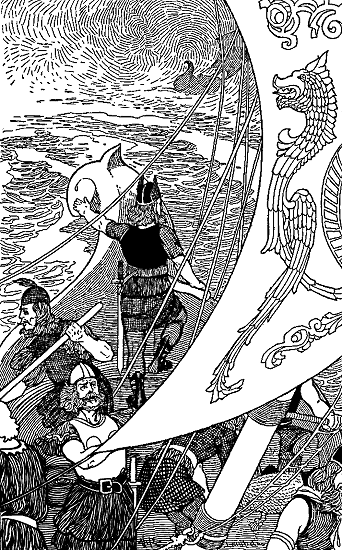
\includegraphics[width=9.1cm]{viking-tales/036}
    \caption{``Then he saw that Leif's ship was being driven afar off''}
\end{figure}

``Ah!'' said Ingolf's wife one day, ``do you remember the gay feast that
we had at Yule-time? All our friends were there. The house rang with
song and laughter. Our tables bent with good things to eat. Walls were
hung with gay draperies. The floor was clean with sweet-smelling
pine-branches. Now look at this mean house; its dirt floor, its bare
stone walls, its littleness, its darkness! Look at our long faces. No
one here could make a song if he tried. Oh! I am sick for dear old
Norway.''

``It is Thor's fault,'' Ingolf cried. ``He will not let me find his
posts.''

He strode out of the house and stood scowling at the gray sea.

``Ah, foster-brother!'' he said. ``It was never so gloomy when you were
by my side. Where are you now? Shall I never hear your merry laugh
again? That spot in my palm burns, and my heart aches to see you. That
arch of sod keeps rising before my eyes. Our vows keep ringing in my
ears.''

At last the long, gloomy winter passed and spring came.

``Cheer up, good wife,'' Ingolf said. ``Better days are coming now.''

But that same day the thralls came back from looking for the posts.

``We have bad news,'' they said. ``As we walked along the shore looking
for the pillars we saw a man lying on the shore. We went up to him. He
was dead. It was Leif. Two well-built houses stood near. We went to
them. We knew from the carving on the door-posts that they were Leif's.
We went in. The rooms were empty. Along the shore and in the wood back
of the house we found all of his men, dead. There was no living thing
about.''

Ingolf said no word, but his face was white, and his mouth was set. He
went into the house and got his spears and his shield and said to his
men:

``Follow me.''

They put provisions into the boat and pushed off and sailed until they
saw Leif's houses on the shore of the harbor. There they saw Leif and
the men who were his friends, dead. Their swords and spears were gone.
Ingolf walked through the houses calling on Helga and on the thralls,
but no one answered. The storehouse was empty. The rich hangings were
gone from the walls of the houses. There was nothing in the stables. The
boat was gone.

Ingolf went out and stood on a high point of land that jutted out into
the water. Far along the coast he saw some little islands. He turned to
his men and said:

``The thralls have done it. I think we shall find them on those
islands.''

Then he went back to Leif and stood looking at him.

``What a shame for so brave a man to fall by the hands of thralls! But I
have found that such things always happen to men who do not sacrifice to
the gods. Ah, Leif! I did not think when we made those vows of
foster-brotherhood that this would ever happen. But do not fear. I
remember my promise. I had thought that a man's blood is precious in
this empty land, but my vow is more precious.''

Now they laid all those men together and tied on their hell-shoes.

``I need my sword for your sake, foster-brother. I cannot give you that.
But you shall have my spears and my drinking-horn,'' said Ingolf. ``For
surely Odin has chosen you for Valhalla, even though you did not
sacrifice. You are too good a man to go to Niflheim. You would make
times merry in Valhalla.''

So Ingolf put his spears and his drinking-horn by Leif. Then the men
raised a great mound over all the dead. After that they went aboard
their boat and sailed for the islands that Ingolf had seen. It was
evening when they reached them.

``I see smoke rising from that one,'' Ingolf said, pointing.

He steered for it. It was a steep rock like that one in the Faroes, but
they found a harbor and landed and climbed the steep hill and came out
on top. They saw the ten thralls sitting about a bonfire eating. Helga
and the other women from Leif's house sat near, huddled together, white
and frightened. One of the thralls gave a great laugh and shouted:

``This is better than pulling Leif's plow. To-morrow we will sail for
Ireland with all his wealth.''

``To-morrow you will be freezing in Niflheim,'' cried Ingolf, and he
leaped among them swinging his sword, and all his men followed him, and
they killed those thralls.

Then Ingolf turned to Helga. She threw herself into his arms and wept.
But after a while she told him this story:

``When springtime came, Leif thought that he would sow wheat. He had but
one ox. The others had died during the winter. So he set the thralls to
help pull the plow. I saw their sour looks and was afraid, but Leif only
laughed:

```What else can thralls expect?' he said. `Never fear them, good wife.'

``Now one day soon after that the thralls came running to the house
calling out:

```The ox is dead! The ox is dead!'

``Leif asked them about it. They said that a bear had come out of the
woods and killed it, and that they had scared the beast away. They
pointed out where it had gone. Then Leif called his men and said:

```A hunt! I had not hoped for such great sport here. Ah, we will have a
feast off that bear!'

``So they took their spears and went out into the woods. As soon as they
were gone, the thralls came running into the house and took down all the
swords and shields from the wall and ran out. In some way they met my
lord and his men in the woods and killed them. Then they came back and
took everything in the house and dragged us to the boat and sailed
here.''

``O my brother!'' said Ingolf, ``where is that song about `those two
foster-brothers, Ingolf and Leif, who made a new country in a wonderful
land, and whose sons and grandsons are mighty men in Iceland'? But come
home with me, Helga.''

So they took the women and Leif's things and Leif's boat and sailed
home. The next day after they came to Ingolf's house, Helga said:

``We have made your family larger, brother Ingolf. Will you not take
Leif's two houses and live in them? He does not need them now. He would
like you to have them.''

``It would be pleasant to live there,'' Ingolf said. ``I thank you.''

So the next day they loaded everything aboard the two ships and sailed
for Leif's house. There they stayed for a year. Ingolf still sent his
thralls out to look for the pillars. He was careful always to have hay,
so his cattle prospered. That spring he planted wheat, but it did not
grow well.

``This is sickly stuff,'' Ingolf said. ``It takes too much time and
work. It is better to save the land for hay. Perhaps we can sometime go
back to Norway for flour.''

At last one day the thralls came home and said:

``We have found the pillars.''

Ingolf jumped to his feet. He cried out:

``You have kept me waiting three years, Thor. But as soon as my house
and temple are built, I will sacrifice to you three horses as a
thank-offering.''

``It is a long way off, master,'' the thralls said, ``and we have found
much better places in our walks about the island.''

``Thor knows best,'' Ingolf answered. ``I will settle where he leads
me.''

So that summer they loaded everything into the ships again and sailed
west along the coast until they came to the place where the pillars
were. The land there was low and green. On both sides were low hills. A
little lake glistened back from shore. In the valley were hot springs,
with steam rising from them.

``It looks like smoke,'' the men said. ``It is very strange to see hot
water and smoke come out of the ground.''

In front of this green land was a good harbor with islands in it. Far
over the sea toward the north shone a great ice-mountain.

``I like the place,'' Ingolf said. ``I will make this land mine.''

So he built fires at the mouth of the river near there, and stood by
them and called out loudly:

``I have put my fire at the mouth of these rivers. All the land that
they drain is mine, and no man shall claim it but me. I will call this
place Reykjavik.''\footnote{See note about Reykjavik on
page~\pageref{reykjavik}.}

Then Ingolf built his feast hall. He himself carved the beams and the
door-posts. Gaily painted dragons leaned out from the doors and stood up
from the gables. Men and animals fought on the door-posts. For the doors
he made at the forge great iron hinges. Their ends curved and spread all
over the door. Near his feast hall he built a storehouse and a kitchen
and a smithy and a stable and a bower for the women.

``We do not need a sleeping-house for guests,'' he said. ``Who would be
our guests?''

He roofed all his buildings with turf. It made them look like green
mounds with gay carved and painted walls under them. He built also a
temple, and on that was beautiful carving. In this he set up those
statues that had been in his old temple. He put up, too, those pillars
of his high seat that had been drifting about so long. Under them he
laid the soil of Norway that he had brought in the little bronze chest.

``I have kept my vow, O Thor!'' he cried.

Then he sacrificed three horses that he had promised to Thor. After that
was over, he said:

``Here is a good field for sport. Let us have some of the old games that
we used to play at home. Who will wrestle with me?''

So they wrestled there and ran races and swam in the water. The women
sat and looked on.

``Oh, this is good to see!'' Helga cried. ``We are as gay as we used to
be in old Norway.''

But it was not many weeks before Ingolf said:

``I wish that I might sometime see sails in that harbor. I wish that I
might think, `Around this point of land is another farm, and across the
bay is another. I can go there when I am very lonely.' I wish that I
might sometime be invited to a feast. I wish that I might sometimes hear
the good, clanging music of weapons at play. It is a good land, but we
have lived alone for four years. I am hungry for new faces and for
tidings of Norway.''

One night as he and his men sat about the long fire in the feast hall, a
servant threw a great piece of wood upon the fire. It was streaked with
faded paint and it showed bits of carving.

``See,'' said Ingolf, pointing to it, ``see what is left of a good
ship's prow! What lands have you seen, O dragon's head? What battles
have you fought? What was your master's name? Where did the storm meet
you? Perhaps he was coming to Iceland, comrades. Would it not have been
pleasant to see his sail and to shake his hand and to welcome him to
Iceland? But instead he is in Ran's caves, and only his broken prow has
drifted here.''

Now it was not many months after that when one of the men came running
into the feast hall, shouting:

``A sail! a sail in the harbor!''

All those men gave a shout with no word in it, as though their hearts
had leaped into their throats. They jumped up and ran to the shore and
stood there with hungry eyes. When the men landed, those Icelanders
clapped them on the shoulders, and tears ran down their faces. For a
long time they could say nothing but ``Welcome! Welcome!''

\begin{figure}
    \centering
    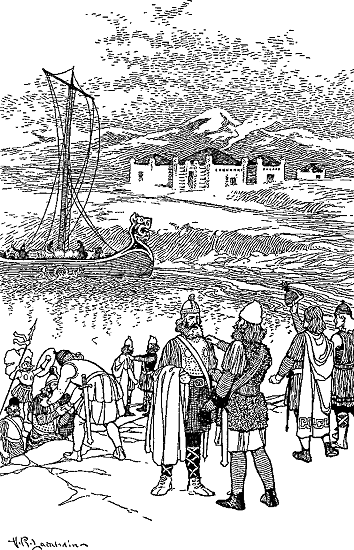
\includegraphics[width=9.1cm]{viking-tales/037}
    \caption{``Those Icelanders clapped them on the shoulders''}
\end{figure}

But after a while Ingolf led them to the feast hall and had a feast
spread at once. While the thralls were at work, the men stood together
and talked. Such a noise had never been in that hall before.

``We have already built our fires and claimed our land up the shore a
way,'' the leader said. ``Men in Norway talk much of Ingolf and Leif,
and wonder what has happened to them.''

Then Ingolf told them of all that had come to pass in Iceland; and then
he asked of Norway.

``Ah! things are going from bad to worse,'' the newcomers said. ``Harald
grows mightier every day. A man dare not swing a sword now except for
the king. We came here to get away from him. Many men are talking of
Iceland. Soon the sea-road between here and Norway will be swarming with
dragons.''

And so it was. Ships also came from Ireland and from the Shetlands and
the Orkneys.

``Harald has come west-over-seas,'' the men of these ships said, ``and
has laid his heavy hand upon the islands and put his earls over them.
They are no place now for free men.''

So by the time Ingolf was an old man, Iceland was no longer an empty
land. Every valley was spotted with bright feast halls and temples.
Horses and cattle pastured on the hillsides. Smoke curled up from
kitchens and smithies. Gay ships sailed the waters, taking Iceland cloth
and wool and Iceland fish and oil and the soft feathers of Iceland birds
to Norway to sell, and bringing back wood and flour and grain.

When Ingolf died, his men drew up on the shore the boat in which he had
come to Iceland. They painted it freshly and put new gold on it, so that
it stood there a glittering dragon with head raised high, looking over
the water. Old Sighvat lifted a huge stone and carried it to the ship's
side. With all his strength he threw it into the bottom. The timbers
cracked.

``If this ship moves from here,'' he said, ``then I do not know how to
moor a ship. It is Ingolf's grave.''

Then men laid Ingolf upon his shield and carried him and placed him on
the high deck in the stern near the pilot's seat where he had sat to
steer to Iceland. They hung his sword over his shoulder. They laid his
spear by his side. In his hand they put his mead-horn. Into the ship
they set a great treasure-chest filled with beautiful clothes and
bracelets and head-bands. Beside the treasure-chest they piled up many
swords and spears and shields. They put gold-trimmed saddles and bridles
upon three horses. Then they killed the horses and dragged them into the
ship. They killed hunting-dogs and put them by the horses; for they
said:

``All these things Ingolf will need in Valhalla. When he walks through
the door of that feast hall, Odin must know that a rich and brave man
comes. When he fights with those heroes during the day, he must have
weapons worthy of him. He must have dogs for the hunt. When he feasts
with those heroes at night he must wear rich clothes, so that those
feasters shall know that he was a wealthy man and generous, and that his
friends loved him.''

Ingolf's son tied on his hell-shoes for the long journey.

``If these shoes come untied,'' he said, ``I do not know how to fasten
hell-shoes.''

Then he went out of the ship and stood on the ground with his family.
All the men of Iceland were there.

``This is a glorious sight,'' they said. ``Surely no ship ever carried a
richer load. Inside and out the boat blazes with gold and bronze, and,
high over his riches, lies the great Ingolf, ready to take the tiller
and guide to Valhalla, where all the heroes will rise up and shout him
welcome.''

Then the thralls heaped a mound of earth over the ship. This hill stood
up against the sky and seemed to say: ``Here lies a great man.'' Sighvat
put a stone on the top, with runes on it telling whose grave it was. All
this time a skald stood by and played on his harp and sang a song about
that time when Ingolf came to Iceland. He called him the father of
Iceland. People of that country still read an old story that the men of
that long ago time wrote about Ingolf, and they love him because he was
a brave man and ``the first of men to come to Iceland.''

\begin{figure}[hb]
    \centering
    \vskip8pt
    
\includegraphics[width=2.7cm]{viking-tales/011}
\end{figure}

    \section[Eric the Red]{
    
\includegraphics[width=9.3cm]{viking-tales/038}\\
    Eric the Red}

\lettrine{I}{t} was a spring day many years after Ingolf died. All the
freemen in the west of Iceland had come to a meeting. Here they made laws
and punished men for having done wrong. The meeting was over now. Men
were walking about the plain and talking. Everybody seemed much excited.
Voices were loud, arms were swinging.

``It was an unjust decision,'' some one cried. ``Eric killed the men in
fair fight. The judges outlawed him because they were afraid. His foe
Thorgest has many rich and powerful men to back him.''

``No, no!'' said another. ``Eric is a bloody man. I am glad he is out of
Iceland.''

Just then a big man with bushy red hair and beard stalked through the
crowd. He looked straight ahead and scowled.

``There he goes,'' people said, and turned to look after him.

``His hands are as red as his beard,'' some said, and frowned.

But others looked at him and smiled, saying:

``He walks like Thor the Fearless.''

``His story would make a fine song,'' one said. ``As strong and as brave
and as red as Thor! Always in a quarrel. A man of many places--Norway,
the north of Iceland, the west of Iceland, those little islands off the
shore of Iceland. Outlawed from all of them on account of his quarrels.
Where will he go now, I wonder?''

This Eric strode down to the shore with his men following.

``He is in a black temper,'' they said. ``We should best not talk to
him.''

So they made ready the boat in silence. Eric got into the pilot's seat
and they sailed off. Soon they pulled the ship up on their own shore.
Eric strolled into his house and called for supper. When the
drinking-horns had been filled and emptied, Eric pulled himself up and
smiled and shouted out so that the great room was full of his big voice:

``There is no friend like mead. It always cheers a man's heart.''

\begin{figure}
    \centering
    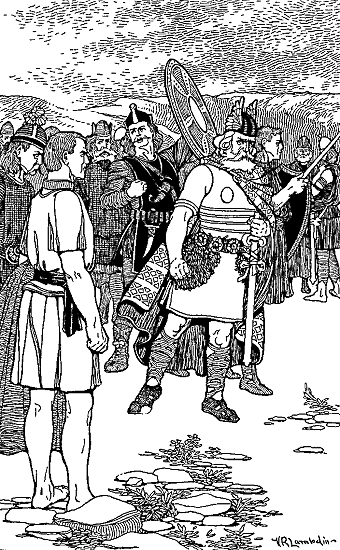
\includegraphics[width=9.1cm]{viking-tales/039}
    \caption{``He looked straight ahead of him and scowled''}
\end{figure}

Then laughter and talking began in the hall because Eric's good temper
had come back. After a while Eric said:

``Well, I must off somewhere. I have been driven about from place to
place, like a seabird in a storm. And there is always a storm about me.
It is my sword's fault. She is ever itching to break her
peace-bands\footnote{See note about peace-bands on
page~\pageref{peace-bands}.} and be out and at the play. She has shut
Norway to me and now Iceland. Where will you go next, old comrade?'' and
he pulled out his sword and looked at it and smiled as the fire flashed
on it.

``There are some of us who will follow you wherever you go, Eric,''
called a man from across the fire.

``Is it so?'' Eric cried, leaping up. ``Oh! then we shall have some
merry times yet. Who will go with me?''

More than half the men in the hall jumped to their feet and waved their
drinking-horns and shouted:

``I! I!''

\begin{figure}
    \centering
    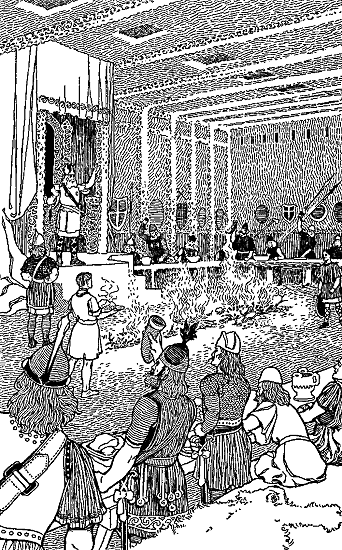
\includegraphics[width=9.1cm]{viking-tales/040}
    \caption{``ore than half the men in the hall jumped to their feet''}
\end{figure}

Eric sat down in his chair and laughed.

``O you bloody birds of battle!'' he cried. ``Ever hungry for new
frolic! Our swords are sisters in blood, and we are brothers in
adventure. Do you know what is in my heart to do?''

He jumped to his feet, and his face glowed. Then he laughed as he looked
at his men.

``I see the answer flashing from your eyes,'' he said, ``that you will
do it even if it is to go down to Niflheim and drag up Hela, the pale
queen of the stiff dead.''

His men pounded on the tables and shouted:

``Yes! Yes! Anywhere behind Eric!''

``But it is not to Niflheim,'' Eric laughed. ``Did you ever hear that
story that Gunnbiorn told? He was sailing for Iceland, but the fog came
down, and then the wind caught him and blew him far off. While he
drifted about he saw a strange land that rose up white and shining out
of a blue sea. Huge ships of ice sailed out from it and met him. I mean
to sail to that land.''

A great shout went up that shook the rafters. Then the men sat and
talked over plans. While they sat, a stranger came into the hall.

``I have no time to drink,'' he said. ``I have a message from your
friend Eyjolf. He says that Thorgest with all his men means to come here
and catch you to-night. Eyjolf bids you come to him, and he will hide
you until you are ready to start; for he loves you.''

``Hunted like a wolf from corner to corner of the world!'' Eric cried
angrily. ``Will they not even let me finish one feast?''

Then he laughed.

``But if I take my sport like a wolf, I must be hunted like one. So we
shall sleep to-night in the woods about Eyjolf's house, comrades,
instead of in these good beds. Well, we have done it before.''

``And it is no bad place,'' cried some of the men.

``I always liked the stars better than a smoky house fire,'' said one.

``Can no bad fortune spoil your good nature?'' laughed Eric. ``But now
we are off. Let every man carry what he can.''

So they quickly loaded themselves with clothes and gold and swords and
spears and kettles of food. Eric led his wife Thorhild and his two young
sons, Thorstein and Leif. All together they got into the boat and went
to Eyjolf's farm. For a week or more they stayed in his woods, sometimes
in a secret cave of his when they knew that Thorgest was about. And
sometimes Eyjolf sent and said:

``Thorgest is off. Come to my house for a feast.''

All this time they were making ready for the voyage, repairing the ship
and filling it with stores. Word of what Eric meant to do got out, and
men laughed and said:

``Is that not like Eric? What will he not do?''

Some men liked the sound of it, and they came to Eric and said:

``We will go with you to this strange land.''

So all were ready and they pushed off with Eric's family aboard and
those friends who had joined him. They took horses and cattle with them,
and all kinds of tools and food.

``I do not well know where this land is,'' Eric said. ``Gunnbiorn said
only that he sailed east when he came home to Iceland. So I will steer
straight west. We shall surely find something. I do not know, either,
how long we must go.''

So they sailed that strange ocean, never dreaming what might be ahead of
them. They found no islands to rest on. They met heavy fogs.

One day as Eric sat in the pilot's seat, he said:

``I think that I see one of Gunnbiorn's ships of ice. Shall we sail up
to her and see what kind of a craft she is?''

``Yes,'' shouted his men.

So they went on toward it.

``It sends out a cold breath,'' said one of the men.

They all wrapped their cloaks about them.

``It is a bigger boat than I ever saw before,'' said Eric. ``The white
mast stands as high as a hill.''

``It must be giants that sail in it, frost giants,'' said another of the
men.

But as they came nearer, Eric all at once laughed loudly and called out:

``By Thor, that Gunnbiorn was a foolish fellow. Why, look! It is only a
piece of floating ice such as we sometimes see from Iceland. It is no
ship, and there is no one on it.''

His men laughed and one called to another and said:

``And you thought of frost giants!''

Then they sailed on for days and days. They met many of these icebergs.
On one of them was a white bear.

``Yonder is a strange pilot,'' Eric laughed.

``I have seen bears come floating so to the north shore of Iceland,'' an
old man said. ``Perhaps they come from the land that we are going to
find.''

One day Eric said:

``I see afar off an iceberg larger than any one yet. Perhaps that is our
white land.''

\begin{figure}
    \centering
    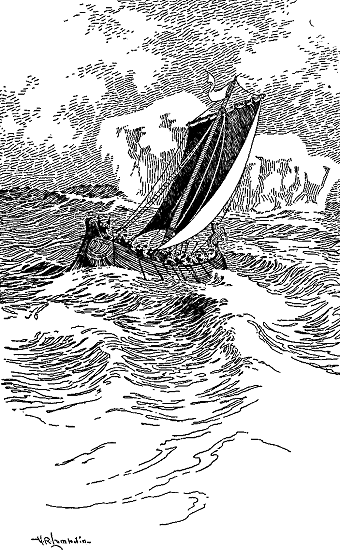
\includegraphics[width=9.1cm]{viking-tales/041}
    \caption{``It is a bigger boat than I ever saw before''}
\end{figure}

But even as he said it he felt his boat swing under his hand as he held
the tiller. He bore hard on the rudder, but he could not turn the ship.

``What is this?'' he cried. ``A strong river is running here. It is
carrying our ship away from this land. I cannot make head against it.
Out with the oars!''

So with oars and sail and rudder they fought against the current, but it
took the boat along like a chip, and after a while they put up their
oars and drifted.

``Luck has taken us into its own hands,'' Eric laughed. ``But this is as
good a way as another.''

Sometimes they were near enough to see the land, then they were carried
out into the sea and thought that they should never see any land again.

``Perhaps this river will carry us to a whirlpool and suck us under,''
the men said.

But at last Eric felt the current less strong under his hand.

``To the oars again!'' he called.

So they fought with the current and sailed out of it and went on toward
land. But when they reached the shore they found no place to go in.
Steep black walls shot up from the sea. Nothing grew on them. When the
men looked above the cliffs they saw a long line of white cutting the
sky.

``It is a land of ice,'' they said.

They sailed on south, all the time looking for a place to go ashore.

``I am sick of this endless sea,'' Thorhild complained, ``but this land
is worse.''

After a while they began to see small bays cut into the shore with
little flat patches of green at their sides. They landed in these places
and stretched and warmed themselves and ate.

``But these spots are only big enough for graves,'' the men said. ``We
can not live here.''

So they went on again. All the time the weather was growing colder.
Eric's people kept themselves wrapped in their cloaks and put scarfs
around their heads.

``And it is still summer!'' Thorhild said. ``What will it be in
winter?''

``We must find a place to build a house now before the winter comes
on,'' said Eric. ``We must not freeze here.''

So they chose a little spot with hills about it to keep off the wind.
They made a house out of stones; for there were many in that place. They
lived there that winter. The sea for a long way out from shore froze so
that it looked like white land. The men went out upon it to hunt white
bear and seal. They ate the meat and wore the skins to keep them warm.
The hardest thing was to get fuel for the fire. No trees grew there. The
men found a little driftwood along the shore, but it was not enough. So
they burned the bones and the fat of the animals they killed.

``It is a sickening smell,'' Thorhild said. ``I have not been out of
this mean house for weeks. I am tired of the darkness and the smoke and
the cattle. And all the time I hear great noises, as though some giant
were breaking this land into pieces.''

``Ah, cheer up, good wife!'' Eric laughed. ``I smell better luck
ahead.''

Once Eric and his men climbed the cliffs and went back into the middle
of the land. When they came home they had this to tell:

``It is a country of ice, shining white. Nothing grows on it but a few
mosses. Far off it looks flat, but when you walk upon it, there are
great holes and cracks. We could see nothing beyond. There seems to be
only a fringe of land around the edge of an island of ice.''

The winter nights were very long. Sometimes the sun showed for an hour,
sometimes for only a few minutes, sometimes it did not show at all for a
week. The men hunted by the bright shining of the moon or by the
northern lights.

As it grew warmer the ice in the sea began to crack and move and melt
and float away. Eric waited only until there was a clear passage in the
water. Then he launched his boat, and they sailed southward again. At
last they found a place that Eric liked.

``Here I will build my house,'' he said.

So they did and lived there that summer and pastured their cattle and
cut hay for the winter and fished and hunted.

The next spring Eric said:

``The land stretches far north. I am hungry to know what is there.''

Then they all got into the boat again and sailed north.

``We can leave no one here,'' Eric had said. ``We cannot tell what might
come between us. Perhaps giants or dragons or strange men might come out
of this inland ice and kill our people. We must stay together.''

Farther north they found only the same bare, frozen country. So after a
while they sailed back to their home and lived there.

One spring after they had been in that land for four years, Eric said:

``My eyes are hungry for the sight of men and green fields again. My
stomach is sick of seal and whale and bear. My throat is dry for mead.
This is a bare and cold and hungry land. I will visit my friends in
Iceland.''

``And our swords are rusty with long resting,'' said his men. ``Perhaps
we can find play for them in Iceland.''

``Now I have a plan,'' Eric suddenly said. ``Would it not be pleasant to
see other feast halls as we sail along the coast?''

``Oh! it would be a beautiful sight,'' his men said.

``Well,'' said Eric, ``I am going to try to bring back some neighbors
from Iceland. Now we must have a name for our land. How does Greenland
sound?''

His men laughed and said:

``It is a very white Greenland, but men will like the sound of it. It is
better than Iceland.''

So Eric and all his people sailed back and spent the winter with his
friends.

``Ah! Eric, it is good to hear your laugh again,'' they said.

Eric was at many feasts and saw many men, and he talked much of his
Greenland.

``The sea is full of whale and seals and great fish,'' he said. ``The
land has bear and reindeer. There are no men there. Come back with me
and choose your land.''

Many men said that they would do it. Some men went because they thought
it would be a great frolic to go to a new country. Some went because
they were poor in Iceland and thought:

``I can be no worse off in Greenland, and perhaps I shall grow rich
there.''

And some went because they loved Eric and wanted to be his neighbors.

So the next summer thirty-five ships full of men and women and goods
followed Eric for Greenland. But they met heavy storms, and some ships
were wrecked, and the men drowned. Other men grew heartsick at the
terrible storm and the long voyage and no sight of land, and they turned
back to Iceland. So of those thirty-five ships only fifteen got to
Greenland.

``Only the bravest and the luckiest men come here,'' Eric said. ``We
shall have good neighbors.''

Soon other houses were built along the fiords.

``It is pleasant to sail along the coast now,'' said Eric. ``I see smoke
rising from houses and ships standing on the shore and friendly hands
waving.''

    \section[Leif and His New Land]{
    
\includegraphics[width=9.3cm]{viking-tales/042}\\
    Leif and His New Land}

\lettrine{N}{ow} Eric had lived in Greenland for fifteen years. His sons
Thorstein and Leif had grown up to be big, strong men. One spring Leif
said to his father:

``I have never seen Norway, our mother land. I long to go there and meet
the great men and see the places that skalds sing about.''

Eric answered:

``It is right that you should go. No man has really lived until he has
seen Norway.''

So he helped Leif fit out a boat and sent him off. Leif sailed for
months. He passed Iceland and the Faroes and the Shetlands. He stopped
at all of these places and feasted his mind on the new things. And
everywhere men received him gladly; for he was handsome and wise. But at
last he came near Norway. Then he stood up before the pilot's seat and
sang loudly:

\begin{quote}
``My eyes can see her at last,\\
The mother of mighty men,\\
The field of famous fights.\\
In the sky above I see\\
Fair Asgard's shining roofs,\\
The flying hair of Thor,\\
The wings of Odin's birds,\\
The road that heroes tread.\\
I am here in the land of the gods,\\
The land of mighty men.''
\end{quote}

For a while he walked the land as though he were in a dream. He looked
at this and that and everything and loved them all because it was
Norway.

``I will go to the king,'' he said.

He had never seen a king. There were no kings in Iceland or in
Greenland. So he went to the city where the king had his fine house. The
king's name was Olaf. He was a great-grandson of Harald Hairfair; for
Harald had been dead a hundred years.

Now the king was going to hold a feast at night, and Leif put on his
most beautiful clothes to go to it. He put on long tights of blue wool
and a short jacket of blue velvet. He belted his jacket with a gold
girdle. He had shoes of scarlet with golden clasps. He threw around
himself a cape of scarlet velvet lined with seal fur. His long sword
stuck out from under his cloak. On his head he put a knitted cap of
bright colors. Then he walked to the king's feast hall and went through
the door. It was a great hall, and it was full of richly-dressed men.
The fires shone on so many golden head-bands and bracelets and so many
glittering swords and spears on the wall, and there was so much noise of
talking and laughing, that at first Leif did not know what to do. But at
last he went and sat on the very end seat of the bench near him.

As the feast went on, King Olaf sat in his high seat and looked about
the hall and noticed this one and that one and spoke across the fire to
many. He was keen-eyed and soon saw Leif in his far seat.

``Yonder is some man of mark,'' he said to himself. ``He is surely worth
knowing. His face is not the face of a fool. He carries his head like a
lord of men.''

He sent a thrall and asked Leif to come to him. So Leif walked down the
long hall and stood before the king.

``I am glad to have you for a guest,'' the king said. ``What are your
name and country?''

``I am Leif Ericsson, and I have come all the way from Greenland to see
you and old Norway.''

``From Greenland!'' said the king. ``It is not often that I see a
Greenlander. Many come to Norway to trade, but they seldom come to the
king's hall. I shall be glad to hear about your land. Come up and speak
with me.''

So Leif went up the steps of the high seat and sat down by the king and
talked with him. When the feast was over the king said:

``You shall live at my court this winter, Leif Ericsson. You are a
welcome guest.''

So Leif stayed there that winter. When he started back in the spring,
the king gave him two thralls as a parting gift.

``Let this gift show my love, Leif Ericsson,'' he said. ``For your sake
I shall not forget Greenland.''

Leif sailed back again and had good luck until he was past Iceland. Then
great winds came out of the north and tossed his ship about so that the
men could do nothing. They were blown south for days and days. They did
not know where they were. Then they saw land, and Leif said:

``Surely luck has brought us also to a new country. We will go in and
see what kind of a place it is.''

So he steered for it. As they came near, the men said:

``See the great trees and the soft, green shore. Surely this is a better
country than Greenland or than Iceland either.''

When they landed they threw themselves upon the ground.

``I never lay on a bed so soft as this grass,'' one said.

``Taller trees do not grow in Norway,'' said another.

``There is no stone here as in Norway, but only good black dirt,'' Leif
said. ``I never saw so fertile a land before.''

The men were hungry and set about building a fire.

``There is no lack of fuel here,'' they said.

They stayed many days in this country and walked about to see what was
there. A German, named Tyrker, was with Leif. He was a little man with a
high forehead and a short nose. His eyes were big and rolling. He had
lived with Eric for many years, and had taken care of Leif when he was a
little boy. So Leif loved him.

Now one day they had been wandering about and all came back to camp at
night except Tyrker. When Leif looked around on his comrades, he said:

``Where is Tyrker?''

No one knew. Then Leif was angry.

``Is a man of so little value in this empty land that you would lose
one?'' he said. ``Why did you not keep together? Did you not see that he
was gone? Why did you not set out to look for him? Who knows what
terrible thing may have happened to him in these great forests?''

Then he turned and started out to hunt for him. His men followed, silent
and ashamed. They had not gone far when they saw Tyrker running toward
them. He was laughing and talking to himself. Leif ran to him and put
his arms about him with gladness at seeing him.

\begin{figure}
    \centering
    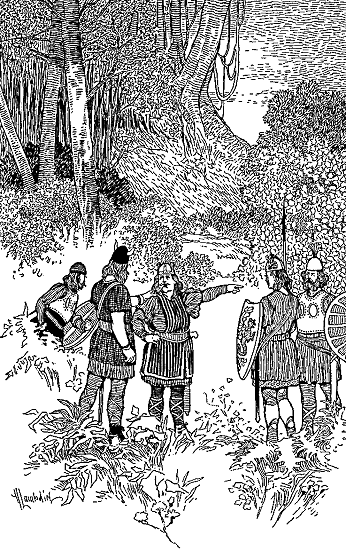
\includegraphics[width=9.1cm]{viking-tales/043}
    \caption{``He pointed to the woods and laughed and rolled his eyes''}
\end{figure}

``Why are you so late?'' he asked. ``Where have you been?''

But Tyrker, still smiling and nodding his head, answered in German. He
pointed to the woods and laughed and rolled his eyes. Again Leif asked
his question and put his hand on Tyrker's shoulder as though he would
shake him. Then Tyrker answered in the language of Iceland:

``I have not been so very far, but I have found something wonderful.''

``What is it?'' cried the men.

``I have found grapes growing wild,'' answered Tyrker, and he laughed,
and his eyes shone.

``It cannot be,'' Leif said.

Grapes do not grow in Greenland nor in Iceland nor even in Norway. So it
seemed a wonderful thing to these Norsemen.

``Can I not tell grapes when I see them?'' cried Tyrker. ``Did I not
grow up in Germany, where every hillside is covered with grapevines? Ah!
it seems like my old home.''

``It is wonderful,'' Leif said. ``I have heard travelers tell of seeing
grapes growing, but I myself never saw it. You shall take us to them
early in the morning, Tyrker.''

So in the morning they went back into the woods and saw the grapes. They
ate of them.

``They are like food and drink,'' they cried.

That day Leif said:

``We spent most of the summer on the ocean. Winter will soon be coming
on and the sea about Greenland will be frozen. We must start back. I
mean to take some of the things of this land to show to our people at
home. We will fill the rowboat with grapes and tow it behind us. The
ship we will load with logs from these great trees. That will be a
welcome shipload in Greenland, where we have neither trees nor vines.
Now half of you shall gather grapes for the next few days, and the other
half shall cut timber.''

So they did, and after a week sailed off. The ship was full of lumber,
and they towed the rowboat loaded with grapes. As they looked back at
the shore, Leif said:

``I will call this country Wineland for the grapes that grow there.''

One of the men leaped upon the gunwale and leaned out, clinging to the
sail, and sang:

\begin{quote}
``Wineland the good, Wineland the warm,\\
Wineland the green, the great, the fat.\\
Our dragon fed and crawls away\\
With belly stuffed and lazy feet.\\
How long her purple, trailing tail!\\
She fed and grew to twice her size.''
\end{quote}

Then all the men waved their hands to the shore and gave a great shout
for that good land.

For all that voyage they had fair weather and sailed into Eric's harbor
before the winter came. Eric saw the ship and ran down to the shore. He
took Leif into his arms and said:

``Oh, my son, my old eyes ached to see you. I hunger to hear of all that
you have seen and done.''

``Luck has followed me all the way,'' said Leif. ``See what I have
brought home.''

The Greenlanders looked.

``Lumber! lumber!'' they cried. ``Oh! it is better stuff than gold.''

Then they saw the grapes and tasted them.

``Surely you must have plundered Asgard,'' they said, smacking their
lips.

At the feast that night Eric said:

``Leif shall sit in the place of honor.''

So Leif sat in the high seat opposite Eric. All men thought him a
handsome and wise man. He told them of the storm and of Wineland.

``No man would ever need a cloak there. The soil is richer than the soil
of Norway. Grain grows wild, and you yourselves saw the grapes that we
got from there. The forests are without end. The sea is full of fish.''

The Greenlanders listened with open mouths to all this. They turned and
talked to Leif's ship-comrades who were scattered among them.

Leif noticed two strangers, an old man who sat at Eric's side and a
young woman on the cross-bench. He turned to his brother Thorstein who
sat next to him.

``Who are these strangers?'' he asked.

``Thorbiorn and his daughter Gudrid,'' Thorstein answered. ``They landed
here this spring. I never saw our father more glad of anything than to
see this Thorbiorn. They were friends before we left Iceland. When they
saw each other again they could not talk enough of old times. In the
spring Eric means to give him a farm up the fiord a way. It seems that
this Thorbiorn comes of a good family that has been rich and great in
Iceland for years. And Thorbiorn himself was rich when our father knew
him, and was much honored by all men. But ill luck came, and he grew
poor. This hurt his pride. `I will not stay in Iceland and be a beggar,'
he said to himself. `I will not have men look at me and say, ``He is not
what his father was.'' I will go to my friend Eric the Red in
Greenland.'

``Then he got ready a great feast and invited all his friends. It was
such a feast as had not been in Iceland for years. Thorbiorn spent on it
all the wealth that he had left. For he said to himself, `I will not
leave in shame. Men shall remember my last feast.' After that he set out
and came to Greenland.

``Is not Gudrid beautiful? And she is wise. I mean to marry her, if her
father will permit it.''

Now Leif settled down in Greenland and became a great man there. He was
so busy and he grew so rich that he did not think of going to Wineland
again. But people could not forget his story. Many nights as men sat
about the long fires they talked of that wonderful land and wished to
see it.

\begin{figure}[hb]
    \centering
    \vskip8pt
    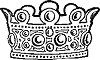
\includegraphics[width=2.7cm]{viking-tales/014}
\end{figure}

    \chapter[Wineland the Good]{
    
\includegraphics[width=9.3cm]{viking-tales/044}\\
    Wineland the Good}

\lettrine{O}{n} an autumn, a year or two after Leif came home, Eric and
his men saw two large ships come to land not far down the shore from the
house.

``They look like trading ships,'' Eric said. ``Let us go down to see
them.''

``I will go, too,'' Gudrid said. ``Perhaps they will have rich cloth and
jewelry. It is long since I had my eyes on a new dress.''

So they all went down and found two large trading ships lying in the
water. A great many men were on the shore making a fire.

``Welcome to Greenland!'' called Eric. ``What are your names and your
country?''

Then a fine, big man walked out from among the men and went up to Eric.

``I am Thorfinn,'' he said, ``a trader. I sailed this summer from
Iceland with forty men and a shipload of goods. On the sea I met this
other ship from Iceland. The master is Biarni. Come and look at my
goods.''

So he rowed Eric and Gudrid out and they went aboard his boat. Thorfinn
opened his chests and showed Eric gleaming swords and bracelets and axes
and farm tools. But before Gudrid he spread beautiful cloth and gold
embroidery and golden necklaces. As they looked, he told of doings in
Iceland and asked of Greenland.

``We never see such things as these in this bare land,'' Gudrid said, as
she smoothed a beautiful dress of purple velvet. ``I envy the women of
Iceland their fair clothes.''

``There is no need of that,'' Thorfinn said, ``for this dress is yours
and anything else from my chests that you like. Here is a necklace that
I beg you to take. It did not have a fairer mistress in Greece where I
got it.''

``You are a very generous trader,'' Gudrid said.

Then Thorfinn gave Eric a great sword with a gold-studded scabbard.
After a while he took them to Biarni's ship. He also gave them gifts.
They all talked and laughed much while they were together.

``You are merry comrades,'' Eric said. ``I ask you both and all your men
to spend the winter at my house. You can put your goods into my
storehouses.''

``By my sword! a generous offer,'' said Thorfinn. ``As for me, I am
happy to come.''

Biarni and all the rest said the same thing. Thorfinn walked to the
house with Eric and Gudrid, while the other men sailed to the ship-sheds
and pulled their boats under them.

Then Thorfinn saw to the unloading and storing of his goods.

``Is this Gudrid your daughter?'' he asked of Eric one day.

``She is the widow of my son Thorstein,'' Eric said. ``He died the same
winter that they were married. Her father, too, died not long ago. So
Gudrid lives with me.''

Now all that winter until Yule-time Eric spread a good feast every
night. There was laughter through his house all the time. Often at the
feasts the men cast lots to see whether they might sit on the
cross-bench with the women. Sometimes it was Thorfinn's luck to sit by
Gudrid. Then they talked gaily and drank together.

At last Yule was coming near. Eric went about the house gloomy then. One
day Thorfinn put his hand on Eric's shoulder and said:

``Something is troubling you, Eric. We have all noticed that you are not
gay as you used to be. Tell me what is the matter.''

``You have carried yourselves like noble men in my house,'' Eric
answered. ``I am proud to have you for guests. Now I am ashamed that you
should not find a house worthy of you. I am ashamed that when you leave
me you will have to say that you never spent a worse Yule than you did
with Eric the Red in Greenland. For my cupboards are empty.''

``Oh, that is easily mended,'' Thorfinn said. ``No house could feed
eighty men so long and not feel it. I never knew so generous a host
before. But I have flour and grain and mead in my boat. You are welcome
to all of it. You have only to open the doors of your own storehouses.
It is a little gift.''

So Eric used those things, and there was never a merrier Yule feast than
in his house that winter.

When Yule was over, Thorfinn said to Eric:

``Gudrid is a beautiful and wise woman. I wish to have her for my
wife.''

``You seem to be a man worthy of her,'' Eric said.

So that winter Gudrid and Thorfinn were married and lived at Eric's
house.

One day Thorfinn said to Eric:

``I have heard much of this wonderful Wineland since I have been here.
It seems to me that it is worth while to go and see more of it.''

``My son Thorstein and I tried it once,'' said Eric. ``It was the year
after Leif came back. We set out with a fair ship and with glad hearts,
but we tossed about all summer on the sea and got nowhere. We were wet
with storm, lean with hunger and illness, and heartsick at our bad
luck.''

``And yet,'' Thorfinn said, ``another time we might have better weather.
I have never seen so fair a land as this seems to be.''

Then he went to Leif and talked long with him. Leif told him in what
direction he had sailed to come home, and how the shores looked that he
had passed.

``I think I could find my way,'' Thorfinn said. ``My heart moves me to
try this frolic.''

He spoke to Gudrid about it.

``Oh, yes!'' she cried. ``Let us go. It is long since I felt a boat
leaping under me. I am tired of sitting still. I want to feel the warm
days and see the soft grass and the high trees and taste the grapes of
this Wineland the Good.''

Then he talked with his men and with Biarni.

``We are ready,'' they all said. ``We are only waiting for a leader.''

``Then let us go!'' cried Thorfinn.

So in the spring they fitted up their two ships and put into them
provisions and a few cattle. Some of Eric's men also got ready a boat,
so that three ships set sail from Eric's harbor carrying one hundred and
sixty men to Wineland. As they started, Gudrid stood on the deck and
sang:

\begin{quote}
``I will feast my eyes on new things--\\
On mighty trees and purple grapes,\\
On beds of flowers and soft grass.\\
I will sun myself in a warm land.''
\end{quote}

They sailed on and past those shores that Leif had spoken of. Whenever
they saw any interesting place they sailed in and looked about and
rested there.

They had gone far south, past many fair shores with woods on them, when
Gudrid said one day:

``This is a beautiful bay with a smooth, green field by it, and the
great mountains far back. I should like to stay there for a little
while.''

So they sailed in and drew their ships up on shore. They put up the
awnings in them.

``These shall be our houses,'' Thorfinn said.

They were strange-looking houses--shining dragons with gay backs lying
on the yellow sand. Near them the Norsemen lighted fires and cooked
their supper. That night they slept in the ships. In the morning Gudrid
said:

``I long to see what is back of that mountain.''

So they all climbed it. When they stood on the top they could see far
over the country.

``There is a lake that we must see,'' Thorfinn said.

``I should like to sail around that bay,'' said Biarni, pointing.

``I am going to walk up that valley yonder,'' one of the men said.

And everyone saw some place where he would like to go. So for all that
summer they camped in that spot and went about the country seeing new
things. They hunted in the woods and caught rabbits and birds and
sometimes bears and deer. Every day some men rowed out to sea and
fished. There was an island in the bay where thousands of birds had
their nests. The men gathered eggs here.

``We have more to eat than we had in Greenland or Iceland,'' Thorfinn
said, ``and need not work at all. It is all play.''

Near the end of summer Thorfinn spoke to his comrades.

``Have we not seen everything here? Let us go to a new place. We have
not yet found grapes.''

Thorfinn and Biarni and all their men sailed south again. But some of
Eric's men went off in their boat another way. Years afterward the
Greenlanders heard that they were shipwrecked and made slaves in
Ireland.

After Thorfinn and Biarni had sailed for many days they landed on a low,
green place. There were hills around it. A little lake was there.

``What is growing on those hillsides?'' Thorfinn said, shading his eyes
with his hand.

He and some others ran up there. The people on shore heard them shout.
Soon they came running back with their hands full of something.

``Grapes! Grapes!'' they were shouting.

All those people sat down and ate the grapes and then went to the
hillside and picked more.

``Now we are indeed in Wineland,'' they said. ``It is as wonderful as
Leif's stories. Surely we must stay here for a long time.''

The very next day they went into the woods and began to cut out lumber.
The huts that they built were little things. They had no windows, and in
the doorways the men hung their cloaks instead of doors.

``We can be out in the air so much in this warm country,'' said Gudrid,
``that we do not need fine houses.''

The huts were scattered all about, some on the side of the lake, some at
the shore of the harbor, some on the hillside. Gudrid had said:

``I want to live by the lake where I can look into the green woods and
hear sweet bird-noises.''

So Thorfinn built his hut there.

As they sat about the campfire one night, Biarni said:

``It is strange that so good a land should be empty. I suppose that
these are the first houses that were ever built in Wineland. It is
wonderful to think that we are alone here in this great land.''

All that winter no snow fell. The cattle pastured on the grass.

``To think of the cold, frozen winters in Greenland!'' Gudrid said.
``Oh! this is the sun's own land.''

In the beginning of that winter a little son was born to Gudrid and
Thorfinn.

``A health to the first Winelander!'' the men shouted and drank down
their wine; for they had made some from Wineland grapes.

``Will he be the father of a great country, as Ingolf was?'' Biarni
mused.

Gudrid looked at her baby and smiled.

``You will be as sunny as this good land, I hope,'' she said.

They named him Snorri. He grew fast and soon crept along the yellow
sand, and toddled among the grapevines, and climbed into the boats and
learned to talk. The men called him the ``Wineland king.''

``I never knew a baby before,'' one of the men said.

``No,'' said another. ``Swords are jealous. But when they are in their
scabbards, we can do other things, even play with babies.''

``I wonder whether I have forgotten how to swing my sword in this quiet
land,'' another man said.

One spring morning when the men got up and went out from their huts to
the fires to cook they saw a great many canoes in the harbor. Men were
in them paddling toward shore.

``What is this?'' cried the Norsemen to one another. ``Where did they
come from? Are they foes? Who ever saw such boats before? The men's
faces are brown.''

``Let every man have his sword ready,'' cried Thorfinn. ``But do not
draw until I command. Let us go to meet them.''

So they went and stood on the shore. Soon the men from the canoes landed
and stood looking at the Norsemen. The strangers' skin was brown. Their
faces were broad. Their hair was black. Their bodies were short. They
wore leather clothes. One man among them seemed to be chief. He spread
out his open hands to the Norsemen.

``He is showing us that he has no weapons,'' Biarni said. ``He comes in
peace.''

Then Thorfinn showed his empty hands and asked:

``What do you want?''

The stranger said something, but the Norsemen could not understand. It
was some new language. Then the chief pointed to one of the huts and
walked toward it. He and his men walked all around it and felt of the
timber and went into it and looked at all the things there--spades and
cloaks and drinking-horns. As they looked they talked together. They
went to all the other huts and looked at everything there. One of them
found a red cloak. He spread it out and showed it to the others. They
all stood about it and looked at it and felt of it and talked fast.

``They seem to like my cloak,'' Biarni said.

One of the strangers went down to their canoes and soon came back with
an armload of furs--fox-skins, otter-skins, beaver-skins. The chief took
some and held them out to Thorfinn and hugged the cloak to him.

\begin{figure}
    \centering
    \includegraphics[width=9.1cm]{viking-tales/045}
    \caption{``The chief held them out to Thorfinn and hugged the cloak
        to him''}
\end{figure}

``He wants to trade,'' Thorfinn said. ``Will you do it, Biarni?''

``Yes,'' Biarni answered, and took the furs.

``If they want red stuff, I have a whole roll of red cloth that I will
trade,'' one of the other men said.

He went and got it. When the strangers saw it they quickly held out more
furs and seemed eager to trade. So Thorfinn cut the cloth into pieces
and sold every scrap. When the strangers got it they tied it about their
heads and seemed much pleased.

While this trading was going on and everybody was good-natured, a bull
of Thorfinn's ran out of the woods bellowing and came towards the crowd.
When the strangers heard it and saw it they threw down whatever was in
their hands and ran to their canoes and paddled off as fast as they
could.

The Norsemen laughed.

``We have lost our customers,'' Biarni said.

``Did they never see a bull before?'' laughed one of the men.

Now after three weeks the Norsemen saw canoes in the bay again. This
time it was black with them, there were so many. The people in them were
all making a horrible shout.

``It is a war-cry,'' Thorfinn said, and he raised a red shield. ``They
are surely twenty to our one, but we must fight. Stand in close line and
give them a taste of your swords.''

Even as he spoke a great shower of stones fell upon them. Some of the
Norsemen were hit on the head and knocked down. Biarni got a broken arm.
Still the storm came fast. The strangers had landed and were running
toward the Norsemen. They threw their stones with sling-shots, and they
yelled all the time.

``Oh, this is no kind of fighting for brave men!'' Thorfinn cried
angrily.

The Norsemen's swords swung fast, and many of the strangers died under
them, but still others came on, throwing stones and swinging stone axes.
The horrible yelling and the strange things that the savages did
frightened the Norsemen.

``These are not men,'' some one cried.

Then those Norsemen who had never been afraid of anything turned and
ran. But when they came to the top of a rough hill Thorfinn cried:

``What are we doing? Shall we die here in this empty land with no one to
bury us? We are leaving our women.''

Then one of the women ran out of the hut where they were hiding.

``Give me a sword!'' she cried. ``I can drive them back. Are Norsemen
not better than these savages?''

Then those warriors stopped, ashamed, and stood up before the wild men
and fought so fiercely that the strangers turned and fled down to their
canoes and paddled away.

``Oh, I am glad they are gone!'' Thorfinn said. ``It was an ugly
fight.''

``Thor would not have loved that battle,'' one said.

``It was no battle,'' another replied. ``It was like fighting against an
army of poisonous flies.''

The Norsemen were all worn and bleeding and sore. They went to their
huts and dressed their wounds, and the women helped them. At supper that
night they talked about the fight for a long time.

``I will not stay here,'' Gudrid said. ``Perhaps these wild men have
gone away to get more people and will come back and kill us. Oh! they
are ugly.''

``Perhaps brown faces are looking at us now from behind the trees in the
woods back there,'' said Biarni.

It was the wish of all to go home. So after a few days they sailed back
to Greenland with good weather all the way. The people at Eric's house
were very glad to see them.

``We were afraid you had died,'' they said.

``And I thought once that we should never leave Wineland alive,''
Thorfinn answered.

Then they told all the story.

``I wonder why I had no such bad luck,'' Leif said. ``But you have a
better shipload than I got.''

He was looking at the bundles of furs and the kegs of wine.

``Yes,'' said Thorfinn, ``we have come back richer than when we left.
But I will never go again for all the skins in the woods.''

The next summer Thorfinn took Gudrid and Snorri and all his people and
sailed back to Iceland, his home. There he lived until he died. People
looked at him in wonder.

``That is the man who went to Wineland and fought with wild men,'' they
said. ``Snorri is his son. He is the first and last Winelander, for no
one will ever go there again. It will be an empty and forgotten land.''

And so it was for a long time. Some wise men wrote down the story of
those voyages and of that land, and people read the tale and liked it,
but no one remembered where the place was. It all seemed like a fairy
tale. Long afterwards, however, men began to read those stories with
wide-open eyes and to wonder. They guessed and talked together, and
studied this and that land, and read the story over and over. At last
they have learned that Wineland was in America, on the eastern shore of
the United States, and they have called Snorri the first American, and
have put up statues of Leif Ericsson, the first comer to
America.\footnote{See note about eskimos on page~\pageref{eskimos}.}

\begin{figure}[hb]
    \centering
    \vskip8pt
    \includegraphics[width=2.7cm]{viking-tales/017}
\end{figure}


    \backmatter
    \appendix
    % add vertical space in toc
    \addtocontents{toc}{\vspace{\cftbeforechapskip}}
    \section[Descriptive Notes]{
    \includegraphics[width=9.3cm]{viking-tales/046}}

\phantomsection\label{house}
\emph{House.} In a rich Norseman's home were many buildings. The finest
and largest was the great feast hall. Next were the bower, where the
women worked, and the guest house, where visitors slept. Besides these
were storehouses, stables, work-shops, a kitchen, a sleeping-house for
thralls. All these buildings were made of heavy, hewn logs, covered with
tar to fill the cracks and to keep the wood from rotting. The ends of
the logs, the door-posts, the peaks of gables, were carved into shapes
of men and animals and were painted with bright colors. These gay
buildings were close together, often set around the four sides of a
square yard. That yard was a busy and pleasant place, with men and women
running across from one bright building to another. Sometimes a high
fence with one gate went around all this, and only the tall, carved
peaks of roofs showed from the outside.

\phantomsection\label{names}
\noindent\emph{Names.} An old Norse story says: ``Most men had two names
in one, and thought it likeliest to lead to long life and good luck to
have double names.'' To be called after a god was very lucky. Here are
some of those double names with their meanings: ``Thorstein'' means
Thor's stone; ``Thorkel'' means Thor's fire; ``Thorbiorn'' means Thor's
bear; ``Gudbrand'' means Gunnr's sword (Gunnr was one of the
Valkyrias\footnote{See note about Valkyrias on
page~\pageref{valkyrias}.}); ``Gunnbiorn'' means Gunnr's bear; ``Gudrid''
means Gunnr's rider; ``Gudrod'' means Gunnr's land-clearer. (Most of the
land in old Norway was covered with forests. When a man got new land he
had to clear off the trees.) In those olden days a man did not have a
surname that belonged to everyone in his family. Sometimes there were
two or three men of the same name in a neighborhood. That caused
trouble. People thought of two ways of making it easy to tell which man
was being spoken of. Each was given a nickname. Suppose the name of each
was Haki. One would be called Haki the Black because he had black hair.
The other would be called Haki the Ship-chested because his chest was
broad and strong. These nicknames were often given only for the fun of
it. Most men had them,--Eric the Red, Leif the Lucky, Harald Hairfair,
Rolf Go-afoot. The other way of knowing one Haki from the other was to
tell his father's name. One was Haki, Eric's son. The other was Haki,
Halfdan's son. If you speak these names quickly, they sound like Haki
Ericsson and Haki Halfdansson. After a while they were written like
that, and men handed them on to their sons and daughters. Some names
that we have nowadays have come down to us in just that way--Swanson,
Anderson, Peterson, Jansen. There was another reason for these last
names: a man was proud to have people know who his father was.

\phantomsection\label{drinking-horns}
\noindent\emph{Drinking-horns.} The Norsemen had few cups or goblets.
They used instead the horns of cattle, polished and trimmed with gold or
silver or bronze. They were often very beautiful, and a man was almost as
proud of his drinking-horn as of his sword.

\phantomsection\label{tables}
\noindent\emph{Tables.} Before a meal thralls brought trestles into the
feast hall and set them before the benches. Then they laid long boards
across from trestle to trestle. These narrow tables stretched all along
both sides of the hall. People sat at the outside edge only. So the
thralls served from the middle of the room. They put baskets of bread and
wooden platters of meat upon these bare boards. At the end of the meal
they carried out tables and all, and the drinking-horns went round in a
clean room.

\phantomsection\label{beds}
\noindent\emph{Beds.} Around the sides of the feast hall were shut-beds.
They were like big boxes with doors opening into the hall. On the floor
of this box was straw with blankets thrown over it. The people got into
these beds and closed the doors and so shut themselves in. Olaf's men
could have set heavy things against these doors or have put props
against them. Then the people could not have got out; for on the other
side of the bed was the thick outside wall of the feast hall, and there
were no windows in it.

\phantomsection\label{feast-hall}
\noindent\emph{Feast Hall.} The feast hall was long and narrow, with a
door at each end. Down the middle of the room were flat stones in the
dirt floor. Here the fires burned. In the roof above these fires were
holes for the smoke to go out, but some of it blew about the hall, and
the walls and rafters were stained with it. But it was pleasant wood
smoke, and the Norsemen did not dislike it. There were no large windows
in a feast hall or in any other Norse building. High up under the eaves
or in the roof itself were narrow slits that were called wind's-eyes.
There was no glass in them, for the Norsemen did not know how to make it;
but there were, instead, covers made of thin, oiled skin. These were put
into the wind's-eyes in stormy weather. There were covers, too, for the
smoke-holes. The only light came through these narrow holes, so on dark
days the people needed the fire as much for light as for warmth.

\phantomsection\label{foster-father}
\noindent\emph{Foster-father.} A Norse father sent his children away from
home to grow up. They went when they were three or four years old and
stayed until they were grown. The father thought: ``They will be better
so. If they stayed at home, their mother would spoil them with much
petting.''

\phantomsection\label{foster-brothers}
\noindent\emph{Foster-brothers.} When two men loved each other very much
they said, ``Let us become foster-brothers.''

Then they went and cut three long pieces of turf and put a spear into
the ground so that it held up the strips of turf like an arch. Runes
were cut on the handle of the spear, telling the duties of
foster-brothers. The two men walked under this arch, and each made a
little cut in his palm. They knelt and clasped hands, so that the blood
of the two flowed together, and they said, ``Now we are of one blood.''

Then each made this vow: ``I will fight for my foster-brother whenever
he shall need me. If he is killed before I am, I will punish the man who
did it. Whatever things I own are as much my foster-brother's as mine. I
will love this man until I die. I call Odin and Thor and all the gods to
hear my vow. May they hate me if I break it!''

\phantomsection\label{ran}
\noindent\emph{Ran.} Ran was the wife of Aegir, who was god of the sea.
They lived in a cave at the bottom of the ocean. Ran had a great net, and
she caught in it all men who were shipwrecked and took them to her cave.
She also caught all the gold and rich treasures that went down in ships.
So her cave was filled with shining things.

\phantomsection\label{valkyrias}
\noindent\emph{Valkyrias.} These were the maidens of Odin. They waited
on the table in Valhalla. But whenever a battle was being fought they
rode through the air on their horses and watched to see what warriors
were brave enough to go to Valhalla. Sometimes during the fight a man
would think that he saw the Valkyrias. Then he was glad; for he knew that
he would go to Valhalla.

An old Norse story says this about the Valkyrias: ``With lightning
around them, with bloody shirts of mail, and with shining spears they
ride through the air and the ocean. When their horses shake their manes,
dew falls on the deep valleys and hail on the high forests.''

\phantomsection\label{odins-ravens}
\noindent\emph{Odin's Ravens.} Odin had a great throne in his palace in
Asgard. When he sat in it he could look all over the world. But it was so
far to see that he could not tell all of the things that were happening.
So he had two ravens to help him. An old Norse story tells this about
them: ``Two ravens sit on Odin's shoulders and whisper in his ears all
that they have heard and seen. He sends them out at dawn of day to see
over the whole world. They return at evening near meal time. This is why
Odin knows so many things.''

\phantomsection\label{reykjavik}
\noindent\emph{Reykjavik.} Reykjavik means ``smoky sea.'' Ingolf called
it that because of the steaming hot-springs by the sea. The place is
still called Reykjavik. A little city has grown up there, the only city
in Iceland. It is the capital of the country.

\phantomsection\label{peace-bands}
\noindent\emph{Peace-bands.} A Norseman always carried his sword, even at
a feast; for he did not know when he might need it. But when he went
somewhere on an errand of peace and had no quarrel he tied his sword
into its scabbard with white bands that he called peace-bands. If all at
once something happened to make him need his sword, he broke the
peace-bands and drew it out.

\phantomsection\label{eskimos}
\noindent\emph{Eskimos.} Now, the Eskimos live in Greenland and Alaska
and on the very northern shores of Canada. But once they lived farther
south in pleasanter lands. After a while the other Indian tribes began to
grow strong. Then they wanted the pleasant land of the Eskimos and the
seashore that the Eskimos had. So they fought again and again with those
people and won and drove them farther north and farther north. At last
the Eskimos were on the very shores of the cold sea, with the Indians
still pushing them on. So some of them got into their boats and rowed
across the narrow water and came to Greenland and lived there. Some
people think that these things happened before Eric found Greenland. In
that case he found Eskimos there; and Thorfinn saw red Indians in
Wineland. Other people think that this happened after Eric went to
Greenland. If that is true, he found an empty land, and it was Eskimos
that Thorfinn saw in Wineland.

\section[Suggestions to Teachers]{
    \includegraphics[width=9.3cm]{viking-tales/047}}

\lettrine{P}{ossibly} this book seems made up of four or five
disconnected stories. They are, however, strung upon one thread,--the
westward emigration from Norway. The story of Harald is intended to serve
in two ways towards the working out of this plot. It gives the general
setting that continues throughout the book in costume, houses, ideals,
habits. It explains the cause of the emigration from the mother country.
It is really an introductory chapter. As for the other stories, they are
distinctly steps in the progress of the plot. A chain of islands loosely
connects Norway with America,--Orkneys and Shetlands, Faroes, Iceland,
Greenland. It was from link to link of this chain that the Norsemen
sailed in search of home and adventure. Discoveries were made by
accident. Ships were driven by the wind from known island to unknown.
These two points,--the island connection that made possible the long
voyage from Norway to America, and the contribution of storm to
discovery,--I have stated in the book only dramatically. I emphasize them
here, hoping that the teacher will make sure that the children see them,
and possibly that they state them abstractly.

Let me speak as to the proper imaging of the stories. I have not often
interrupted incident with special description, not because I do not
consider the getting of vivid and detailed images most necessary to full
enjoyment and to proper intellectual habits, but because I trusted to
the pictures of this book and to the teacher to do what seemed to me
inartistic to do in the story. Some of these descriptions and
explanations I have introduced into the book in the form of notes,
hoping that the children in turning to them might form a habit of
insisting upon full understanding of a point, and might possibly, with
the teacher's encouragement, begin the habit of reference reading.

The landscape of Norway, Iceland, and Greenland is wonderful and will
greatly assist in giving reality and definiteness to the stories.
Materials for this study are not difficult of access. Foreign colored
photographs of Norwegian landscape are becoming common in our art
stores. There are good illustrations in the geographical works referred
to in the book list. These could be copied upon the blackboard. There
are three books beautifully illustrated in color that it will be
possible to find only in large libraries,--``Coast of Norway,'' by
Walton; ``Travels in the Island of Iceland,'' by Mackenzie; ``Voyage en
Islande et au Gröenland,'' by J. P. Gaimard. If the landscape is studied
from the point of view of formation, the images will be more accurate
and more easily gained, and the study will have a general value that
will continue past the reading of these stories into all work in
geography.

Trustworthy pictures of Norse houses and costumes are difficult to
obtain. In ``Viking Age'' and ``Story of Norway,'' by Boyesen (G. P.
Putnam's Sons, New York), are many copies of Norse antiquities in the
fashion of weapons, shield-bosses, coins, jewelry, wood-carving. These
are, of course, accurate, but of little interest to children. Their
chief value lies in helping the teacher to piece together a picture that
she can finally give to her pupils.

Metal-working and wood-carving were the most important arts of the
Norse. If children study products of these arts and actually do some of
the work, they will gain a quickened sympathy with the people and an
appreciation of their power. They may, perhaps, make something to merely
illustrate Norse work; for instance, a carved ship's-head, or a copper
shield, or a wrought door-nail. But, better, they may apply Norse ideas
of form and decoration and Norse processes in making some modern thing
that they can actually use; for instance, a carved wood pin-tray or a
copper match holder. This work should lead out into a study of these
same industries among ourselves with visits to wood-working shops and
metal foundries.

Frequent drawn or painted illustration by the children of costumes,
landscapes, houses, feast halls, and ships will help to make these
images clear. But dramatization will do more than anything else for the
interpreting of the stories and the characters. It would be an excellent
thing if at last, through the dramatization and the handwork, the
children should come into sufficient understanding and enthusiasm to
turn skalds and compose songs in the Norse manner. This requires only a
small vocabulary and a rough feeling for simple rhythm, but an intensity
of emotion and a great vividness of image.

These Norse stories have, to my thinking, three values. The men, with
the crude courage and the strange adventures that make a man interesting
to children, have at the same time the love of truth, the hardy
endurance, the faithfulness to plighted word, that make them a child's
fit companions. Again, in form and in matter old Norse literature is
well worth our reading. I should deem it a great thing accomplished if
the children who read these stories should so be tempted after a while
to read those fine old books, to enjoy the tales, to appreciate
straightforwardness and simplicity of style. The historical value of the
story of Leif Ericsson and the others seems to me to be not to learn the
fact that Norsemen discovered America before Columbus did, but to gain a
conception of the conditions of early navigation, of the length of the
voyage, of the dangers of the sea, and a consequent realization of the
reason for the fact that America was unknown to mediæval Europe, of why
the Norsemen did not travel, of what was necessary to be done before men
should strike out across the ocean. Norse story is only one chapter in
that tale of American discovery. I give below an outline of a year's
work on the subject that was once followed by the fourth grade of the
Chicago Normal School. The idea in it is to give importance, sequence,
reasonableness, broad connections, to the discovery of America.

The head of the history department who planned this course says it is
``in a sense a dramatization of the development of geographical
knowledge.''

Following is a bare topical outline of the work:

\begin{itemize}
\item Evolution of the forms of boats.
\item Viking tales.
\item A crusade as a tale of travel and discovery.
\item Monasteries as centers of work.
\item Printing.
\item Story of Marco Polo.
\item Columbus' discovery.
\item Story of Vasco da Gama.
\item Story of Magellan.
\end{itemize}

\begin{figure}[hb]
    \centering
    \vskip8pt
    \includegraphics[width=2.7cm]{viking-tales/014}
\end{figure}

\section[A Reading List]{
    \includegraphics[width=9.3cm]{viking-tales/048}}

\subsection*{Geography}

NORWAY: ``The Earth and Its Inhabitants,'' Reclus. \emph{D. Appleton \&
Co., New York.}

\noindent ICELAND: ``The Earth and Its Inhabitants,'' ``Iceland,''
Baring-Gould. \emph{Smith, Elder \& Co., London, 1863.}

\begin{itemize}
\item ``Iceland, Greenland, and the Faroes.'' \emph{Harper Bros., New York.}
\item ``An American in Iceland,'' Kneeland. \emph{Lockwood, Brooke \& Co., Boston,
1876.}
\end{itemize}

\noindent GREENLAND: ``The Earth and Its Inhabitants,'' Reclus. \emph{D.
Appleton \& Co., New York.}

\begin{itemize}
\item ``Iceland, Greenland, and the Faroes.'' \emph{Harper Bros., New York.}
\end{itemize}

\subsection*{Customs}

``Viking Age,'' Du Chaillu. \emph{Charles Scribner's Sons, 1889.}

\noindent``Private Life of the Old Northmen,'' Keyser; translated by
Barnard. \emph{Chapman \& Hall, London, 1868.}

\noindent ``Saga Time,'' Vicary. \emph{Kegan Paul, Trench, Trübner \&
Co., London.}

\noindent ``Story of Burnt Njal'' (Introduction), Dasent. \emph{Edmonston
\& Douglas, Edinburgh, 1861.}

\noindent ``Vikings of the Baltic, a romance;'' Dasent. \emph{Edmonston
\& Douglas, Edinburgh.}

\noindent ``Ivar the Viking, a romance;'' Du Chaillu. \emph{Charles
Scribner's Sons, New York.}

\noindent ``Viking Path, a romance;'' Haldane Burgess. \emph{Wm.
Blackwood \& Sons, Edinburgh, 1894.}

\noindent ``Northern Antiquities,'' Percy, edited by Blackwell.
\emph{Bohn, London, 1859.}

\noindent Also the Sagas named on page 206.

\subsection*{Mythology}

The Prose Edda, ``Northern Antiquities,'' Percy, edited by Blackwell.
\emph{Bohn, London, 1859.}

\noindent ``Norse Mythology,'' Anderson. \emph{Scott, Foresman \& Co.,
Chicago, 1876.}

\noindent ``Norse Stories,'' Mabie. \emph{Rand, McNally \& Co., Chicago,
1902.}

\noindent ``Northern Mythology,'' Thorpe. \emph{Lumley, London, 1851.}

\noindent ``Classic Myths,'' Judd. \emph{Rand, McNally \& Co., Chicago,
1902.}

\subsection*{Incidents}

HARALD: Saga of Harald Hairfair, in ``Saga Library,'' Magnusson and
Morris, Vol. I. \emph{Bernard Quaritch, London; Charles Scribner's Sons,
New York, 1892.}

\noindent INGOLF: ``Norsemen in Iceland,'' Dasent in Oxford Essays, Vol.
IV. \emph{Parker \& Son, London, 1858.}

\begin{itemize}
\item ``Iceland, Greenland, and the Faroes.'' \emph{Harper Bros., New York.}
\item ``A Winter in Iceland and Lapland,'' \emph{Dillon. Henry Colburn, London,
1840.}
\end{itemize}

\noindent ERIC, LEIF, AND THORFINN: ``The Finding of Wineland the Good,''
Reeves. \emph{Henry Froude, 1890.}

\begin{itemize}
\item ``America Not Discovered by Columbus.'' Anderson. \emph{Scott, Foresman \&
Co., Chicago, 1891.}
\end{itemize}

\subsection*{Credibility of Story}

Winsor's ``Narrative and Critical History of America,'' Vol. I. \emph{C.
A. Nichols Co., Springfield, Mass., 1895.}

\noindent ``Discovery of America,'' Fiske, Vol. I. \emph{Houghton,
Mifflin \& Co., Boston, 1892.}

\subsection*{Other Sagas Easily Accessible}

``Saga Library,'' 5 vols.; Morris and Magnusson. \emph{Bernard Quaritch,
London; Charles Scribner's Sons, New York, 1892.} As follows:

\begin{itemize}
\item ``The Story of Howard the Halt,'' ``The Story of the Banded Men,'' ``The
Story of Hen Thorir.'' Done into English out of Icelandic by William
Morris and Eirikr Magnusson.
\item ``The Story of the Ere-dwellers,'' with ``The Story of the
Heath-slayings'' as Appendix. Done into English out of the Icelandic
by William Morris and Eirikr Magnusson.
\item ``The Stories of the Kings of Norway, called the Round World''
(Heimskringla). By Snorri Sturluson. Done into English by William
Morris and Eirikr Magnusson. With a large map of Norway. In three
volumes.
\end{itemize}

\noindent ``Gisli the Outlaw,'' Dasent. \emph{Edmonston \& Douglas,
Edinburgh.}

\noindent ``Orkneyinga Saga,'' Anderson. \emph{Edmonston \& Douglas,
Edinburgh.}

\noindent ``Volsunga Saga,'' Morris and Magnusson. \emph{Walter Scott,
London.}

\noindent ``The Younger Edda,'' Anderson. \emph{Scott, Foresman \& Co.,
Chicago, 1880.}

\noindent (A full bibliography of the Sagas may be found in ``Volsunga
Saga.'')

\begin{figure}[hb]
    \centering
    \vskip8pt
    \includegraphics[width=2.7cm]{viking-tales/011}
\end{figure}

\section[A Pronouncing Index]{
    \includegraphics[width=9.3cm]{viking-tales/049}}

(\emph{This index and guide to pronunciation which are given to indicate
the pronunciation of the more difficult words, are based upon the 1918
edition of Webster's New International Dictionary.})

\noindent\textbf{Transcriber's Note:}\\
Minor typographical errors have been corrected without note. The up tack
diacritical mark over a vowel is represented by [+a], [+e], [+i] and
[+o].

\begin{multicols}{3}
\noindent\textbf{Aegir} (ē´ jĭr)\\
\textbf{\emph{Ȧ}rā´ bĭ \emph{ȧ}}\\
\textbf{Ärn´ vĭd}\\
\textbf{Ăs´ gärd}\\
\textbf{A̤ud´ bĭ ôrn}\\
\textbf{A̤u´dŭn}

\noindent\textbf{Bĭ är´ nĭ}

\noindent\textbf{Eric} (ē´ rĭk)\\
\textbf{Ericsson} (ĕr´ ĭk s\emph{ŭ}n)
\textbf{Eyjolf} (ī´ y{[}+o{]}lf)

\noindent\textbf{Faroes} (fā´ rōz)\\
\textbf{fiord} (fyôrd)\\
\textbf{Flō´ kĭ}

\noindent\textbf{Grĭm}\\
\textbf{Gŭd´ bränd}\\
\textbf{Gŭd´ rĭd}\\
\textbf{Gŭd´ rōd}\\
\textbf{Gŭn\emph{n}´ bĭ ôrn}\\
\textbf{Gṳ´ t\emph{h}ôrm}\\
\textbf{Gyda} (gē´ d{[}+a{]})

\noindent\textbf{Hä´ kĭ}\\
\textbf{Hä´ k{[}+o{]}n}\\
\textbf{Hälf´ dăn}\\
\textbf{Hăr´ ăld}\\
\textbf{Hä´ värd}\\
\textbf{Hĕl´ ä}\\
\textbf{Hĕl´ g{[}+a{]}}\\
\textbf{Hẽr´ st\emph{e}īn}\\
\textbf{Holmstein} (hōlm´ stīn)

\noindent\textbf{Ĭn´ gôlf}\\
\textbf{Ī´ vär}

\noindent\textbf{Leif} (l{[}+i{]}f)

\noindent\textbf{Niflheim} (n{[}+e{]}v´ 'l hām)

\noindent\textbf{Ō´ dĭn}\\
\textbf{Ō´ läf}\\
\textbf{Orkneys} (ôrk´ nĭz)

\noindent\textbf{Rän}\\
\textbf{Reykjavik} (rā´ ky\emph{ȧ} vēk´)\\
\textbf{Rôlf}

\noindent\textbf{Shĕt´ l\emph{ă}nds}\\
\textbf{Sif} (sēf)\\
\textbf{Sighvat} (sĭg´ văt)\\
\textbf{Snorri} (snŏr´ r{[}+e{]})\\
\textbf{Sôl´ fĭ}

\noindent\textbf{Thor (thôr)}\\
\textbf{T\emph{h}ôr´ bĭ ôrn}\\
\textbf{T\emph{h}ôr´ fĭnn}\\
\textbf{T\emph{h}ôr´ gĕst}\\
\textbf{T\emph{h}ôr´hĭld}\\
\textbf{T\emph{h}ôr´ kĕl}\\
\textbf{T\emph{h}ôr´ l\emph{e}īf}\\
\textbf{T\emph{h}ôr´ ôlf}\\
\textbf{T\emph{h}ôr´ st\emph{e}īn}\\
\textbf{Tyrker} (tẽr´ kẽr)

\noindent\textbf{Văl hăl´ \emph{lȧ}}\\
\textbf{Valkyria} (văl kĭr´ \emph{yȧ})\\
\textbf{Vī´ kĭng}
\end{multicols}

\subsection*{A Guide to Pronunciation}

\begin{multicols}{3}
\noindent\textbf{ā} as in \textbf{āle}\\
\textbf{ă} as in \textbf{ădd}\\
\textbf{\emph{ă}} as in \textbf{fin\emph{ă}l}\\
\textbf{ȧ} as in \textbf{ȧsk}\\
\textbf{\emph{ȧ}} as in \textbf{sof\emph{ȧ}}\\
\textbf{ä} as in \textbf{ärm}\\
\textbf{a̤} as in \textbf{a̤ll}

\noindent\textbf{ē} as in \textbf{ēve}\\
\textbf{{[}+e{]}} as in \textbf{{[}+e{]}vent´}\\
\textbf{ĕ} as in \textbf{ĕnd}\\
\textbf{ẽ} as in \textbf{hẽr}

\noindent\textbf{ī} as in \textbf{īce}\\
\textbf{ĭ} as in \textbf{ĭt}

\noindent\textbf{ō} as in \textbf{ōld}\\
\textbf{{[}+o{]}} as in \textbf{{[}+o{]}bey´}\\
\textbf{ŏ} as in \textbf{ŏdd}\\
\textbf{ô} as in \textbf{lôrd}

\noindent\textbf{ŭ} as in \textbf{ŭp}\\
\textbf{\emph{ŭ}} as in \textbf{circ\emph{ŭ}s}\\
\textbf{ṳ} as in \textbf{rṳde}

\noindent\textbf{ȳ} as in \textbf{flȳ}
\end{multicols}

\noindent Silent letters are italicized.

    \fulllicense

\end{document}
